\documentclass[table]{elegantpaper}
\usepackage{datetime2}
\usepackage[T1]{fontenc}
\usepackage{graphicx}
\usepackage{listings}
\usepackage{listings-rust}
\usepackage{pgf-pie}
\usepackage{rotating}
\usepackage{tabularray}
\usepackage{tabularx}
\usepackage{xcolor}

\DTMusemodule{english}{en-GB}
\DTMnewdatestyle{short}{
  \renewcommand{\DTMdisplaydate}[4]{
    \DTMenglishmonthname{##2} \number##1\relax
  }
  \renewcommand{\DTMDisplaydate}{\DTMdisplaydate}
}
\newcommand{\shorttoday}{{\DTMsetdatestyle{short}\today}}
\renewcommand{\updatetext}{}

\graphicspath{{./images/}}
\DeclareEmphSequence{\bfseries,\itshape,\upshape}
\lstset{xleftmargin=\parindent,xrightmargin=\parindent}

\title{OlaVM: An Ethereum compatible ZKVM}
\author{Sin7Y, Applied R\&D Team\thanks{\url{https://twitter.com/Sin7Y_Labs}}}
\date{\shorttoday}

\begin{document}
    \maketitle
    \begin{abstract}
    We designed the architecture for OlaVM, a customized ZKVM, with ambitions to become fully compatible with the existing Ethereum ecosystem, providing seamless migration for projects, enabled at compiler level rather than circuit constraint level. The OlaVM instruction set design strikes a graceful balance between trade-offs in execution trace size and amount of constraints. Utilizing a register-based VM, the overall execution traces of OlaVM are much smaller than that of a stack-based VM. The design of OlaVM revolves around the following main features:
    (1) A custom virtual machine with a simplified instruction set designed to improve the execution process and ZK verification.
    (2) Register-based structure, which greatly reduces memory access overhead during the execution process, effectively reducing the scale of the entire execution trace.
    (3) Finite Field Word, the Word of OlaVM is a field element, the only type of computations that can be performed are field operations, which enables OlaVM to obtain a set of concise state transition constraints.
    (4) Modular design, dividing the entire execution trace into multiple sub traces based on operation type and processing them separately.
    (5) FPGA acceleration, utilizing the FPGA acceleration logic of the main calculation module of the ZK algorithm.
    (6) Zero Knowledge without FFT, eliminating the most computationally expensive module, FFT, in implementing ZK calculations on FPGAs.
    (7) Other tricks, improving computational efficiency of OlaVM, and of ZK verification through non-deterministic features.
\end{abstract}

    \tableofcontents
    \section{Introduction} \label{sec:introduction}
The introductory section will introduce the fundamental design ideas, advantages and disadvantages of similar projects within the space, the main features of OlaVM design, as well as outlining the content of subsequent sections. In this paper we call all Ethereum compatiable virtual machines as ZKEVM.

\subsection{Industry Progress}

The blockchain industry has seen a tremendous pace of development over the past few years, exploring applications and opportunities built on these systems. With this rapid expansion, the industry faces a major technical challenge in improving processing capacity of the blockchain to achieve higher throughput while still maintaining its security. Currently, some very prominent teams have made great progress to achieve this, such as PSE \cite{website:pse}, Matter Labs \cite{website:matter-labs}, Polygon Hermez \cite{website:hermez}, StarkWare \cite{website:starkware}, Risc0 \cite{website:risc0} and Scroll \cite{website:scroll}.

We are able to divide the above mentioned projects into three different levels based on differences in their compatibility with EVM: Consensus-level, Bytecode-level, and Language-level.

First up is PSE, that has a Consensus-level compatibility with EVM, meaning it is fully compatible with EVM. The ZK constraints are consistent with the current behaviour of EVM, this includes the update of the state root, which is advantageous in that you only need to design the circuit to constrain all the rows of EVM. Secondly, Scroll and Polygon has a Bytecode-level compatibility with EVM, which directly interprets the bytecode of EVM, whilst using a different account model to increase ZK efficiency, resulting in different state roots. The advantage of this is that the compatibility with EVM is still guaranteed and the proof efficiency of state root is improved. Due to the introduction of different account models, additional changes at EVM level are required compared to a Consensus-level scheme. Last up is Language-level compatibility, utilized by projects such as StarkWare, Matter Labs and Risc0. They define a ZK-friendly VM, which includes a custom instruction set, custom memory model and so on. They convert Solidity (or Yul) into custom VM-supported instructions through a compiler. The advantage of this solution is achieving that allows for deploying most contracts directly without modification and at the same time providing the highest ZK efficiency in its smaller execution traces and simple state transition constraints. However, trade-offs lie in huge workloads involving constraint design, VM design and compiler design, amongst others. Following we will briefly introduce the general framework of the three mentioned schemes.

\subsubsection{Consensus-level Compatibility}

The main advantage of this scheme is that it maintains full compatibility to the current behaviour of EVM. All behaviors of EVM are constrained by circuits, including but not limited to memory access, instruction execution, and world state updates. Execution traces are generated by EVM Runner, then it is generating a proof that EVM produces combined with its corresponding ZK constraint. The framework of this scheme is shown in Figure \ref{fig:zkevm-architecture-consensus-level}.
\begin{figure}[!ht]
    \centering
    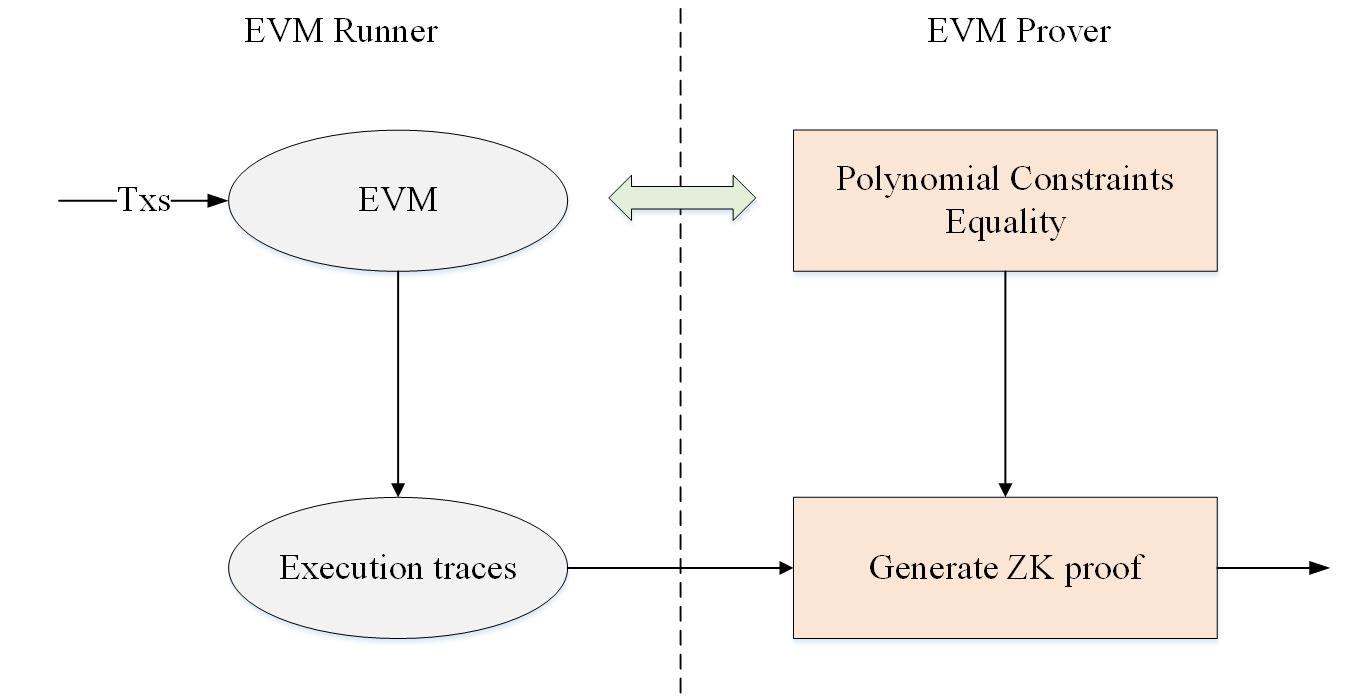
\includegraphics[width=0.8\textwidth]{zkevm-architecture-consensus-level.jpg}
    \caption{ZKEVM architecture based on Consensus-level}
    \label{fig:zkevm-architecture-consensus-level}
\end{figure}

The main workload of this scheme lies in the design of ZK constraints which does not require any modifications to EVM. Which is advantageous, but it is also disadvantageous because there are ZK-unfriendly operations in EVM that also must be proven by ZK-constraints, which makes the overall ZK efficiency low.

\subsubsection{Bytecode-level Compatibility}

Intuitively you may assume that the feature of this scheme is that it can process all the instructions of EVM on Bytecode-level (That the bytecodes of a Solidity contract can be directly used as input), however, other parts than the instructions can be different, such as getting a different state root and using a different hash algorithm. The framework of the scheme is shown in Figure \ref{fig:zkevm-architecture-bytecode-level}.
\begin{figure}[!ht]
    \centering
    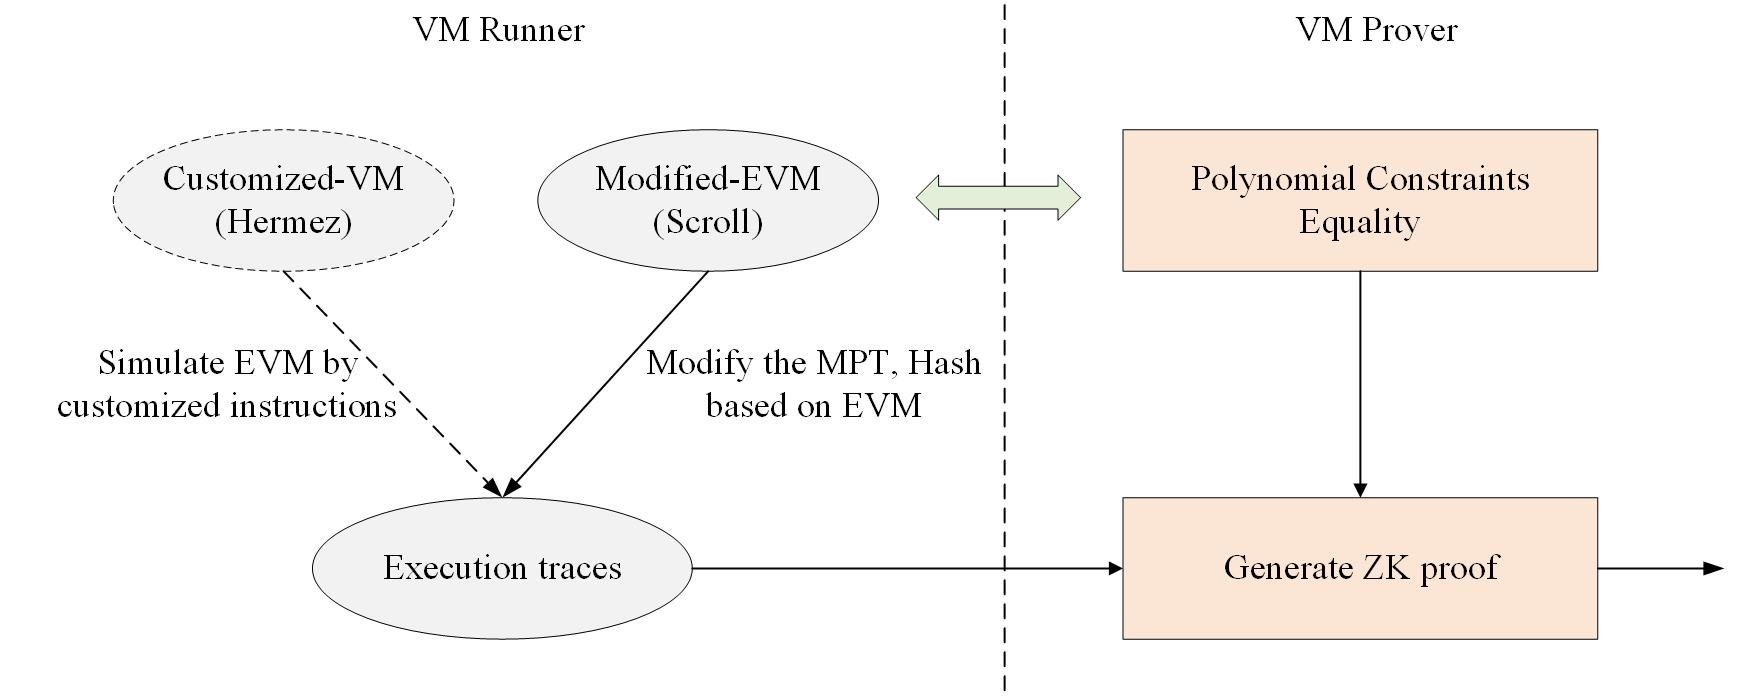
\includegraphics[width=0.8\textwidth]{zkevm-architecture-bytecode-level.jpg}
    \caption{ZKEVM architecture based on Bytecode-level}
    \label{fig:zkevm-architecture-bytecode-level}
\end{figure}

As you can tell by this scheme it requires designing or modifying the VM in addition to designing ZK constraints. As an example, Scroll may only need to make corresponding modifications based on the Ethereum client, but Hermez is slightly more complicated due to them customizing a VM. Compared with the Consensus-level ZKEVM scheme, the ZK efficiency of this scheme is slightly better.

\subsubsection{Language-level Compatibility}

Compared to previous two schemes, Language-level compatibility is the weakest. It does not have to be 100\% compatible with EVM, which means that simple modifications to some contracts could result in it needing a lot of support. However, the overall scheme has a ZK-friendly design, e.g, the memory model, instruction set, account model and so on, hence it has a better ZK efficiency. The framework of this scheme is shown in Figure \ref{fig:zkevm-architecture-language-level}.
\begin{figure}[!ht]
    \centering
    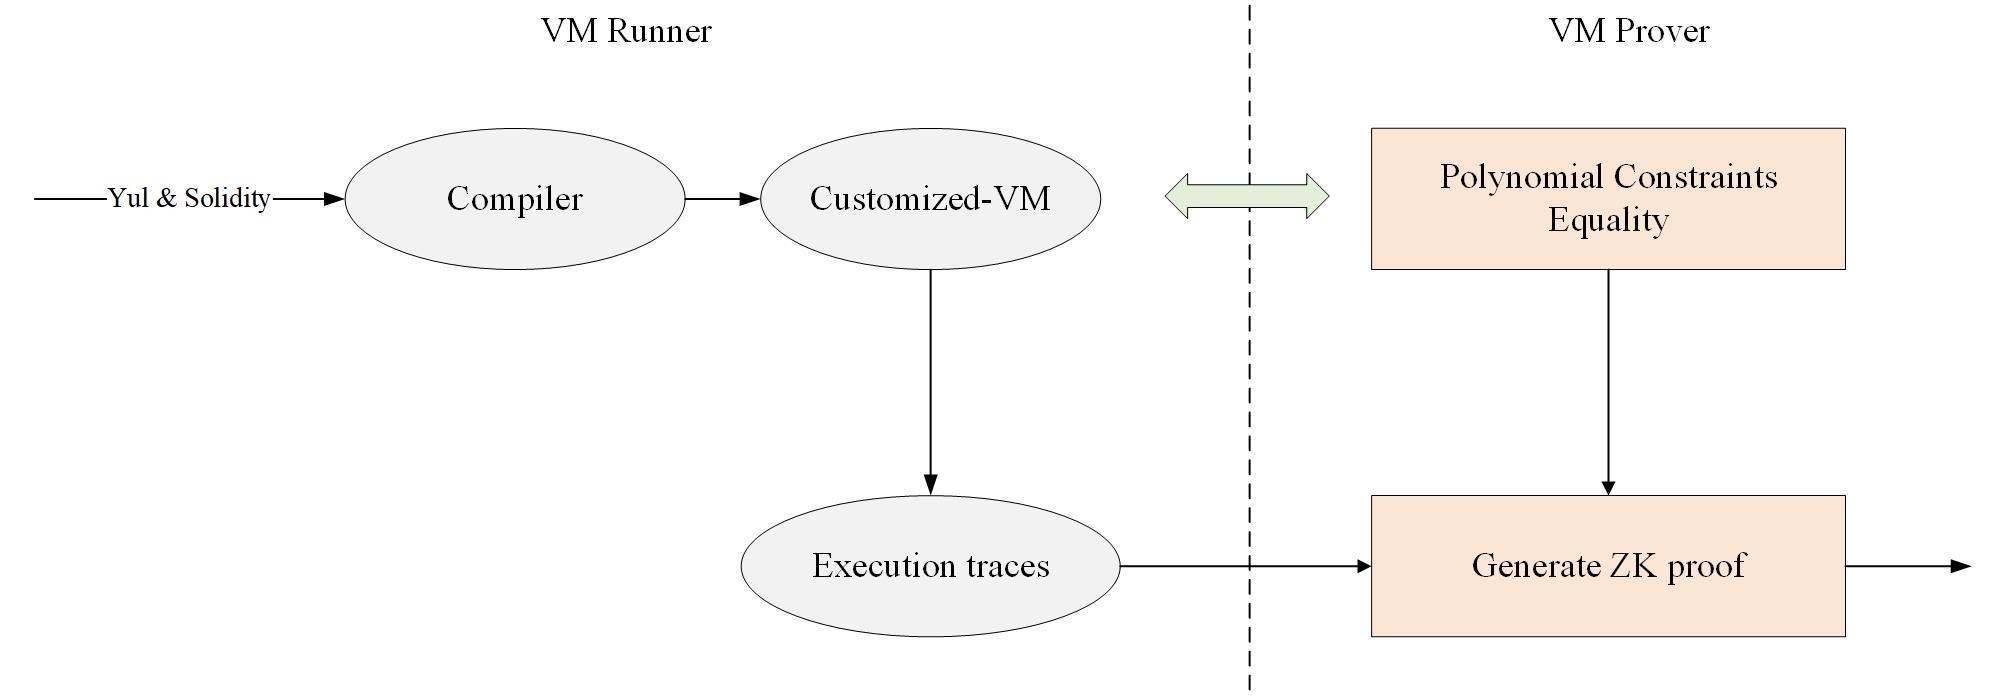
\includegraphics[width=0.8\textwidth]{zkevm-architecture-language-level.jpg}
    \caption{ZKEVM architecture based on Language-level}
    \label{fig:zkevm-architecture-language-level}
\end{figure}

Out of all the schemes this has the highest workload, involving the compiler, VM \& constraint design and so on. However, it is also achieving the best ZK efficiency. An example would be StarkWare's Cairo VM, which has a surprisingly good performance in terms of capacity expansion. StarkWare team has come quite far with the Cairo design in terms of being ZK-friendly since the inception of teams pursuing developing a ZKEVM solution.

\subsection{Our Work}

Designing and implementing a fully functional ZKEVM is a very daunting and challenging task. We have thoroughly studied and followed the progress of other teams in this space, and mastered how to design an efficient ZK-friendly EVM.

OlaVM is designed to have strong EVM compatibility without compromising its ZK-friendliness. To maintain its ZK-friendliness we've defined a simple instruction set, which makes the underlying state transition constraints very concise. In addition to this, OlaVM is a register-based VM, which significantly reduces the execution trace (avoiding intensive PUSH and POP operations compared to a stack-based VM). The Word of OlaVM is an element defined in a finite field, that's how we are able to obtain a simplified set of instructions. Finally, OlaVM supports some neat tricks to prevent the VM itself from performing complex calculations, reducing the execution trace and thereby improving overall ZK efficiency. We have defined integer calculation logic of uint256 to achieve solid EVM compatibility. In order to reduce the execution trace of integer calculation, we use BLS12-381 curve, which is defined on a 381-bit characteristic finite field.

In terms of design, based on the technical characteristics described above, OlaVM generates smaller execution traces and more concise state transition constraints, which enables us to achieve better ZK efficiency.

In addition to that we utilize other technical means such as reducing the number of selector polynomials by Combined Selector technology, as well as reducing the constraint scale using Lookup Argument technology, in order to improve ZK efficiency. For detailed principle, please refer to Section \ref{sec:key-technologies}. To further improve ZK efficiency, we have got a ZK hardware acceleration design framework. In order to ensure scalability of the design, we only accelerate the core module in ZK algorithm -- MSM (Multi-Scalar Multiplication), so that our design still applies to other ZK algorithms.

OlaVM uses a ZK algorithm without FFT in our design (for detailed principle, please refer to Section \ref{sec:zk-without-fft}), not simply a classic ZK algorithm, such as Halo2 \cite{website:halo2}, Plonk \cite{cryptoeprint:2019/953}, Plonky2 \cite{website:plonky2} and Groth16 \cite{Groth16}. Reasoning behind this is, with ZK algorithms, although FFT/IFFT and MSM calculations occupy most of the execution time of the entire algorithm, due to the computational complexity of FFT being $O(N\log N)$ and the MSM being $O(N/\log N)$ (Do note that at this complexity, a lot of hardware buffers are required), as the circuit size increases, FFT/IFFT will consume more computing resources than MSM (MSM has more multipliers than FFT/IFFT for a single multiplication even if for the bit width).

It should be noted that compared to the traditional ZK algorithms of R1CS system, such as BCTV14 \cite{ben2014succinct}, Halo \cite{cryptoeprint:2019/1021} and Fractal \cite{Fractal}, current ZK algorithms without FFT based on R1CS system, such as Nova \cite{cryptoeprint:2021/370} and Spartan \cite{Spartan}, has more efficient performance in proving, verifying, recursive performance and so on.

We believe that a ZK algorithm without FFT based on Plonkish constraint system will have better performance, although it is not considering optimal now, we will continue studying and researching this, as well as showcasing the hardware acceleration scheme of its main computing module, MSM, in advance.

\subsection{Outline of the Paper}

The remaining sections of this paper are summarized as follows:
\begin{itemize}
    \item Section \ref{sec:overview-of-vm} mainly describes the design of the virtual machine of OlaVM, which is the basis for OlaVM to obtain smaller execution traces and state transition constraints;
    \item Section \ref{sec:overview-of-zkvm-architecture} mainly describes the design of OlaVM constraints, covering the design idea of OlaVM architecture;
    \item Section \ref{sec:structure-of-execution-trace-table} mainly describes the data structure of execution traces and the structure description of related sub-traces;
    \item Section \ref{sec:circuit-constraint} mainly describes the underlying constraints of OlaVM, primarily constraints relating to the instruction set;
    \item Section \ref{sec:builtins} mainly describes the custom constraints supported in OlaVM, called Builtins;
    \item Section \ref{sec:storage-module} mainly describes the account model used in OlaVM and the corresponding constraint logic;
    \item Section \ref{sec:integer-arithmetic-operation} mainly describes uint256 integer calculation logic supported in OlaVM;
    \item Section \ref{sec:zk-without-fft} mainly describes the principle of ZK without FFT algorithm;
    \item Section \ref{sec:zk-acceleration} mainly describes MSM algorithm and the design framework of FPGA-accelerated MSM;
    \item Section \ref{sec:key-technologies} mainly describes the key technologies used in the entire design of OlaVM.
\end{itemize}


    \section{Overview of VM} \label{sec:overview-of-vm}

This section introduces the basic design ideas of OlaVM, primarily focusing on
(1) why we choose a register-based VM instead of a stack-based VM;
(2) how to design function calls on a register-based VM;
(3) defining VM instructions on a finite field for better proving efficiency;
(4) simplified VM instruction set design;
(5) structure description of the VM instructions.

\subsection{Register-based VM}

Among virtual machine architectures, stack-based and register-based are common implementations. Stack-based implementation is used by e.g, Java VM \cite{gunther2019scenery} and EVM \cite{website:evm}, and register-based virtual machine implementations by e.g, Lua VM \cite{ierusalimschy2005implementation} and Cairo VM \cite{cryptoeprint:2021/1063}. These two types of virtual machines adopt the mode of simulating physical CPU to execute instructions, but there are significant differences in execution efficiency and the speed of compiling and generating code in this specific implementation process. Take a simple addition instruction as an example to illustrate the difference between two virtual machine architectures in the process of executing instructions. The storage data structure of a stack-based virtual machine adopts the operation form of FIFO (First in, First out). First, the operand is popped out of the stack, and then the operation is performed, and the operation result will be pushed into the stack again. The instructions involved are
\begin{lstlisting}
POP (1)
POP (2)
ADD 1, 2, result
PUSH result
\end{lstlisting}
As can be seen in the addition operation, 4 instructions are required, which is relatively inefficient, however, the advantage is that you don't need to know the specific address of the operand, and you can get the operand by using instruction \verb|POP|.

Register-based VMs do not have such an operand stack to store operands. Each instruction will contain the register address of the operand. The above example involves the following instruction
\begin{lstlisting}
ADD R0, R1, R2
\end{lstlisting}

The obvious advantage of register-based virtual machines is that the addition can be completed with a single instruction. The disadvantage is that the address of the operand needs to be included in the instruction, which makes the instruction length longer.

Two virtual machine architectures each have their own advantages and disadvantages, further comparisons are shown in Table \ref{table:stacked-or-register}. Since our goal is to design a ZK-friendly virtual machine, we aim to achieve smaller execution traces of a given program with the trade-off increased instruction length. Furthermore, register-based virtual machines are easier to optimize during its execution of the instructions, hence, execution speed will see a significant improvement. Therefore we have opted for using a register-based virtual machine.
\begin{table}[!ht]
    \centering
    \begin{tabular}{|c|c|}
    \hline
        \emph{Stack-based VM vs. Register-based VM} & \emph{Comparison} \\ \hline
        Number of instructions & Register-based $<$ Stack-based \\
        Instruction length & Register-based $>$ Stack-based \\
        Difficulty of the code generation & Register-based $>$ Stack-based \\
        Instruction optimization & Register-based VM is easier to optimize code \\
        Execution speed & Register-based VMs have a faster execution pace \\ \hline
    \end{tabular}
    \caption{Stack-based VMs vs. Register-based VMs}
    \label{table:stacked-or-register}
\end{table}

\subsection{Function Call by RPR}

OlaVM adopts the register-based model. In order to easier simulate the effect of a function call stack it is necessary to save the next \verb|pc| that currently calls the initiating function to a dedicated read-only memory, RPR (Return PC ROM), which is convenient to find the \verb|pc| position that the last call should return to after the execution of the sub-function. The function call involves two instructions, \verb|CALL| and \verb|RET|, and a special register \verb|fp|, which points to the address of RPR. Figure \ref{fig:function-call-example} shows a function call example.
\begin{figure}[!ht]
    \centering
    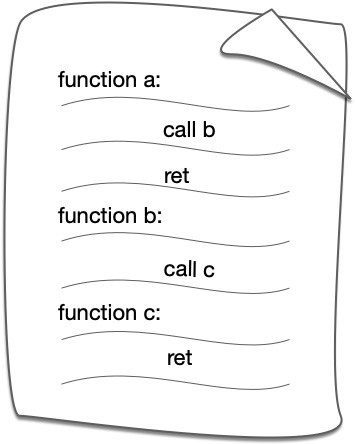
\includegraphics[width=0.3\textwidth]{function-call-example.jpg}
    \caption{Function call example}
    \label{fig:function-call-example}
\end{figure}

The stack frame of the above function call is shown in Figure \ref{fig:function-call-frame}.
\begin{figure}[!ht]
    \centering
    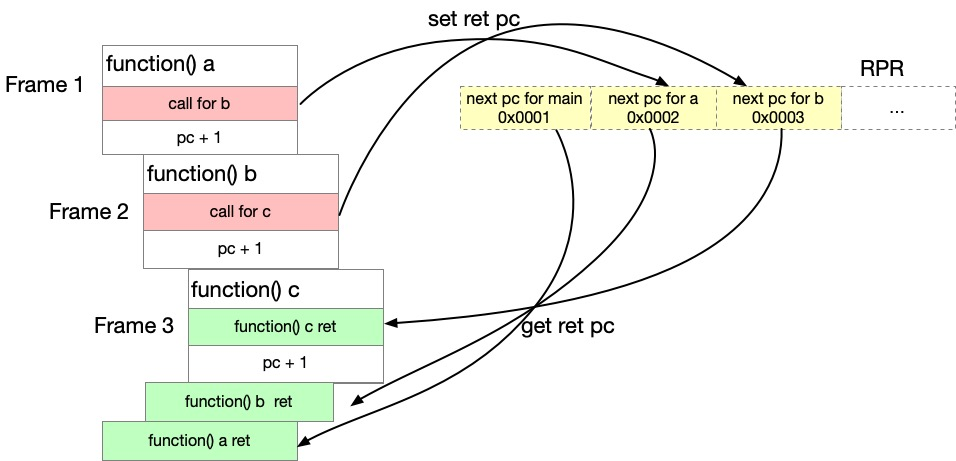
\includegraphics[width=0.8\textwidth]{function-call-frame.jpg}
    \caption{Function call frame}
    \label{fig:function-call-frame}
\end{figure}

\begin{itemize}
    \item RPR stores 3 return \verb|pc| positions: \verb|a return -> main pc|, \verb|b return -> a pc|, \verb|c return -> b pc|;
    \item When function \verb|main| utilizes instruction \verb|CALL| to call function \verb|a|, the value of \verb|pc| will be updated to the value saved in register \verb|r0|;
    \item Set the value of ROM location pointed by the pointer stored in register \verb|fp| to current \verb|pc+1|, \verb|fp+1| points to the next empty memory area.
    \item When the function a completes the execution, it will take the value pointing to the correct position of ROM through the pointer stored in register \verb|fp|. Set current \verb|pc| to this value, so the remaining program fragments can be executed when returning to function main;
    \item \verb|fp| points to the position of \verb|fp-1| in RPR;
    \item For nested calls of function \verb|b| and function \verb|c|, the change process of \verb|pc| and \verb|fp| is the same as above.
\end{itemize}

\subsection{Word in Finite Field}

In order to make the processing logic of the VM simple, to obtain the smallest basic constraint unit (which can constrain any instruction of the VM), we defined the VM over a finite field so that the Word of the VM is a field element. Therefore, the calculation logic of the VM only supports a few simple field operations, such as addition, subtraction (equivalent to adding an additive inverse), multiplication, and division (equivalent to multiplying a multiplicative inverse). Meanwhile, we have also implemented integer calculation logic in order to support integer operations (OlaVM supports uint256 integer calculations to strengthen compatibility with Ethereum). The relationship between integer calculation and field calculation is shown in Figure \ref{fig:field-operation}.
\begin{figure}[!ht]
    \centering
    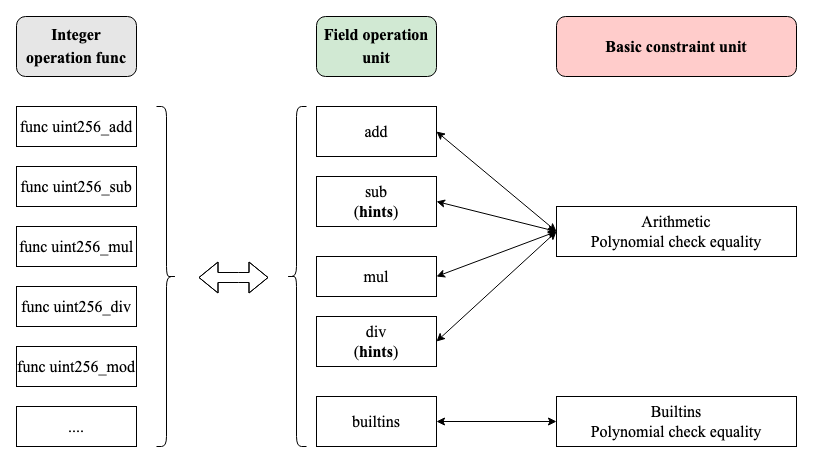
\includegraphics[width=0.6\textwidth]{field-operation.png}
    \caption{Field operation}
    \label{fig:field-operation}
\end{figure}

As you can tell, OlaVM instruction set defined over a finite field are very concise, with only a few instructions, hence the number of constraint units of the circuit will be very small. In PSE scheme, the underlying constraint unit needs to process the logic of all EVM instructions, which adds up to roughly 100 instructions, vastly increasing its complexity. In addition to this, we have defined some builtins in order to support more complex logic. Thanks to this, given complex calculations that needs to be implemented, we don't need to utilize these VM instructions, we can pre-implement the corresponding custom constraint logic and call that directly.

\emph{Note:} Current choice of finite field is BLS12-381 curve, which is planned to support uint256 integer calculations (refer to the design of StarkWare \cite{website:starkware}).

\subsection{Instruction Set} \label{subsec:instruction-set}

Whilst designing a ZKVM we also considered the complexity of verification, in addition to the execution efficiency of the VM itself, which differs from the traditional design principles of the instruction set. Purely pursuing efficient execution of instructions is not our goal, we have other fundamental design objectives, such as achieving short and concise verification complexity (occupying fewer trace cell units).

For example: when you have two instruction sets $A$ and $B$, there is an ``is\_zero" instruction in instruction set $A$, which is used to judge ``if x = 0, res = 1, otherwise, res = 0”, and except for this instruction, instruction set $B$ is identical to instruction set $A$. We denote the number of track units occupied by a CPU based on instruction set $A$ to execute an instruction by $a$ (for simplicity, assuming that all instructions consume the same number of units), and the number of track units required to execute one step based on instruction set $B$ by $b$ (where $a>b$ due to the added complexity of additional instructions). On the other hand, if a deterministic program is written based on instruction set $A$, it will execute $k_A$; and if it's written based on instruction set $B$, it will execute $k_B$ ($k_B>k_A$, it is possible to utilize more instructions to execute ``is\_zero”). If $a \cdot k_A < b \cdot k_B$, instruction set $A$ is more suitable for this program; conversely, instruction set $B$ is more suitable. When deciding whether to intervene in an instruction, we should consider the relationship between the additional cost of each step ($a/b$) and the additional steps added ($k_A/k_B$).

Based on the principles above, the instruction sets we designed are as shown in Table \ref{table:instruction-set}, \verb|flag| is a special register that stores the flag of \verb|overflow| or \verb|borrow|.
\begin{table}[!ht]
    \resizebox{\textwidth}{!}{
    \begin{tabular}{|c|c|c|c|l|c|}
    \hline
    \emph{Type} & \emph{Sub Type} & \emph{Instruction} & \emph{Operands} & \emph{Description} & \emph{flag} \\ \hline
    \multirow{4}{*}{Logic} & \multirow{4}{*}{arithmetic} & ADD & r0 r1 r2 & Compute [r1] + [r2] and store the result in r0 & overflow \\ \cline{3-6}
    & & SUB & r0 r1 r2 & Compute [r1] - [r2] and store the result in r0 & borrow \\ \cline{3-6}
    & & MUL & r0 r1 r2 & Compute [r1] * [r2] and store the least significant bits of the result in r0 & overflow \\ \cline{3-6}
    & & DIV & r0 r1 r2 & Compute [r1] / [r2] and store the result in r0 & [r2] = 0 \\ \hline
    \multirow{7}{*}{Flow} & \multirow{2}{*}{jump} & JMP & r0 & Set pc to [r0] & \\ \cline{3-6}
    & & CJMP & r0 & If flag = 1, set pc to [r0], else increment pc as usual & \\ \cline{2-6}
    & \multirow{3}{*}{call} & \multirow{3}{*}{CALL} & \multirow{3}{*}{r0} & Call instruction is usually used to make a call from one function to another & \multirow{3}{*}{} \\
    & & & & Set pc to [r0], and store next pc in RPR & \\
    & & & & Update the value saved in RPR position pointed to by fp to next pc, then fp = fp + 1 & \\ \cline{2-6}
    & ret & RET & & Update the value saved by pc to the next pc value of RPR pointed to by fp, then fp = fp - 1 & \\ \cline{2-6}
    & end & END & & END means the program is terminated and all registers are cleared & \\ \hline
    \multirow{2}{*}{Move} & \multirow{2}{*}{mov} & MOV & r0 r1 & Store [r1] in r0 & \\ \cline{3-6}
    & & MOVI & r0 imm0 & Store immediate value imm0 in r0 & \\ \hline
    \multirow{6}{*}{RAM} & \multirow{2}{*}{memory} & MLOAD & r0 r1 & Load the Word in memory begin with offset [r1] and store the Word into r0 & \\ \cline{3-6}
    & & MSTORE & r1 r0 & Store [r0] at the start of memory where the offset is [r1] & \\ \cline{2-6}
    & \multirow{4}{*}{storage} & \multirow{2}{*}{SLOAD} & \multirow{2}{*}{r0 r1} & Use [r1] as key, query the value of the key from storage & \\
    & & & & (the key will be hashed and prefixed with a splice) and store it in r0 & \\ \cline{3-6}
    & & \multirow{2}{*}{SSTORE} & \multirow{2}{*}{r1 r0} & Use [r1] as key, [r0] as value, store the key and the value into storage & \\
    & & & & (the key will be hashed and prefixed with a splice) & \\ \hline
    Input & input & READ & r0 & Read the external input from VM freeInput, and store one Word into r0 & \\ \hline
    \end{tabular}
    }
    \caption{Instruction set}
    \label{table:instruction-set}
\end{table}

\emph{Note:} We haven't designed comparison instructions because comparison operations can be implemented directly through multiple Range Checks based on the particular design and parameter selection of OlaVM. Specific principles of this will be introduced in later sections.

\subsection{Instruction Structure} \label{subsec:instruction-structure}

Based on the VM instruction set defined in Section \ref{subsec:instruction-set}, the VM is able to execute programs. OlaVM proof system can constrain the semantics of each instruction according to the execution trace of the VM to ensure that the program has been executed correctly. However, we also need to ensure that the actual program being executed has not been maliciously modified, meaning, we have to ensure it executed the original, correct program. As for how to check that the instructions involved in the execution trace are all present in the original program fragment and if they are executed in the correct \verb|pc| order, we've decided to compare whether or not each instruction in the execution trace is included in the original program. In order to do that, we encode each instruction, then checking if the encoding of the execution instruction is included in the encoding of the program instruction.

Instruction encoding form as shown in Figure \ref{fig:instruction-encoding} with each instruction encoding occupying 32 bits.
\begin{figure}[!ht]
    \centering
    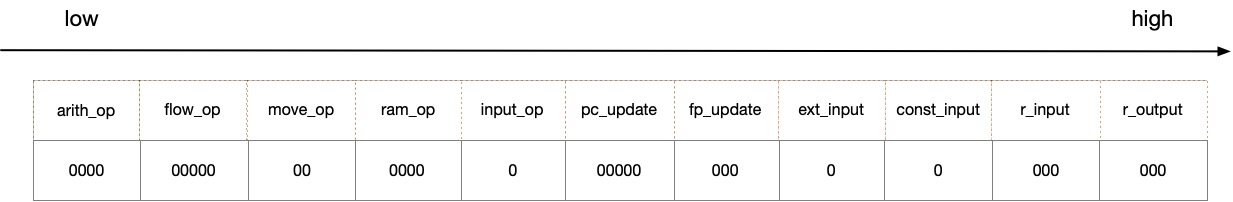
\includegraphics[width=\textwidth]{instruction-encode.jpg}
    \caption{Instruction encoding}
    \label{fig:instruction-encoding}
\end{figure}

As shown in Table \ref{fig:instruction-encoding}, the instruction will set the bit value of each used item to 1 and set the unused item to 0 when encoding. The specific meaning of each item is explained as follows:
\begin{itemize}
    \item \verb|arith_op| is the logic of arithmetic operation, which occupies 4 bits and is used to select the 4 instructions of \verb|ADD|, \verb|SUB|, \verb|MUL| and \verb|DIV|;
    \item \verb|flow_op| is the control logic, which occupies 5 bits and is used to indicate the selection of control-related instructions;
    \item \verb|mov_op| is the register move logic, which occupies 2 bits and is used to indicate the selection of \verb|mov|-related instructions;
    \item \verb|ram_op| is the operation logic of memory and storage, which occupies 4 bits and is used to indicate the selection of specific operations;
    \item \verb|input_op| is the input logic, which occupies 1 bit and is used to indicate the selection of the program to read the input from outside;
    \item \verb|pc_update|, occupying 5 bits, is used to indicate the relevant logic of \verb|pc| update. \verb|pc| can be updated through \verb|flow_op| or updated normally, and the \verb|pc_update| value of normal update is 00000;
    \item \verb|fp_update|, occupying 3 bits, is used to indicate whether \verb|fp| is updated. Instructions \verb|CALL|, \verb|RET| and \verb|END| will update \verb|fp|;
    \item \verb|ext_input|, occupying 1 bit, is used to indicate whether there is an external input;
    \item \verb|const_input|, occupying 1 bit, is used to indicate whether the instruction has immediate value input;
    \item \verb|r_input|, occupying 3 bits, is used to indicate whether the instruction read input values from three registers \verb|r0|, \verb|r1| and \verb|r2|;
    \item \verb|r_output|, occupying 3 bits, is used to indicate whether the instruction will update the value of three registers \verb|r0|, \verb|r1| and \verb|r2|.
\end{itemize}

\noindent
The encoding forms of \verb|arith_op| are
\begin{lstlisting}
0001 -> ADD
0010 -> SUB
0100 -> MUL
1000 -> DIV
\end{lstlisting}
The encoding forms of \verb|flow_op| are
\begin{lstlisting}
00001 -> JMP
00010 -> CJMP
00100 -> CALL
01000 -> RET
10000 -> END
\end{lstlisting}
The encoding forms of \verb|mov_op| are
\begin{lstlisting}
01 -> MOV
10 -> MOVI
\end{lstlisting}
The encoding forms of \verb|ram_op| are
\begin{lstlisting}
0001 -> MSTORE
0010 -> MLOAD
0100 -> SSTORE
1000 -> SLOAD
\end{lstlisting}
The encoding form of \verb|input_op| is
\begin{lstlisting}
1 -> READ
\end{lstlisting}
The encoding forms of \verb|pc_update| are
\begin{lstlisting}
00001 indicates pc changes caused by JMP
00010 indicates pc changes caused by CJMP
00100 indicates pc changes caused by CALL
01000 indicates pc changes caused by RET
10000 indicates pc changes caused by END
\end{lstlisting}
The encoding forms of \verb|pc_update| are
\begin{lstlisting}
01 indicates the change of the fp register pointer caused by the CALL instruction
10 indicates the change of the fp register pointer caused by the RET instruction
\end{lstlisting}
The encoding forms of \verb|fp_update| are
\begin{lstlisting}
001 indicates the content change of the fp register caused by the CALL instruction
010 indicates the content change of the fp register caused by the RET instruction
100 indicates the content change of the fp register caused by the END instruction
\end{lstlisting}
The encoding forms of \verb|ext_input| are
\begin{lstlisting}
1 indicates the existence of external input data
\end{lstlisting}
The encoding form of \verb|const_input| is
\begin{lstlisting}
1 indicates that mov instruction has immediate value input
\end{lstlisting}
The encoding form of \verb|r_input| is as follows
\begin{lstlisting}
001/010/100 indicates the input of register r0, r1 and r2 respectively
\end{lstlisting}
The encoding form of \verb|r_output| is as follows
\begin{lstlisting}
001/010/100 indicates the output of register r0, r1 and r2 respectively
\end{lstlisting}

The description above contains instruction encoding forms, without immediate value encoding forms of the instruction. If an instruction involves immediate value, we will encode the immediate value after the instruction. At this time, \verb|pc| is increased by the size of instruction each time, namely \verb|pc = pc + instruction_size|.

With the above code rules, we can prove that the executed program fragment is indeed derived from the original program. In order to ensure the execution of the correct program sequence in case of program jumps, an additional \verb|pc| code to the instruction is required to prove the program is executed in the correct sequence.


    \section{Overview of ZKVM Architecture} \label{sec:overview-of-zkvm-architecture}

Our architectural approach is modular, designing the ZKVM to divide traces into main and sub traces. This section will describe the constraint list and consistency between main/sub traces, as well as between sub traces.

\subsection{Modular Design}

The modular design of OlaVM greatly improves the efficiency of the prover. Before we dive into a detailed description, let us briefly analyze the time consumption distribution chart of the VM executing a transaction, as show in Figure \ref{fig:vm-execution-proportion}.

\begin{figure}[!ht]
    \centering
    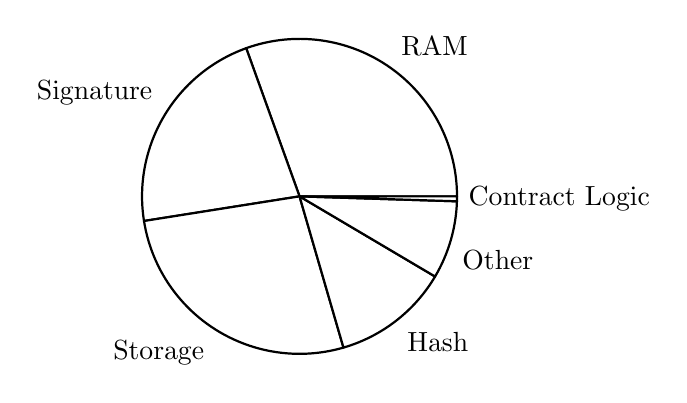
\begin{tikzpicture}
        \pie[radius=2, color=white, hide number]{
            30.5/RAM,
            22/Signature,
            27/Storage,
            12/Hash,
            8/Other,
            0.5/Contract Logic
        }
    \end{tikzpicture}
    \caption{VM Execution proportions} \label{fig:vm-execution-proportion}
\end{figure}

As can be seen from Figure \ref{fig:vm-execution-proportion}, the entire transaction execution process can be roughly divided into following categories: Contract Logic, RAM, Signature Verification, Storage Read/Write, Hash, and so on. If we prove these calculation types in a circuit, the entire constraint design will become quite complicated and difficult to handle, so we need to ``divide and conquer'' and finally processing them together, which is the source of the modular idea.

The execution trace of the VM (hereinafter referred to as the main trace for convenience) can be seen in Figure 9. With the approach mentioned above we divide the main trace table, resulting in several smaller tables, referred to as sub trace tables. Each sub trace table corresponds to a specific type of operation. Example given, the RAM sub trace table only contains RAM operations, and the signature sub trace table only contains signature operations. Therefore, we only need to design the corresponding constraint system for each module. The overall design framework is shown in Figure \ref{fig:zkvm-architecture}.

\begin{figure}[!ht]
    \centering
    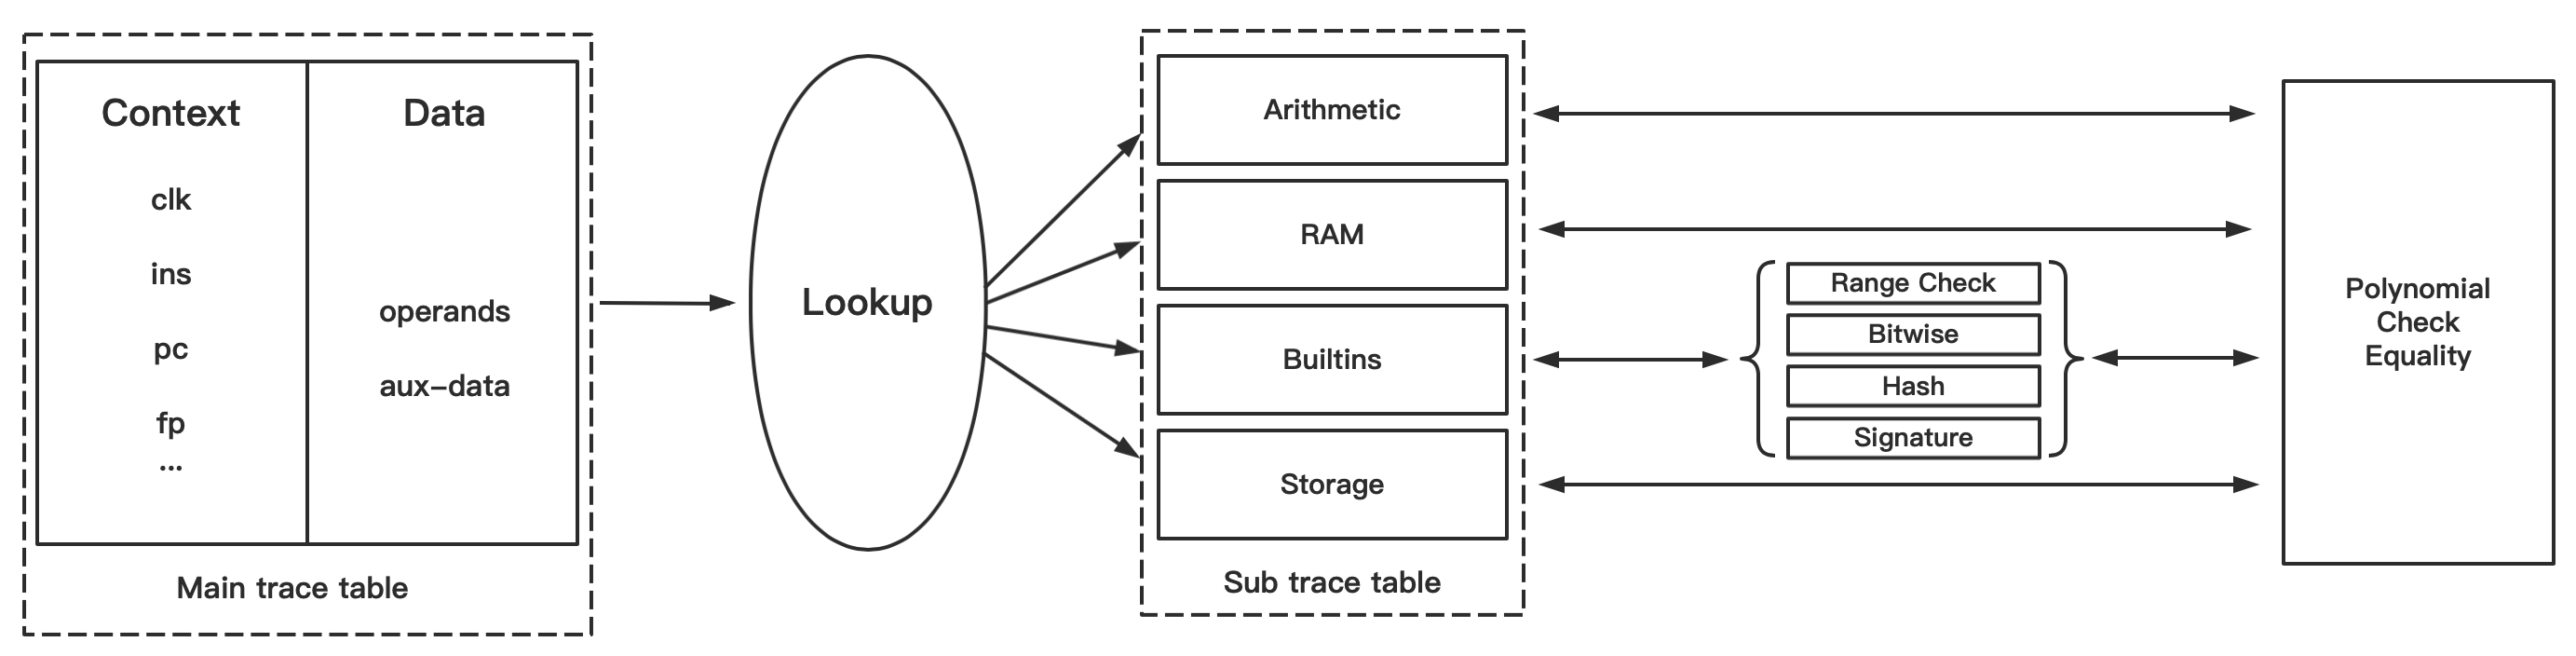
\includegraphics[width=\textwidth]{zkvm-architecture.png}
    \caption{Architecture of ZKVM}
    \label{fig:zkvm-architecture}
\end{figure}

The modular design approach allows for proofs among different modules to be executed in parallel, because the verification process is independent of each other, and the data correlation is only guaranteed by Permutation Argument and Lookup Argument, there are no data dependencies between each other. This is way more efficient than executing all the proofs in a single circuit, furthermore, multiple proofs corresponding to different sub-modules can be aggregated into a single proof, the idea of using recursive proofs can utilized to improve the system efficiency of proofs between different blocks.

These common technologies are all applied in OlaVM architecture.

\subsection{Consistency Check}

We need to check the consistency between main/sub traces to ensure that the trace data is consistent.

\subsubsection{Consistency between Main Trace and Sub Traces}

According to the definition of main/sub trace tables, elements of sub trace tables should be taken from the main trace table. For example, the RAM sub trace table is composed of all RAM operations in main trace table, the signature sub trace table is composed of all signature verification operations in the main trace table. Now we need to make sure that these are executed correctly. Lookup Argument gracefully achieves this through successfully binding the data relationship between the main trace table and the corresponding sub trace tables.

\begin{figure}[!ht]
    \centering
    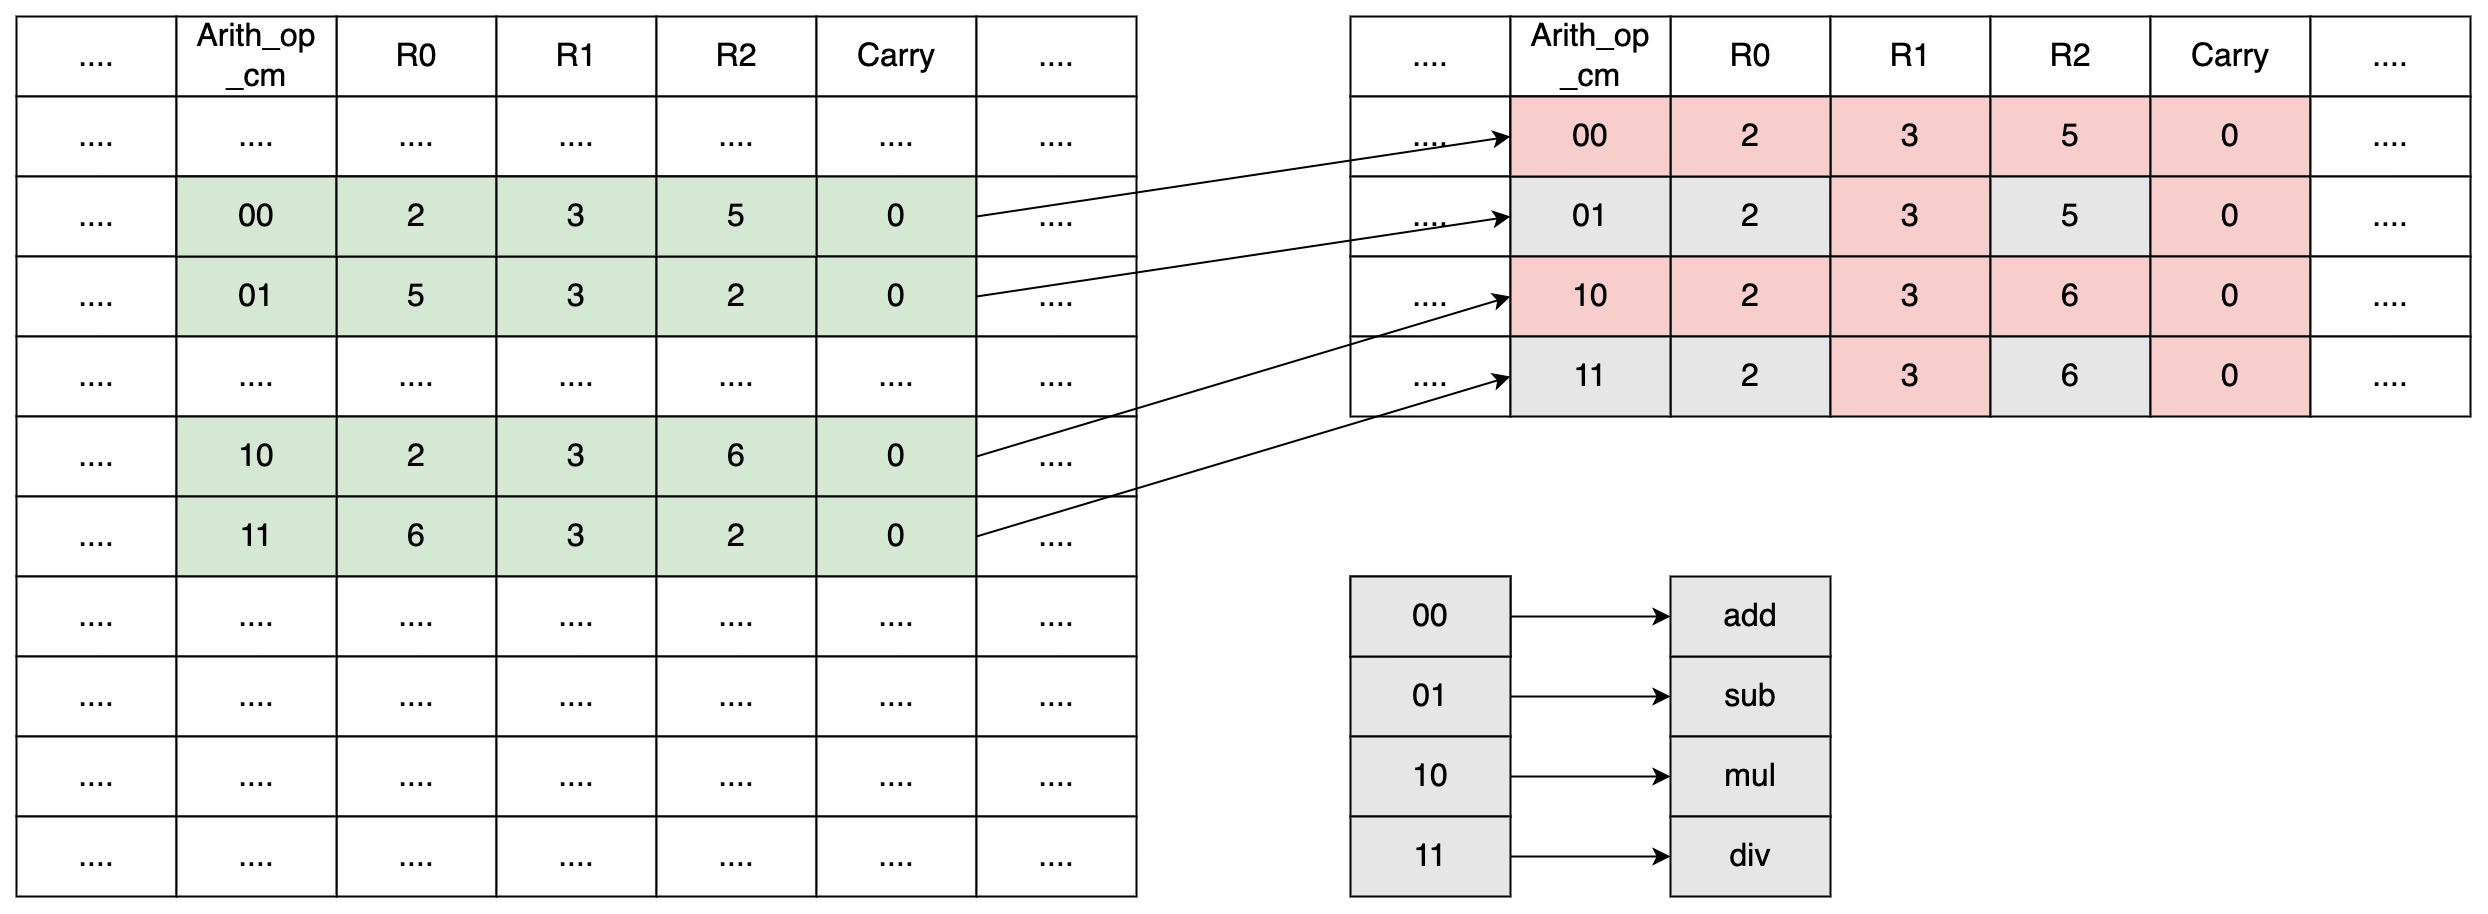
\includegraphics[width=0.8\textwidth]{main-sub-trace-lookup.jpg}
    \caption{Lookup between main trace and sub trace tables}
    \label{fig:main-sub-trace-lookup}
\end{figure}

\emph{Note:} We have adjusted subtraction and division for convenience (The gray marked part on the right side of Figure \ref{fig:main-sub-trace-lookup}), so that addition and subtraction can share one set of constraints and multiplication and division can share another set of constraints, which minimizes the overall constraints scale.

We utilize Lookup technology to ensure data consistency between the main trace table on the left and sub trace tables on the right, such as
\[ \{\text{arith\_op\_cm}, \text{R0}, \text{R1}, \text{R2}, \text{Carry}\}_\text{sub trace table} \subset \{\text{arith\_op\_cm}, \text{R0}, \text{R1}, \text{R2}, \text{Carry}\}_\text{main trace table} \]

Utilizing the following constraints to verify the validity of the data in sub trace tables
\begin{align*}
    f_{\text{arith\_op\_cm}}(x) \prod \left(3 - f_{\text{arith\_op\_cm}}(x)\right) \left(4 - f_{\text{arith\_op\_cm}}(x)\right) \left(f_{\text{R0}}(x) + f_{\text{R1}}(x) - (f_{\text{R2}}(x) + \mathrm{Bound} \cdot f_{\text{Carry}}(x))\right) &= 0, \\
    f_{\text{arith\_op\_cm}}(x) \prod \left(1 - f_{\text{arith\_op\_cm}}(x)\right) \left(2 - f_{\text{arith\_op\_cm}}(x)\right) \left(f_{\text{R0}}(x) \cdot f_{\text{R1}}(x) - (f_{\text{R2}}(x) + \mathrm{Bound} \cdot f_{\text{Carry}}(x))\right) &= 0.
\end{align*}

\emph{Note:} The idea of Combined Selector is adopted here to reduce the number of selector polynomials. Please refer to Section \ref{sec:key-technologies} for detailed principles.

\subsubsection{Consistency between Sub Traces}

As mentioned in the previous section, we ensure data consistency between the main/sub trace tables through Lookup Arguments, however, data consistency must also be maintained between sub trace tables. For example, we store the result of instruction \verb|ADD| in a result register, we must be able to ensure that the value written in this register is indeed the result of the execution of that previous instruction. Then we utilize Permutation Arguments to ensure data consistency between the arithmetic sub trace table and the RAM sub trace table.

During the execution of the entire VM, some of the operands of the instructions derive from intermediate values of the VM execution, when utilizing Permutation Argument to ensure data consistency as mentioned above, some derive from public inputs, such as the initial value and result of the program, we use instruction \verb|EQ| to ensure that the instruction does operate the correct value.
\begin{figure}[!ht]
    \centering
    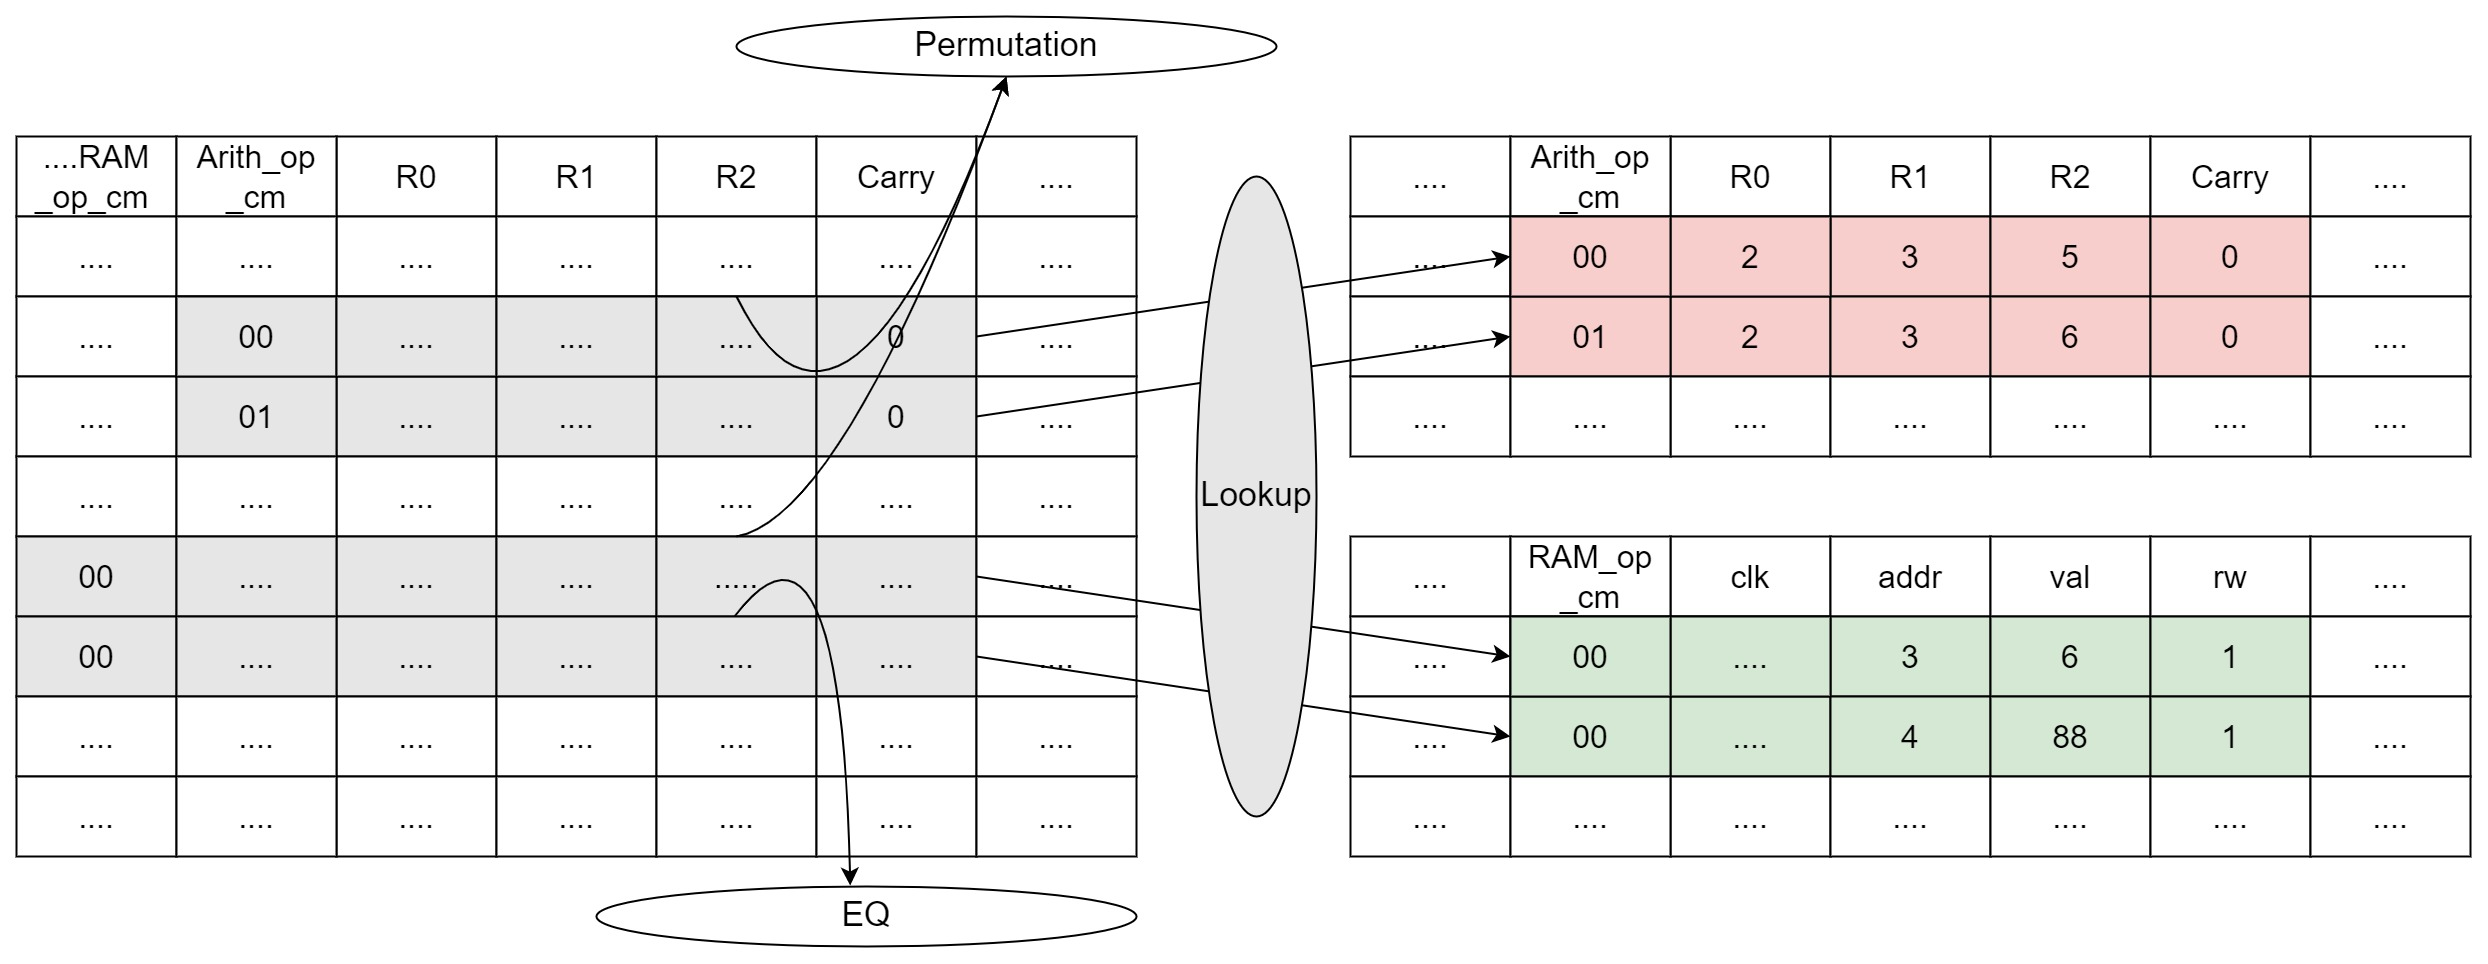
\includegraphics[width=\textwidth]{sub-sub-trace-lookup.jpg}
    \caption{Consistency between sub trace tables}
    \label{fig:sub-sub-trace-lookup}
\end{figure}

\subsection{Constraint List}

Because of the modular design, each module handles a specific function, resulting in specific constraints for each module, described in detail in later sections. Furthermore, we added context constraints, primarily used to constrain the change of context after the VM executes each instruction, this constraint applies to all instructions, hence applied to the main trace table.

According to the instruction structure we defined, it occupies 31 valid bits, enabling us to state the following definitions:

Arithmetic operations:
\begin{align*}
    f_\text{ADD} = f_{0},\ f_\text{SUB} = f_{1},\ f_\text{MUL} = f_{2},\ f_\text{DIV} = f_{3},
\end{align*}

Control flows:
\begin{align*}
    f_\text{JMP} = f_{4},\ f_\text{CJMP} = f_{5},\ f_\text{CALL} = f_{6},\ f_\text{RET} = f_{7},\ f_\text{END} = f_{8},
\end{align*}

Moves:
\begin{align*}
    f_\text{MOV} = f_{9},\ f_\text{MOVI} = f_{10},
\end{align*}

Memory and storage operations:
\begin{align*}
    f_\text{MLOAD} = f_{11},\ f_\text{MSTORE} = f_{12},\ f_\text{SLOAD} = f_{13},\ f_\text{SSTORE} = f_{14},
\end{align*}

External inputs:
\begin{align*}
    f_\text{INPUT} = f_{15},\ f_\text{EX\_INPUT} = f_{23},
\end{align*}

\verb|pc|:
\begin{align*}
    f_\text{PC\_CALL} = f_{16},\ f_\text{PC\_RET} = f_{17},\ f_\text{PC\_JMP} = f_{18},\ f_\text{PC\_CJMP} = f_{19},\ f_\text{PC\_END} = f_{20},
\end{align*}

\verb|fp| and \verb|const|:
\begin{align*}
    f_\text{FP\_CALL} = f_{21},\ f_\text{FP\_RET} = f_{22},\ f_\text{CONST} = f_{24}
\end{align*}

Inputs:
\begin{align*}
    f_\text{INPUT\_R0} = f_{25},\ f_\text{INPUT\_R1} = f_{26},\ f_\text{INPUT\_R2} = f_{27},
\end{align*}

Outputs:
\begin{align*}
    f_\text{UPDATE\_R0} = f_{28},\ f_\text{UPDATE\_R1} = f_{29},\ f_\text{UPDATE\_R2} = f_{30}.
\end{align*}

\subsubsection{Inst-decode Check}

Upon execution, the VM decodes the instruction, then performs the corresponding operation according to the parsed flag. Therefore, we need to verify that the instruction executed by the VM is valid, i.e.\ the value of the instruction encoding is consistent with the corresponding flag. For simplicity, we will not allocate a separate column (the length is $N$) for all flags, however, we will use a virtual column to represent (the length is $32N$). Therefore we define $\widetilde f_i = \sum_{j=i}^{30} 2^{j-i} f_j$, so $\widetilde f_0 = \sum_{j=0}^{30} 2^{j-0} f_j$, which represents the value of the first 31 bits of the instruction and $\widetilde f_{31} = 0$. In order to obtain the value of $f_i$ from $\{\widetilde f_i \}_{i=0}^{31}$, we utilize the equation
\begin{align*}
    \widetilde f_i - 2\widetilde f_{i+1} &= \sum_{j=i}^{30} 2^{j-i} f_j - 2 \sum_{j=i+1}^{30} 2^{j-i-1} f_j \\
    &= \sum_{j=i}^{30} 2^{j-i} f_j - \sum_{j=i+1}^{30} 2^{j-i} f_j. \\
    &= f_i
\end{align*}

The corresponding constraints are as follows:

Instruction:
\[ \text{instruction} = \widetilde f_0, \]

Bit:
\[ (\widetilde f_i - 2\widetilde f_{i+1} )(\widetilde f_i - 2\widetilde f_{i+1} - 1) = 0, \qquad \forall i \in [0,31), \]

Last value is zero:
\[ \widetilde f_{31} = 0. \]

\subsubsection{Context Update}

If the instruction is \verb|JMP| or \verb|CJMP|, \verb|pc| is updated to the specified location \verb|dst_pc|, and register \verb|fp| stores the address of RPR.

If the instruction is \verb|CALL|, \verb|pc| is updated to the value in \verb|r0|, and the value of the location where \verb|fp| points to the RPR is set to \verb|pc+instruction_size|. \verb|fp+1| points to an empty memory area.

If the instruction is \verb|RET|, the function call ends, and \verb|pc| is updated to the value saved by the RPR pointed to by \verb|fp|, and \verb|fp| is updated to the value of \verb|fp-1| in RPR.

\begin{multline*}
    f_\text{pc}(x\omega) - f_\text{PC\_*JMP}(f_\text{dst\_{pc}}(x) + f_\text{PC\_CALL}(f_\text{dst\_{pc}}(x)) +f_\text{PC\_RET}(f_\text{fp}(x)) + \\
    (1 - f_\text{PC\_*JMP} - f_\text{PC\_CALL} - f_\text{PC\_RET})(f_\text{pc}(x) + \text{instruction\_size})) = 0,
\end{multline*}

\[ f_\text{FP\_CALL}(f_\text{fp}(x\omega) - (f_\text{pc}(x) + \text{instruction\_size})) = 0. \]

\subsubsection{Register Check}

We have three general-purpose registers. Most of the instructions are based on registers. During execution of instructions, some register states may change while others stay the same, based on which the instruction is being executed. We define flags to indicate the register read/write state corresponding to the current instruction. We can constrain these general-purpose registers through flags:
\begin{align*}
    (1 - f_\text{r0\_output})(f_\text{r0}(x\omega) - f_\text{r0}(x)) &= 0, \\
    (1 - f_\text{r1\_output})(f_\text{r1}(x\omega) - f_\text{r1}(x)) &= 0, \\
    (1 - f_\text{r2\_output})(f_\text{r2}(x\omega) - f_\text{r2}(x)) &= 0.
\end{align*}

The above constraints ensures that if the current instruction did not update the corresponding register, the value inside the register should stay the same, if the value of a certain register changed, we will ensure the validity of the value change on the corresponding sub trace table. For example, when executing the instruction \verb|ADD r0,r1,r2|, we will verify that the value inside register \verb|r1| and register \verb|r2| remains the same, then check \verb|r0=r1+r2| on the arithmetic sub trace table.

\subsubsection{Execute Correct Program}

The constraints described in previous sections guarantee the correctness of all the instructions executed by the VM, but there is no guarantee that the programs corresponding to these instructions are correct, i.e.\ corresponding to our original program. Therefore, we also need to verify that we have executed the correct program. Example given, we have the following program and store it in ROM:

\begin{table}[!ht]
    \centering
    \begin{tabular}{|c|c|c|}
    \hline
        \emph{pc} & \emph{Program Bytecodes} & \emph{program\_encode} \\ \hline
        0 & READ R0 & 0000000000000001000000001000010000 \\
        1 & MOV R1 3 & 0000000001000000000000000100001001 \\
        2 & ADD R0, R1, R2 & 0001000000000000000000000011000110 \\
        3 & END & 0000100000000000100000000000011111 \\ \hline
    \end{tabular}
    \caption{Simple VM example}
    \label{table:simple-vm-example}
\end{table}

Given an input, we get the execution trace table as shown in Table \ref{table:execution-trace-encoding}.

\begin{table}[!ht]
    \resizebox{\textwidth}{!}{
    \begin{tabular}{|c|c|c|c|c|c|c|c|c|c|c|c|c|c|}
    \hline
    clk & program\_encode & arith\_op & flow\_op & move\_op & ram\_op & input\_op & pc\_update & fp\_update & ext\_input & const\_input & r\_input & r\_output & pc \\ \hline
    0 & 0000000000000001000000001000010000 & 0000 & 00000 & 00 & 0000 & 1 & 00000 & 000 & 1 & 0 & 000 & 100 & 0 \\
    1 & 0000000001000000000000000100001001 & 0000 & 00000 & 10 & 0000 & 0 & 00000 & 000 & 0 & 1 & 000 & 010 & 1 \\
    2 & 0001000000000000000000000011000110 & 0001 & 00000 & 00 & 0000 & 0 & 00000 & 000 & 0 & 0 & 110 & 001 & 2 \\
    3 & 0000100000000000100000000000011111 & 0000 & 10000 & 00 & 0000 & 0 & 10000 & 000 & 0 & 0 & 000 & 111 & 3 \\
    4 & $\cdots$ & $\cdots$ & $\cdots$ & $\cdots$ & $\cdots$ & $\cdots$ & $\cdots$ & $\cdots$ & $\cdots$ & $\cdots$ & $\cdots$ & $\cdots$ & $\cdots$ \\ \hline
    \end{tabular}
    }
    \caption{Execution trace table example}
    \label{table:execution-trace-encoding}
\end{table}

For simplification, the maximum \verb|pc| is set to 4, we will utilize Lookup Argument and program encoding form shown below to ensure the execution of the correct program:
\[ \text{trace\_program\_encode} = 2^2 \cdot \text{instruction\_encode} + \text{pc} \]
\[ \{\text{trace\_program\_encode}\} \subset \{\text{ROM\_program\_encode}\} \]

\emph{Note:}
\begin{enumerate}
    \item The correctness of the instruction is verified by Inst-decode check;
    \item The immediate value after the instruction does not need to be encoded, but \verb|pc| needs to be encoded into the instruction, and the correctness of the immediate value after the instruction is guaranteed by the equality circuit.
\end{enumerate}


    \section{Structure of Execution Trace Table} \label{sec:structure-of-execution-trace-table}

As an initial step, by dividing the instructions, data and other contents involved in the program execution trace into one main trace and multiple sub traces we are able to prove that the program is being executed correctly. There is a hierarchical relationship between these sub traces and the main trace. When there are instructions that cannot be processed in the main trace, these instructions will be executed in a sub trace. These sub traces are associated with the main trace through Lookup Argument. The complexity of polynomial representation of the main trace table has been reduced and the speed of proof generation is improved through this division of main and sub traces.

This section primarily introduces the main trace table and the RAM trace table, and others like arithmetic sub trace table, binary sub trace table will be introduced in other sections.

In this section you'll find a description of the main trace table and RAM trace table, before that we've listed a few variables that will be referenced to. Some variables that have been described in Section \ref{subsec:instruction-structure} will not be repeated below.
\begin{itemize}
    \item \verb|clk|: The global clock of the program execution tracking. Every time an instruction is executed, \verb|clk| automatically increases by 1;
    \item \verb|instruction|: The encoded representation of an instruction;
    \item \verb|pc|: A program counter. Under normal circumstances, the \verb|pc| update logic is: \verb|pc = pc + instruction_size|, in other cases, such as \verb|flow_op|, the \verb|pc| will be changed according to the corresponding logic;
    \item \verb|fp|: Special register used in \verb|CALL| and \verb|RET| instructions, stores a pointer to the RPR memory location;
    \item \verb|const|: Used to store the immediate value of the instruction;
    \item \verb|r0|, \verb|r1|, \verb|r2|: Three general-purpose registers used for the storage of instruction input and output data;
    \item \verb|carry|: Indicates whether there is a carry;
    \item \verb|address|: The address operated by RAM instructions;
    \item \verb|value|: The value operated by RAM instructions;
    \item \verb|oldRoot|: World state representation of Verkle Tree before update;
    \item \verb|newRoot|: World state representation of Verkle Tree after update.
\end{itemize}

\subsection{Main Trace Table}

In this section we are going to explain how the main trace table is generated, below you'll find a simplified execution program that we will be using as an example in order to walk you through the process.

\begin{lstlisting}
READ R2(7)
MOV R1 3
ADD R0, R1, R2
END
\end{lstlisting}

This program would generate the main trace table as shown in Table \ref{table:main-trace-table}.
\begin{table}[!ht]
    \resizebox{\textwidth}{!}{
    \begin{tabular}{|c|c|c|c|c|c|c|c|c|c|c|c|c|}
    \hline
    \multirow{2}{*}{clk} & instruction & arith\_op & flow\_op & move\_op & ram\_op & input\_op & pc\_update & fp\_update & ext\_input & const\_input & r\_input & r\_output \\ \cline{2-13}
    & tape & pc & fp & const & r0 & r1 & r2 & carry & address & value & oldRoot & newRoot \\ \hline
    \multirow{2}{*}{0} & 00000000000000010000000010000100 & 0000 & 00000 & 00 & 0000 & 1 & 00000 & 000 & 1 & 0 & 000 & 100 \\ \cline{2-13}
    & 7 & 0 & 0x00 & 0 & 0 & 0 & 0 & 0 & 0x00 & 0 & 0x00 & 0x00 \\ \hline
    \multirow{2}{*}{1} & 00000000010000000000000001000010 & 0000 & 00000 & 10 & 0000 & 0 & 00000 & 000 & 0 & 1 & 000 & 010 \\ \cline{2-13}
    & 0 & 1 & 0x00 & 3 & 0 & 0 & 0 & 0 & 0x00 & 0 & 0x00 & 0x00 \\ \hline
    \multirow{2}{*}{2} & 00010000000000000000000000110001 & 0001 & 00000 & 00 & 0000 & 0 & 00000 & 000 & 0 & 0 & 110 & 001 \\ \cline{2-13}
    & 0 & 2 & 0x00 & 0 & 0 & 3 & 7 & 0 & 0x00 & 0 & 0x00 & 0x00 \\ \hline
    \multirow{2}{*}{3} & 00001000000000001000000000000111 & 0000 & 10000 & 00 & 0000 & 0 & 10000 & 000 & 0 & 0 & 000 & 111 \\ \cline{2-13}
    & 0 & 3 & 0x00 & 0 & 10 & 3 & 7 & 0 & 0x00 & 0 & 0x00 & 0x00 \\ \hline
    \multirow{2}{*}{4} & $\cdots$ & $\cdots$ & $\cdots$ & $\cdots$ & $\cdots$ & $\cdots$ & $\cdots$ & $\cdots$ & $\cdots$ & $\cdots$ & $\cdots$ & $\cdots$ \\ \cline{2-13}
    & $\cdots$ & $\cdots$ & $\cdots$ & $\cdots$ & $\cdots$ & $\cdots$ & $\cdots$ & $\cdots$ & $\cdots$ & $\cdots$ & $\cdots$ & $\cdots$ \\ \hline
    \end{tabular}
    }
    \caption{Main trace table}
    \label{table:main-trace-table}
\end{table}

The main trace table demonstrates the changes made in the main state machine. Starting from its initial state, a new state is generated after each instruction is executed. Whenever \verb|clk| changes, the state of the last executed instruction will have some connections to the currently executed instruction. Taking \verb|pc| column as an example, we regard each value appearing in \verb|pc| column as the evaluation of a polynomial, e.g.\ $\omega^0$ is 0, $\omega^1$ is 1, $\omega^2$ is 2 and so on. Similarly, each column can be regarded as a polynomial. Finally, we only need to combine these polynomials together to prove the correctness of the main trace table, thus proving that the program is executed correctly.

\subsection{RAM Trace Table}

In order to facilitate the correctness constraints for memory and storage operations, we utilize sub traces to represent all read and write operations for memory and storage. Since the state machines of memory and storage are very similar, we can combine them together, called RAM trace collectively, and distinguish between memory/storage operations through different \verb|ram_ops|. Table \ref{table:ram-trace-table} demonstrates the RAM trace table of a simple example program.
\begin{table}[!ht]
    \centering
    \begin{tabular}{|c|c|c|c|c|c|}
    \hline
    \emph{clk} & \emph{ram\_op} & \emph{Read} & \emph{Write} & \emph{Address} & \emph{Value} \\ \hline
    1 & MSTORE & 0 & 1 & \texttt{0x80} & value1 \\
    2 & SSTORE & 0 & 1 & \texttt{0x7f22} & value2 \\
    3 & SLOAD & 1 & 0 & \texttt{0x7f22} & value2 \\
    4 & MLOAD & 1 & 0 & \texttt{0x80} & value1 \\
    $\cdots$ & $\cdots$ & $\cdots$ & $\cdots$ & $\cdots$ & $\cdots$ \\ \hline
    \end{tabular}
    \caption{RAM trace table}
    \label{table:ram-trace-table}
\end{table}

The above RAM trace table shows the memory read and write operations of one address and the storage read and write operations of another address. All instructions are listed in the order of \verb|clk|, read and write operations are represented by separate columns. Considering that the VM will randomly read and write memory and storage during the execution process of reading and writing, it's difficult to make a unified circuit constraint in this case (it would require backtracking and recording the operation process continuosly for each tag, finally receiving all operations for a specific tag). This leads us to sort the RAM trace table in a specific order, which is: \verb|ram_op -> address -> clk|. The sorted RAM trace table is shown in Table \ref{table:sorted-ram-trace-table}.
\begin{table}[!ht]
    \centering
    \begin{tabular}{|c|c|c|c|c|c|}
    \hline
    \emph{clk} & \emph{ram\_op} & \emph{Read} & \emph{Write} & \emph{Address} & \emph{Value} \\ \hline
    1 & MSTORE & 0 & 1 & \texttt{0x80} & value1 \\
    4 & MLOAD & 1 & 0 & \texttt{0x80} & value1 \\
    2 & SSTORE & 0 & 1 & \texttt{0x7f22} & value2 \\
    3 & SLOAD & 1 & 0 & \texttt{0x7f22} & value2 \\
    $\cdots$ & $\cdots$ & $\cdots$ & $\cdots$ & $\cdots$ & $\cdots$ \\ \hline
    \end{tabular}
    \caption{Sorted RAM trace table}
    \label{table:sorted-ram-trace-table}
\end{table}

Some additional circuit constraints required for the RAM trace table are shown below:
\begin{itemize}
    \item The value of read and write columns must be of the Boolean type, read as 0, write as 1.
    \item \verb|ram_op| operation must have only 4 types, namely MSTORE, MLOAD, SSTORE, SLOAD, among which MSTORE, MLOAD are classified as the same type of tags and tags of the same type are not sorted.
    \item RAM trace table must be sorted according to the rules \[ \text{ram\_op}(\text{MSTORE/MLOAD})_{i} \le \text{ram\_op}(\text{SSTORE/SLOAD})_{i+1}\] When tags are the same, the sorting rules are: $\text{address}_{i} \le \text{address}_{i+1}$; when addresses are the same, the sorting rules are: $\text{clk}_{i} \le \text{clk}_{i+1}$.
    \item For an operation of the same address, if it is a read operation, the value read must be the last value written to the address.
\end{itemize}


    \section{Circuit Constraints} \label{sec:circuit-constraint}

\subsection{Field Arithmetic Instruction Constraints} \label{subsec:field-arithmetic-constraints}

When describing instruction constraints, we use the following notations:
\begin{itemize}
    \item \verb|pc|: The \verb|pc| address stored in register \verb|pc|;
    \item \verb|fp|: The RPR address stored in register \verb|fp|;
    \item \verb|[fp]|: The \verb|pc| address stored in RPR pointed by register \verb|fp|;
    \item \verb|r_src|: Register \verb|src|;
    \item \verb|r_dst|: Register \verb|dst|;
    \item \verb|r_flag|: Register \verb|flag|;
    \item \verb|[r_x]|: The value of register \verb|x|;
    \item \verb|[r_src|$_i$\verb|]|: The value of register \verb|src| on clock $i$;
    \item \verb|[r_src|$_{i+1}$\verb|]|: The value of register \verb|src| on clock $i+1$;
    \item \verb|mem[addr]|: The value of \verb|addr| on memory;
    \item \verb|storage[addr]|: The value of \verb|addr| on storage;
    \item \verb|imm0|: The immediate value.
\end{itemize}

\subsubsection{ADD}

\emph{Instruction:} \verb|ADD r_dst, r_src1, r_src2|

Defines field addition of the value of register \verb|src1| and register \verb|src2|, storing the result in register \verb|dst|.

The VM arithmetic logic is
\[ \texttt{[r\_dst] = [r\_src1] + [r\_src2]} \]

The constraints are
\begin{align*}
    & \texttt{[r\_dst}_{i+1}\texttt{]} - (\texttt{[r\_src1}_i\texttt{] + [r\_src2}_i\texttt{]}) = 0, \\
    & \texttt{[r\_src1}_{i+1}\texttt{]} - \texttt{[r\_src1}_i\texttt{]} = 0, \\
    & \texttt{[r\_src2}_{i+1}\texttt{]} - \texttt{[r\_src2}_i\texttt{]} = 0.
\end{align*}

The value of other registers remain unchanged.

\subsubsection{MUL}

\emph{Instruction:} \verb|MUL r_dst, r_src1, r_src2|

Defines field multiplication of the value of register \verb|src1| and register \verb|src2|, storing the result in register \verb|dst|.

The VM arithmetic logic is
\[ \texttt{[r\_dst] = [r\_src1]}\cdot\texttt{[r\_src2]} \]

The constraints are
\begin{align*}
    & \texttt{[r\_dst}_{i+1}\texttt{]} - \texttt{[r\_src1}_i\texttt{]}\cdot\texttt{[r\_src2}_i\texttt{]} = 0, \\
    & \texttt{[r\_src1}_{i+1}\texttt{]} - \texttt{[r\_src1}_i\texttt{]} = 0, \\
    & \texttt{[r\_src2}_{i+1}\texttt{]} - \texttt{[r\_src2}_i\texttt{]} = 0.
\end{align*}

The value of other registers remain unchanged.

\subsection{Flow Instruction Constraints}

\subsubsection{JMP}

\emph{Instruction:} \verb|JMP r_dst|

The VM logic is
\[ \texttt{pc = [r\_dst]} \]

The constraints are
\begin{align*}
    & \texttt{pc}_{i+1} - \texttt{[r\_dst}_i\texttt{]} = 0, \\
    & \texttt{[r\_dst}_{i+1}\texttt{]} - \texttt{[r\_dst}_i\texttt{]} = 0.
\end{align*}

The value of other registers remain unchanged.

\subsubsection{CJMP}

\emph{Instruction:} \verb|CJMP r_dst|

The VM logic is
\begin{align*}
    & \texttt{if [r\_flag] == 1} \\
    & \quad \texttt{pc = [r\_dst]} \\
    & \texttt{else} \\
    & \quad \texttt{pc = pc + 1}
\end{align*}

The constraints are
\begin{align*}
    & \texttt{[r\_flag]}(\texttt{pc}_{i+1}-\texttt{[r\_dst}_i\texttt{]}) + (1 - \texttt{[r\_flag]})(\texttt{pc}_{i+1}-\texttt{pc}_i-1) = 0, \\
    & \texttt{[r\_dst}_{i+1}\texttt{]} = \texttt{[r\_dst}_i\texttt{]}, \\
    & \texttt{[r\_flag}_{i+1}\texttt{]} = \texttt{[r\_flag}_i\texttt{]}.
\end{align*}

The value of other registers remain unchanged.

\subsubsection{CALL}

\emph{Instruction:} \verb|CALL r_dst|

The VM logic is
\begin{align*}
    & \texttt{[fp] = pc + 1} \\
    & \texttt{fp = fp + 1} \\
    & \texttt{pc = [r\_dst]}
\end{align*}

The constraints are
\begin{align*}
    & \texttt{[fp}_i\texttt{]} - (\texttt{pc}_i + 1) = 0, \\
    & \texttt{fp}_{i+1} - (\texttt{fp}_i + 1) = 0, \\
    & \texttt{pc}_{i+1} - \texttt{[r\_dst}_i\texttt{]} = 0, \\
    & \texttt{[r\_dst}_{i+1}\texttt{]} - \texttt{[r\_dst}_i\texttt{]} = 0.
\end{align*}

The value of other registers remain unchanged.

\subsubsection{RET}

\emph{Instruction:} \verb|RET|

The VM logic is
\begin{align*}
    & \texttt{fp = fp - 1} \\
    & \texttt{pc = [fp]}
\end{align*}

The constraints are
\begin{align*}
    & \texttt{fp}_{i+1} - (\texttt{fp}_i - 1) = 0, \\
    & \texttt{pc}_{i+1} - \texttt{[fp}_i\texttt{ - 1]} = 0.
\end{align*}

The value of other registers remain unchanged.

\subsubsection{END}

\emph{Instruction:} \verb|END|

The VM logic is
\begin{align*}
    & \texttt{fp = 0} \\
    & \texttt{pc = 0} \\
    & \texttt{all registers set to 0}
\end{align*}

The constraints are
\begin{align*}
    & \texttt{fp}_{i+1} = 0, \\
    & \texttt{pc}_{i+1} = 0, \\
    & \texttt{[r\_x}_{i+1}\texttt{]} = 0, \ x \in\{0, 1, 2, \ldots \}.
\end{align*}

\subsubsection{MOV}

\emph{Instruction:} \verb|MOV r_dst, r_src|

The VM logic is
\[ \texttt{[r\_dst] = [r\_src]} \]

The constraints are
\begin{align*}
    & \texttt{[r\_src}_{i+1}\texttt{]} - \texttt{[r\_src}_i\texttt{]} = 0, \\
    & \texttt{[r\_dst}_{i+1}\texttt{]} - \texttt{[r\_src}_i\texttt{]} = 0.
\end{align*}

The value of other registers remain unchanged.

\subsubsection{MOVI}

\emph{Instruction:} \verb|MOVI r_dst, imm0|

The VM logic is
\[ \texttt{[r\_dst] = \texttt{imm0}} \]

The constraint is
\[ \texttt{[r\_dst}_{i+1}\texttt{]} = \texttt{imm0}. \]

The value of other registers remain unchanged.

\subsection{Memory Instruction Constraints}

\subsubsection{MLOAD}

\emph{Instruction:} \verb|MLOAD r_dst, r_src|

The VM logic is
\[ \texttt{[r\_dst] = mem[[r\_src]]} \]

The constraints are
\begin{align*}
    & \texttt{[r\_src}_{i+1}\texttt{]} - \texttt{[r\_src}_i\texttt{]} = 0, \\
    & \texttt{[r\_dst}_{i+1}\texttt{]} - \texttt{mem[[r\_src}_i\texttt{]]} = 0.
\end{align*}

The value of other registers remain unchanged.

\subsubsection{MSTORE}

\emph{Instruction:} \verb|MSTORE r_dst, r_src|

The VM logic is
\[ \texttt{mem[[r\_dst]] = [r\_src]} \]

The constraints are
\begin{align*}
    & \texttt{[r\_src}_{i+1}\texttt{]} - \texttt{[r\_src}_i\texttt{]} = 0, \\
    & \texttt{mem[[r\_dst}_{i+1}\texttt{]]} - \texttt{[r\_src}_i\texttt{]} = 0.
\end{align*}

The value of other registers remain unchanged.

\subsubsection{SLOAD}

\emph{Instruction:} \verb|SLOAD r_dst, r_src|

The VM logic is
\[ \texttt{[r\_dst] = store[[r\_src]]} \]

The constraints are
\begin{align*}
    & \texttt{[r\_src}_{i+1}\texttt{]} = \texttt{[r\_src}_i\texttt{]}, \\
    & \texttt{[r\_dst}_{i+1}\texttt{]} = \texttt{store[[r\_src}_i\texttt{]]}.
\end{align*}

The value of other registers remain unchanged.

\subsubsection{SSTORE}

\emph{Instruction:} \verb|SSTORE r_dst, r_src|

The VM logic is
\[ \texttt{store[[r\_dst]] = [r\_src]} \]

The constraints are
\begin{align*}
    & \texttt{[r\_src}_{i+1}\texttt{]} - \texttt{[r\_src}_i\texttt{]} = 0, \\
    & \texttt{store[[r\_dst}_{i+1}\texttt{]]} - \texttt{[r\_src}_i\texttt{]} = 0.
\end{align*}

The value of other registers remain unchanged.

\subsubsection{Memory Constraint}

The trace of memory is shown in Table \ref{table:memory_trace_columns}.
\begin{table}[!ht]
    \centering \resizebox{0.6\textwidth}{!}{
    \begin{tabular}{|l|l|l|l|l|l|l|l|l|}
        \hline
        ctx & type & addr & clk & rw & v & d0 & d1 & t \\ \hline
    \end{tabular}}
    \caption{Memory trace table}
    \label{table:memory_trace_columns}
\end{table}

In order to handle different contexts of contracts, we need to add context fields. For example, \verb|ctx| of contract address 5 and contract address 6 are 5 and 6 respectively. The meaning of each column of the table is as follows:
\begin{itemize}
\item \verb|ctx|: Context ID. Values in this column must increase monotonically but there can be gaps between two consecutive values of up to $2^{256}$. Two consecutive values can be the same. Abbreviated to \verb|c| in subsequent constraint expressions.
\item \verb|type|: Memory type, such as memory, storage. Currently we define 0 for memory and 1 for storage. Abbreviated to \verb|p| in subsequent constraint expressions.
\item \verb|addr|: Memory/storage address. Values in this column must increase monotonically for a given context but there can be gaps between two consecutive values of up to $2^{256}$. Two consecutive values can be the same. Abbreviated to \verb|a| in subsequent constraint expressions.
\item \verb|clk|: Clock cycle at which the memory operation happened. Values in this column must increase monotonically for a given context and memory address but there can be gaps between two consecutive values of up to $2^{256}$.
\item \verb|rw|: Read/write operation flag, 0 for read and 1 for write.
\item \verb|v|: Field element stored at a given context/address/clock cycle after memory/storage operation.
\item \verb|d0| and \verb|d1|: Lower and upper 128 bits of the delta between two consecutive context IDs, addresses, or clock cycles.
\item \verb|t|: According to the different meanings of the state changes of \verb|ctx|, \verb|adddr| and \verb|clk|, the priorities are as follows:
    \begin{enumerate}
        \item If \verb|ctx| changes, \verb|d0| represents the lower 128 bits of the difference of \verb|ctx|, and \verb|t| represents the inverse of the difference of \verb|ctx|.
        \item If \verb|ctx| remains unchanged but type changes, \verb|d0| represents the lower 128 bits of the difference of \verb|type|, and \verb|t| represents the inverse of the difference of type.
        \item If \verb|ctx| and \verb|type| remain unchanged, but \verb|addr| changes, \verb|d0| represents the lower 128 bits of the difference of address, and \verb|t| represents the inverse of the difference of address.
        \item If \verb|ctx|, \verb|type| and \verb|addr| remain unchanged, but \verb|clk| changes, \verb|d0| represents the lower 128 bits of the difference of \verb|clk| minus 1, and \verb|t| represents the inverse of the difference minus 1 of \verb|clk|, namely $(\texttt{clk}_{i+1}-\texttt{clk}_i-1)^{-1}$.
    \end{enumerate}
\end{itemize}

First we define $n_0$, $n_1$ and $n_2$
\begin{align*}
    n_0 &= (c_{i+1} - c_i) \cdot t_{i+1}, \\
    n_1 &= (p_{i+1} - p_i) \cdot t_{i+1}, \\
    n_2 &= (a_{i+1} - a_i) \cdot t_{i+1}.
\end{align*}

Constrain the change of \verb|ctx| to be consistent with priority 1, and then get the following constraints 1 and 2:
\begin{align*}
    n_0^2 - n_0 &= 0, \\
    (1-n_0)(c_{i+1}-c_i) &= 0.
\end{align*}

Constrain the change of \verb|type| to be consistent with priority 2, and then get the following constraints 3 and 4:
\begin{align*}
    (1-n_0)(n_1^2-n_1) &= 0, \\
    (1-n_0)(1-n_1)(p_{i+1}-p_i) &= 0.
\end{align*}

Constrain the change of \verb|addr| to be consistent with priority 3, and then get the following constraints 5 and 6:
\begin{align*}
    (1-n_0)(1-n_1)(n_2^2-n_2) &= 0, \\
    (1-n_0)(1-n_1)(1-n_2)(a_{i+1}-a_i) &= 0.
\end{align*}

Satisfy the constraint of priority 1 $n_0=1$ and then get the following constraint 7:
\begin{equation*}
    n_0 \left( (c_{i+1}-c_i) - (2^{128} \cdot \texttt{d1}_{i+1} + \texttt{d0}_{i+1}) \right) = 0.
\end{equation*}

Satisfy the constraint of priority 2 $n_0=0, n_1=1$ and then get the following constraint 8:
\begin{equation*}
    (1-n_0)n_1 \left( (p_{i+1}-p_i) - (2^{128} \cdot \texttt{d1}_{i+1} + \texttt{d0}_{i+1}) \right) = 0.
\end{equation*}

Satisfy the constraint of priority 3 $n_0=0, n_1=0, n_2=1$ and then get the following constraint 9:
\begin{equation*}
    (1-n_0)(1-n_1)n_2 \left( (a_{i+1}-a_i) - (2^{128} \cdot \texttt{d1}_{i+1} + \texttt{d0}_{i+1}) \right) = 0.
\end{equation*}

Satisfy the constraint of priority 4 $n_0=0, n_1=0, n_2=0$ and then get the following constraint 10:
\begin{equation*}
    (1-n_0)(1-n_1)(1-n_2) \left( (\texttt{clk}_{i+1}-\texttt{clk}_i-1) - (2^{128} \cdot \texttt{d1}_{i+1} + \texttt{d0}_{i+1}) \right) = 0.
\end{equation*}

Changes of \verb|ctx| or \verb|type| or \verb|addr| will cause the memory value under the new \verb|clk| to be initialized to 0, resulting in constraint 11:
\begin{equation*}
    \big( n_0+(1-n_0)(n_1+(1-n_1)n_2) \big) v_i = 0.
\end{equation*}

Changes of \verb|ctx|, \verb|type| or \verb|addr| will cause the \verb|rw| under the new \verb|clk| to be initialized to 1, resulting in constraint 12:
\begin{equation*}
    \big( n_0+(1-n_0)(n_1+(1-n_1)n_2) \big) (1-\texttt{rw}) = 0.
\end{equation*}

When \verb|ctx|, \verb|type| and \verb|addr| remain unchanged and \verb|rw| is the \verb|read| type, the old value of the new \verb|clk| cycle of memory is equal to the new value of the previous \verb|clk| cycle. The combination $(\texttt{ctx},\texttt{type},\texttt{addr},\texttt{clk})$ is unique, then obtain constraint 13:
\begin{equation*}
    (1-n_0)(1-n_1)(1-n_2) (1-\texttt{rw}) (v_{i+1}-v_i) = 0.
\end{equation*}


    \section{Builtins} \label{sec:builtins}

From a prover's perspective, the difficulty of different function modules in a ZKVM varies, hence, we are utilizing a modular architecture, decoupling the different modules to the maximum extent possible. When dealing with complex modules, the circuit scale vastly grows in size increasing the cost of the proof, in addition to potentially not being frequently used, creating inefficiencies. We utilize builtins to enhance this. Through Plookup technology we are able to store the circuit overhead upon usage, enabling us to flexibly handling the overhead problem of complex circuits.

\subsection{Range Check}

In order to implement Range Check we are utilizing Lookup Argument technology. Please refer to Section \ref{sec:key-technologies} for detailed design. The basic fixed table is an 8-bit lookup table, i.e.\ 0-255. For 8-bit numbers, the validity is checked using Plookup. The utilization of Plookup check is shown in Figure \ref{fig:rangecheck-lookup}.
\begin{figure}[!ht]
    \centering
    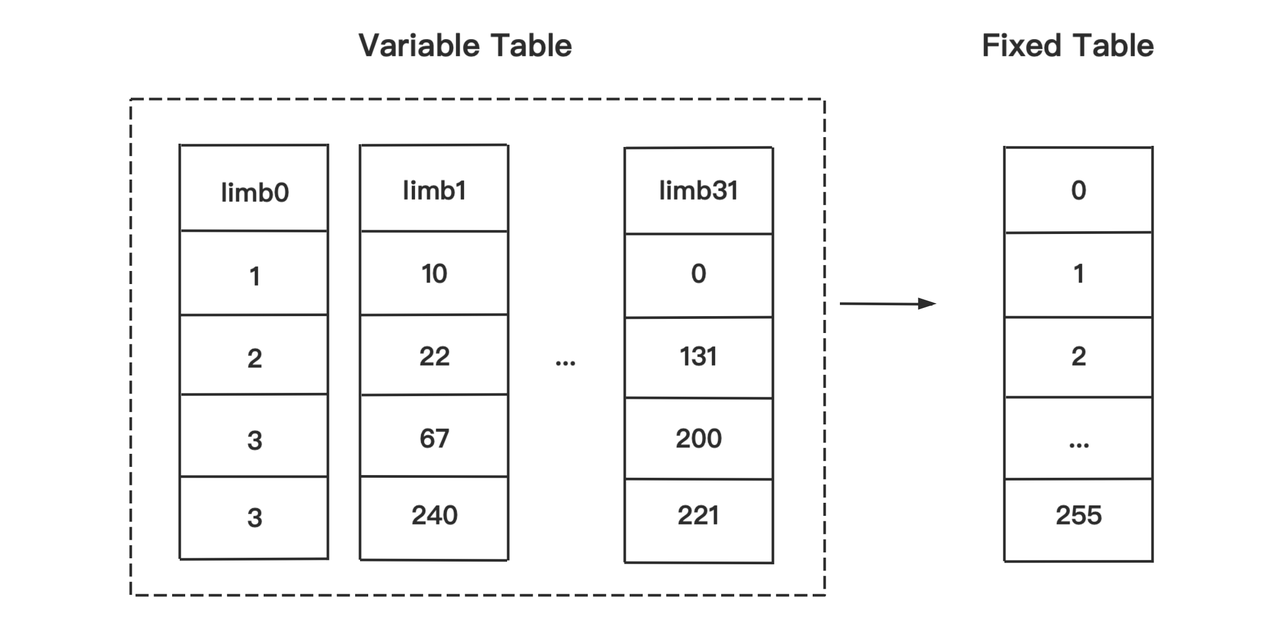
\includegraphics[width=0.8\textwidth]{rangecheck-lookup.png}
    \caption{Fixed/Variable lookup table}
    \label{fig:rangecheck-lookup}
\end{figure}

For numbers greater than 8 bits, break them down to multiple 8-bit limbs and perform Plookup respectively, and then check the constraints of sum and limbs. Take 256-bit as an example,
$\text{integer256} = \text{limb}_0 + \text{limb}_1 \cdot 2^8 + \text{limb}_2 \cdot (2^8)^2 + \text{limb}_3 \cdot (2^8)^3 + \cdots + \text{limb}_{31} \cdot (2^8)^{31}$.

\subsection{Bitwise}

Lookup Arguments are also utilized to implement most of the bitwise operations. The basic lookup table is based on 8 bits, containing three columns, two inputs and one bitwise output, as shown in Table \ref{table:bitwise-lookup}.

\begin{table}[!ht]
    \centering
    \begin{tabular}{|l|l|l|l|}
    \hline
        & \emph{lhs} & \emph{rhs} & \emph{out} \\ \hline
        BitwiseAND table & lhs = 8-bit & rhs = 8-bit & lhs AND rhs \\ \hline
        BitwiseOR table & lhs = 8-bit & rhs = 8-bit & lhs OR rhs \\ \hline
        BitwiseXOR table & lhs = 8-bit & rhs = 8-bit & lhs XOR rhs \\ \hline
    \end{tabular}
    \caption{Bitwise lookup table}
    \label{table:bitwise-lookup}
\end{table}

Bitwise operations larger than 8 bits are broken down into multiple 8-bit operations with Plookup ran on each operation. Take the 32-bit AND of two numbers as an example,
\begin{align*}
a \land b &= (a_0 + a_1\cdot2^8 + a_2 \cdot (2^8)^2 + a_3\cdot(2^8)^3) \land (b_0 + b_1\cdot2^8 + b_2 \cdot (2^8)^2 + b_3\cdot(2^8)^3)\\ &= (a_0 \land b_0) + (a_1 \land b_1)\cdot2^8 + (a_2 \land b_2)\cdot(2^8)^2+(a_3 \land b_3)\cdot(2^8)^3.
\end{align*}

Therefore, for two $n$-bit numbers $a$ and $b$, let $m=n/8$, and $a_i,b_i$ are their limbs, then
\begin{align*}
a \land b &= \sum_{i=0}^{m-1} (2^{8i} \cdot (a_i \land b_i)), \\
a \lor b &= \sum_{i=0}^{m-1} (2^{8i} \cdot (a_i \lor b_i)), \\
a \oplus b &= \sum_{i=0}^{m-1} (2^{8i} \cdot (a_i \oplus b_i)).
\end{align*}

The implementation of NOT is slightly different. The NOT to constrain $a$ is
\[ \neg a + a = 2^{256} - 1. \]

\subsection{Sinsemilla Hash}

We use Halo2 \cite{website:halo2} Sinsemilla Hash scheme.

For detailed design of the hash algorithm and the parameters used below, please refer to Section \ref{sec:key-technologies}.
Following is the main calculation process of Sinsemilla:
\begin{enumerate}
    \item Set the initial value $\mathrm{Acc}_0 = Q$
    \item Perform loop calculation of $i$ from $0$ to $n-1$:
    \[ \mathrm{Acc}_{i+1} = (\mathrm{Acc}_i + P_{m_{i+1}}) + \mathrm{Acc}_i. \]
\end{enumerate}

Now, let $R_i = \mathrm{Acc}_i + P_{m_{i+1}}$, then $\mathrm{Acc}_{i+1} = R_i + \mathrm{Acc}_i$ then according to previous definition, we have
\begin{align*}
\lambda_{1,i} &= \frac {y_{Acc,i} - y_{P,i}}{x_{Acc,i}-x_{P,i}}, \\
x_{R,i} &= \lambda_{1,i}^2 - x_{\text{Acc},i}-x_{P,i}, \\
y_{R,i} &= \lambda_{1,i} (x_{\text{Acc},i} - x_{R,i}) - y_{\text{Acc},i}, \\
\lambda_{2,i} &= \frac {y_{\text{Acc},i} - y_{R,i}}{x_{\text{Acc},i}-x_{R,i}}, \\
x_{\text{Acc},i+1} &= \lambda_{2,i}^2 - x_{\text{Acc},i}-x_{R,i}, \\
y_{\text{Acc},i+1} &= \lambda_{2,i} (x_{\text{Acc},i} - x_{\text{Acc},i+1}) - y_{\text{Acc},i}.
\end{align*}

So, we have constrains as in Table \ref{table:raw-sinsemilla-hash-constraints}.
\begin{table}[!ht]
    \centering
    \begin{tabular}{|c|l|l|}
    \hline
    \emph{Degree} & \emph{Constraints} & \emph{Notes} \\
    \hline
    3 & $q_\text{incomplete-add} \cdot (x_{R,i} + x_{\text{Acc},i} + x_{P,i} - \lambda_{1,i}^2) = 0$
    & $x_{R,i} = \lambda_{1,i}^2 - x_{\text{Acc},i} - x_{P,i}$ \\
    3 & $q_\text{incomplete-add} \cdot (\lambda_{1,i} (x_{\text{Acc},i} - x_{R,i}) - (y_{\text{Acc},i} + y_{R,i})) = 0$
    & $y_{R,i} = \lambda_{1,i} (x_{\text{Acc},i} - x_{R,i}) - y_{\text{Acc},i}$ \\
    3 & $q_\text{incomplete-add} \cdot (\lambda_{1,i} (x_{\text{Acc},i} - x_{P,i}) - (y_{\text{Acc},i} - y_{P,i})) = 0$
    & $\lambda_{1,i} = (y_{\text{Acc},i} - y_{P,i}) / (x_{\text{Acc},i}-x_{P,i})$ \\
    3 & $q_\text{incomplete-add} \cdot (x_{\text{Acc},i+1} + x_{\text{Acc},i} + x_{R,i} - \lambda_{2,i}^2) = 0$
    & $x_{\text{Acc},i+1} = \lambda_{2,i}^2 - x_{\text{Acc},i}-x_{R,i}$ \\
    3 & $q_\text{incomplete-add} \cdot (\lambda_{2,i} (x_{\text{Acc},i} - x_{\text{Acc},i+1}) - (y_{\text{Acc},i} + y_{\text{Acc},i+1})) = 0$
    & $y_{\text{Acc},i+1} = \lambda_{2,i} (x_{\text{Acc}_,i} - x_{\text{Acc},i+1}) - y_{\text{Acc},i}$ \\
    3 & $q_\text{incomplete-add} \cdot (\lambda_{2,i} (x_{\text{Acc},i} - x_{R,i}) - (y_{\text{Acc},i} - y_{R,i}) ) = 0$
    & $\lambda_{2,i} = (y_{\text{Acc},i} - y_{R,i}) / (x_{\text{Acc}_i}-x_{R,i})$ \\
    \hline
    \end{tabular}
    \caption{Sinsemilla Hash constraints}
    \label{table:raw-sinsemilla-hash-constraints}
\end{table}
\begin{align*}
    & \lambda_{2,i} = \frac {y_{\text{Acc},i} - y_{R,i}}{x_{\text{Acc},i}-x_{R,i}} \\
    \implies & y_{\text{Acc},i} - y_{R,i} = \lambda_{2,i} (x_{\text{Acc},i}-x_{R,i}), \\
    & y_{R,i} = \lambda_{1,i} (x_{\text{Acc},i} - x_{R,i}) - y_{\text{Acc},i} \\
    \implies & y_{\text{Acc},i} - (\lambda_{1,i} (x_{\text{Acc},i} - x_{R,i}) - y_{\text{Acc},i}) = \lambda_{2,i} (x_{\text{Acc},i}-x_{R,i}) \\
    \implies & 2y_{\text{Acc},i} = (\lambda_{1,i} + \lambda_{2,i}) (x_{\text{Acc},i}-x_{R,i}).
\end{align*}

Therefore, the check for $\lambda_{2,i} = (y_{\text{Acc}_i} - y_{R,i})/(x_{\text{Acc}_i}-x_{R,i})$ can be replaced by
\[ q_\text{incomplete-add} \cdot (\lambda_{2,i} (x_{\text{Acc},i} - x_{R,i}) - (y_{\text{Acc},i} - y_{R,i}) ) = 0, \]

then
\[ q_\text{incomplete-add} \cdot ((\lambda_{2,i} + \lambda_{1,i}) (x_{\text{Acc},i} - x_{R,i}) - 2y_{\text{Acc},i}) = 0. \]

We haven't used $y_{R,i}$ of $R_i = \{x_{R,i}, y_{R,i}\}$ in the second step of checking for $\mathrm{Acc}_{i+1} = R_i + \mathrm{Acc}_i$. Therefore, remove the constraint on $y_{R,i}$ in the first step and the entire constraint develop into what is displayed in Table \ref{table:simplified-sinsemilla-hash-constraints}.

\begin{table}[!ht]
    \centering
    \begin{tabular}{|c|l|l|}
        \hline
        \emph{Degree} & \emph{Constraints} & \emph{Notes} \\
        \hline
        3 & $q_\text{incomplete-add} \cdot (x_{R,i} + x_{\text{Acc},i} + x_{P,i} - \lambda_{1,i}^2) = 0$
        & $x_{R,i} = \lambda_{1,i}^2 - x_{\text{Acc},i} - x_{P,i}$ \\
        3 & $q_\text{incomplete-add} \cdot (\lambda_{1,i} (x_{\text{Acc},i} - x_{P,i}) - (y_{\text{Acc},i} - y_{P,i})) = 0$
        & $\lambda_{1,i} = (y_{\text{Acc},i} - y_{P,i}) / (x_{\text{Acc},i}-x_{P,i})$ \\
        3 & $q_\text{incomplete-add} \cdot (x_{\text{Acc},i+1} + x_{\text{Acc},i} + x_{R,i} - \lambda_{2,i}^2) = 0$
        & $x_{\text{Acc},i+1} = \lambda_{2,i}^2 - x_{\text{Acc},i}-x_{R,i}$ \\
        3 & $q_\text{incomplete-add} \cdot (\lambda_{2,i} (x_{\text{Acc},i} - x_{\text{Acc},i+1}) - (y_{\text{Acc},i} + y_{\text{Acc},i+1})) = 0$
        & $y_{\text{Acc},i+1} = \lambda_{2,i} (x_{\text{Acc},i} - x_{\text{Acc},i+1}) - y_{\text{Acc},i}$ \\
        3 & $q_\text{incomplete-add} \cdot ((\lambda_{2,i} + \lambda_{1,i}(x_{\text{Acc},i} - x_{R,i}) - 2y_{\text{Acc},i} ) = 0$
        & $\lambda_{2,i} = (y_{\text{Acc},i} - y_{R,i}) / (x_{\text{Acc},i}-x_{R,i})$ \\
        \hline
    \end{tabular}
    \caption{Simplified Sinsemilla Hash constraints}
    \label{table:simplified-sinsemilla-hash-constraints}
\end{table}

\subsection{Comparison}

Range Check is used to perform \verb|GTE| comparison, using Cairo's scheme \cite{cryptoeprint:2021/1063}.

On a circuit level, we only need to support 3 comparisons: \verb|EQ|, \verb|GTE| and \verb|NEQ|. We will perform 256-bit Range Check for two numbers to be compared, and then perform a 256-bit Range Check for the difference between two numbers.

\verb|EQ| checks the equality of two 256-bit numbers $a$ and $b$. The constraint is $a-b=0$.

\verb|NEQ| checks the inequality of two 256-bit numbers $a$ and $b$. The constraint is $(a-b)\cdot(a-b)^{-1}=1$.

\verb|GTE| checks whether two 256-bit numbers $a$ and $b$ satisfy $a \geq b$.

First, use Range Check to constrain each number in 256 bits, and then compare them according to the difference. If the difference exceeds 256 bits, it means that they don't satisfy $a \geq b$. The constraint pseudo code is
\begin{lstlisting}[language=Rust]
range_check(integer256_a, range256bit)
range_check(integer256_b, range256bit)
let diff = integer256_a - integer256_b
range_check(diff, range256bit)
\end{lstlisting}

We can combine \verb|GTE| and \verb|NEQ| with bitwise operations to perform other comparisons, listed in Table \ref{table:comparison-level}.
\begin{table}[!ht]
    \centering
    \begin{tabular}{|l|l|}
    \hline
        \emph{Application level} & \emph{Circuit level} \\ \hline
        $a \ge b$ & a \verb|GTE| b \\
        $a \le b$ & b \verb|GTE| a \\
        $a > b$ & (a \verb|GTE| b) \&\& (a \verb|NEQ| b) \\
        $a < b$ & (b \verb|GTE| a) \&\& (b \verb|NEQ| a) \\ \hline
    \end{tabular}
    \caption{Comparison level}
    \label{table:comparison-level}
\end{table}

\subsection{Signature}

We support two different signature schemes, ECDSA \cite{Johnson99theelliptic} and Schnorr \cite{jofc-1991-14302}.

\subsubsection{ECDSA Signature}

The hash function we choose is Sinsemilla Hash, which is the same function used in signature generation. With the following notations:
\begin{itemize}
    \item $(r, s)$ is the signature.
    \item $m$ is the message to verify.
    \item $Q(Q_x, Q_y)$ is the public-key curve point.
    \item $h$ is the hash result of $m$.
    \item $G$ is the elliptic curve base point.
    \item $n$ is the order of $G$.
    \item $\mathcal{O}$ is the identity element.
    \item $L_n$ is the bit length of $n$.
\end{itemize}

The constraints are the following:
\begin{enumerate}
    \item Check that $Q$ is not equal to $\mathcal{O}$.
    \item Check that $Q$ lies on the curve, which means: $Q_y^2 = Q_x^3+\alpha Q_x + \beta$.
    \item Check that $nQ = \mathcal{O}$.
    \item Check that $r$ and $s$ are in $[1, n-1]$.
    \item Let $z$ be the leftmost $L_n$ bits of $h$ (we use Sinsemilla Hash builtin circuit to check $h \equiv \mathrm{HASH}(m)$).
    \item Calculate $u_1 = zs^{-1} \bmod n$ and $u_2 = rs^{-1} \bmod n$.
    \item Calculate curve point $(x_1,y_1) = u_1 G + u_2 Q$, check $(x_1, y_1) \ne \mathcal{O}$.
    \item Check that $r \equiv x_1 \pmod n$.
\end{enumerate}

\subsubsection{Schnorr Signature}

Schnorr signature is known for its simplicity, Bitcoin used Schnorr signature as well. The hash function we choose is Sinsemilla Hash. With the following notations:
\begin{itemize}
    \item $(s, e)$ is the signature.
    \item $m$ is the message to verify, it is represented as list of finite bit strings.
    \item $h$ is the hash result of $m$.
    \item $g$ is the generator.
    \item $y$ is the public verification key.
\end{itemize}

The constraints are the following:
\begin{enumerate}
    \item Check $r_v = g^s y^e$.
    \item Check $e_v = \mathrm{Hash}(r_v \mathbin{||} m)$, where $||$ denotes concatenation, $r_v$ is represented as a bit string (Like above, we use Sinsemilla Hash builtin circuit to check it).
    \item Check that $e_v \equiv e$.
\end{enumerate}

\vspace{3mm}
Schnorr signature also supports Multi-Signatures \cite{cryptoeprint:2018/068}, which could provide more security. Given
\begin{itemize}
    \item A list of public keys $L = \{X_1, X_2, \ldots, X_n\}$.
    \item An aggregated public key $X = \prod_{i=1}^n H(L, X_i) X_i$.
    \item A message $m$.
    \item A signature $(R, s)$.
    \item A list of random numbers $R_i = g^{r_i}$ and $R=\prod_{i=1}^n R_i$.
\end{itemize}

The constraints are the following:
\begin{enumerate}
    \item Check $c = \mathrm{Hash}(X, R, m)$ (As always, this can be done in Hash builtin circuit).
    \item Check $u = c X$.
    \item Check $s G \equiv R + u$.
\end{enumerate}


    \section{Storage Module} \label{sec:storage-module}

\subsection{Verkle Tree Structure}

We use Verkle Tree to store storage data. The width of Verkle Tree is 256, and the nodes are divided into two types: InternalNode and LeafNode. We use KZG commitments for vector commitments. The order $n = 2^{251} + 17 \cdot 2^{192} + 1$ of the curve we selected is a 252-bit prime number, so we can only make safe commitments for 251-bit values. Each key consists of 32-bytes. The structure of Verkle Tree is shown in Figure \ref{fig:verkle-tree-struct}.
\begin{figure}[!ht]
    \centering
    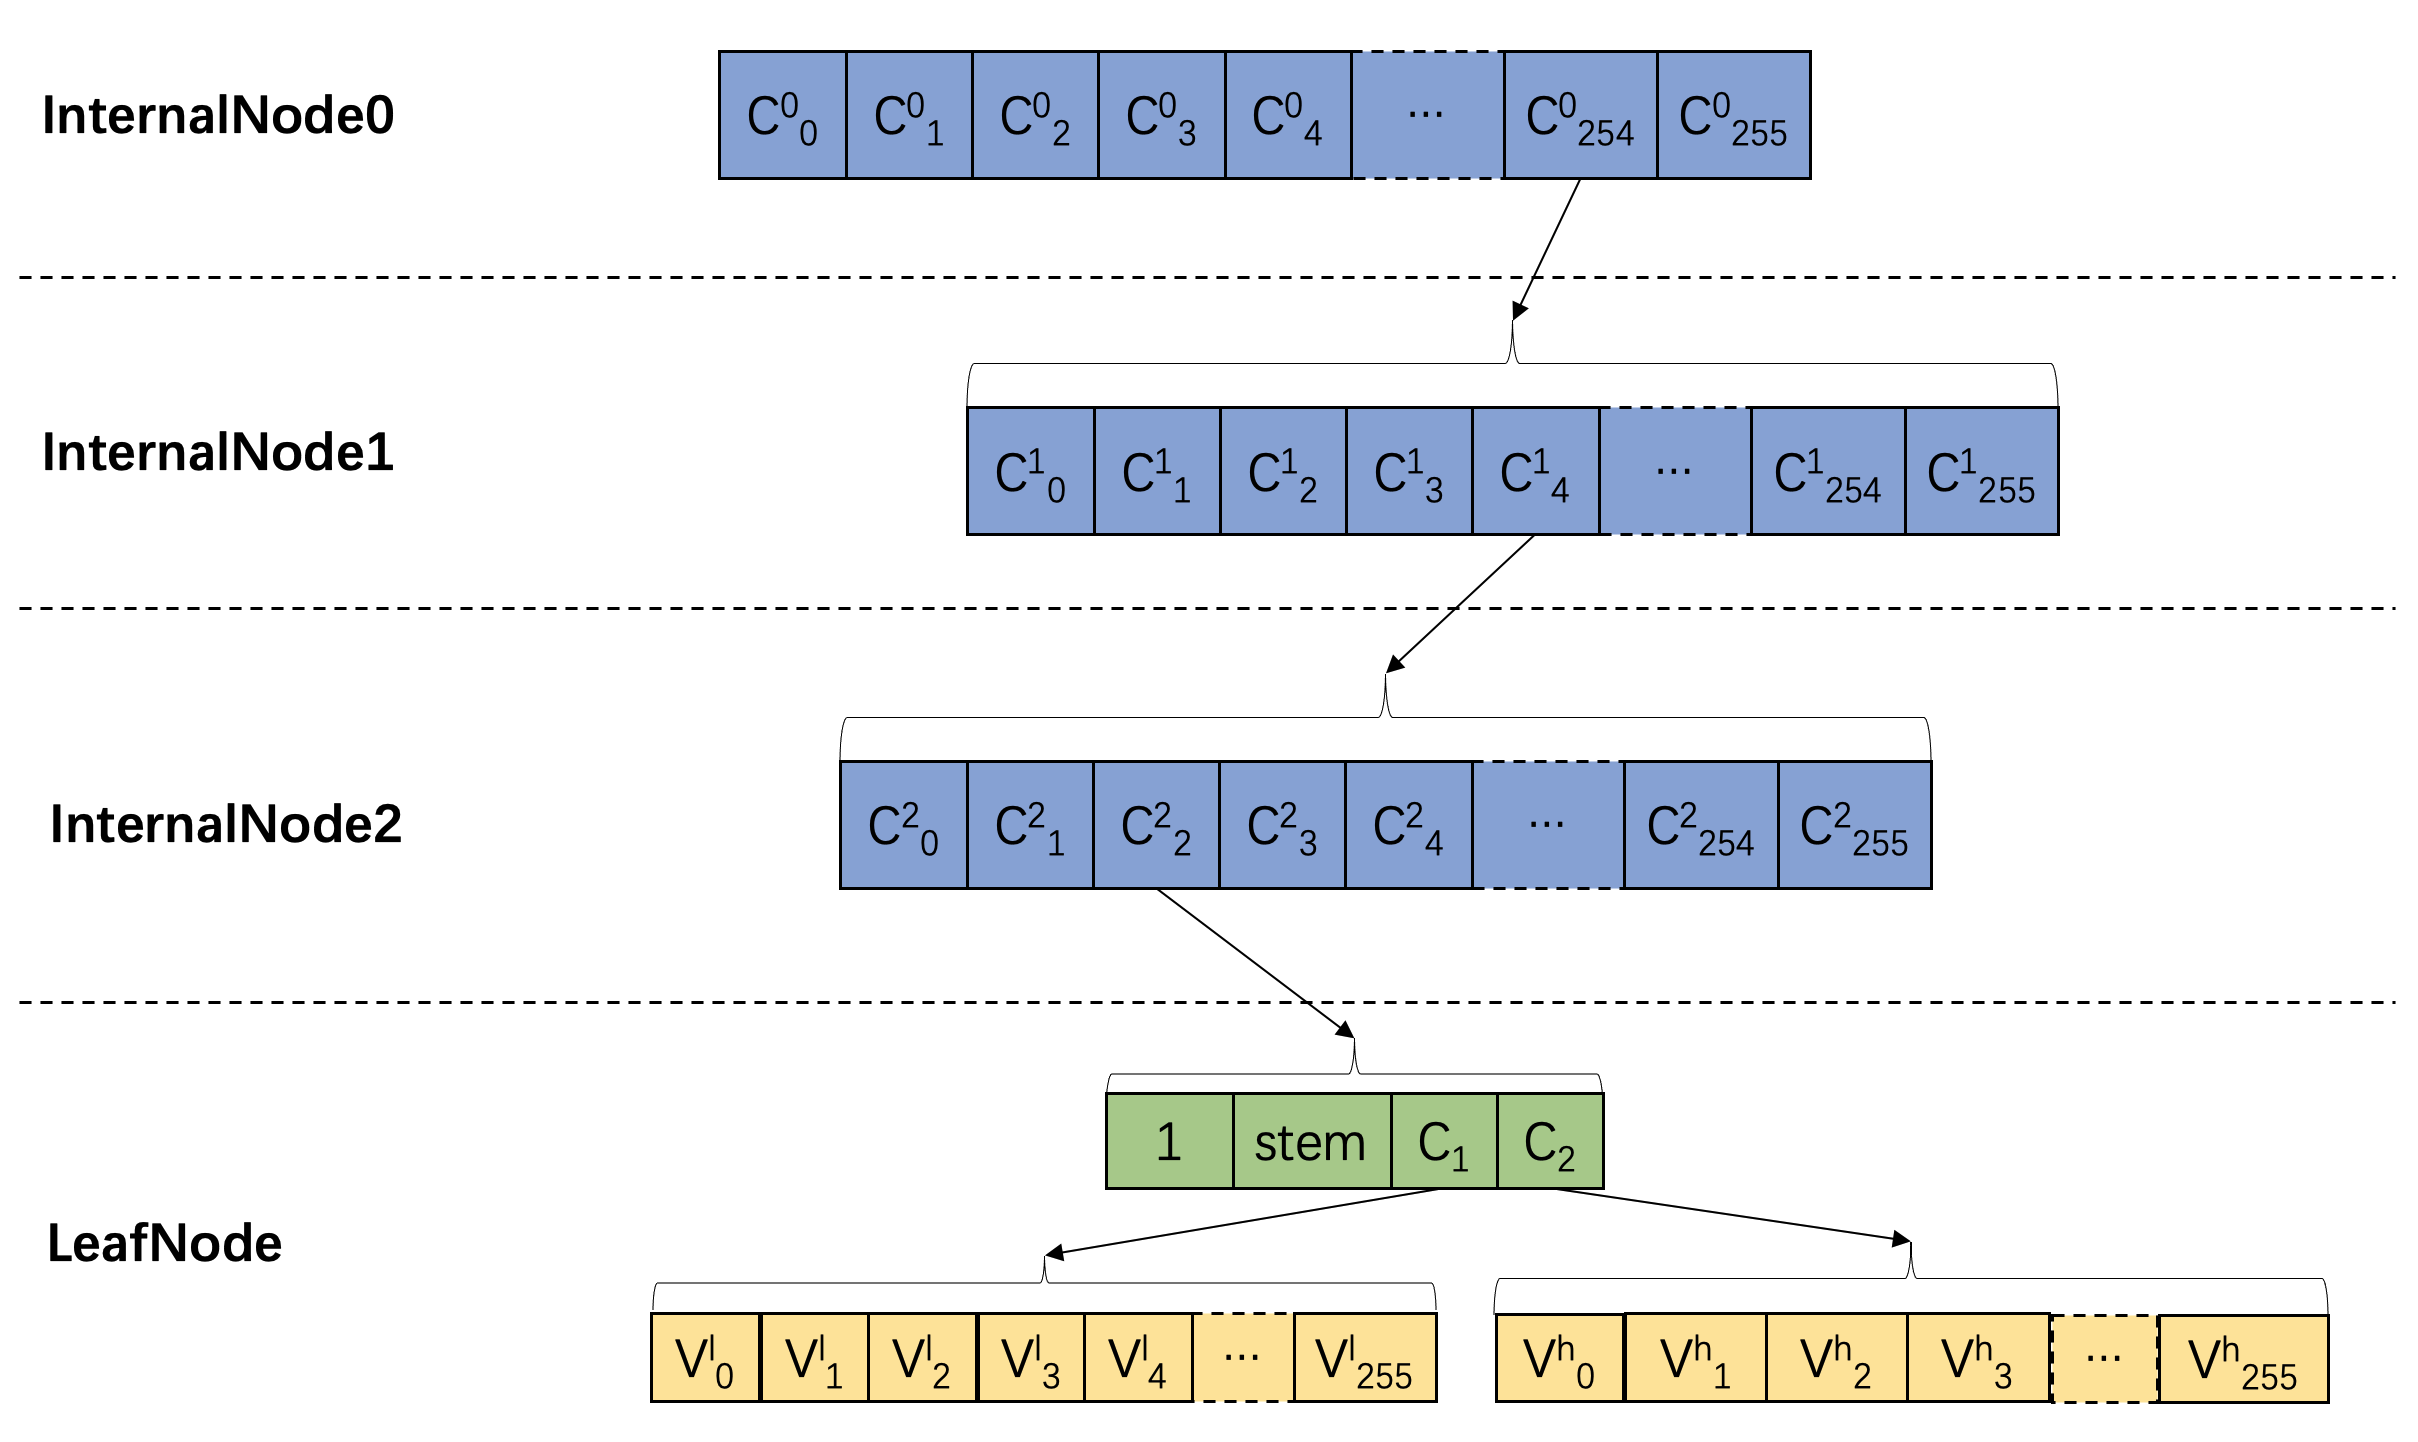
\includegraphics[width=0.8\textwidth]{storage/verkle_struct.png}
    \caption{Structure of Verkle Tree}
    \label{fig:verkle-tree-struct}
\end{figure}

For LeafNode, each value $V_i$ is 32-bytes. To make commitments to vector $\{V_i\}$, we split each value $V_i$ into two 16-byte values $V^l_i$ and $V^h_i$, and make commitments to $\{V^l_i\}$ and $\{V^h_i\}$ as $C_1 = \mathrm{Commit}(V^l_0, V^l_1, V^l_2, \ldots, V^l_{255})$, $C_2 = \mathrm{Commit}(V^h_0, V^h_1, V^h_2, \ldots, V^h_{255})$ respectively. It should especially be noted that the node will not be deleted at the data level, but use the 128th bit of $V^l_i$ as the marker bit of the deleted node. If the 128th bit of $V^l_i$ is set to 1, it means the node has been deleted. The commitment of LeafNode is composed of flag bit 1, stem and two sub-commitments $C_1$, $C_2$, i.e.
\[ C = \mathrm{Commit}(1, \mathrm{stem}, C_1, C_2). \]
The commitment to InternalNode is relatively simpler that the commitment to empty node is 0 and if the node is non-empty, just directly make commitments to all 256 commitment values, namely
\[ C = \mathrm{Commit}(C_0, C_1, C_2, \ldots, C_{255}). \]

\subsection{Verkle Tree Vector Commitment}

Define that the random number selected by SRS is $R$. The Lagrange basis for evaluating polynomials of 256 points is $\delta_i$, i.e.
\[ \delta_i = \prod_{\substack{k=0 \\ k\neq i}}^{255} \frac{R - k}{i - k}. \]
Commitment to the InternalNode:
\[ C = \mathrm{Commit}(C_0, C_1, C_2, \ldots, C_{255}) = \sum_{i=0}^{255}C_i\delta_i. \]
Two child commitments to the LeafNode:
\begin{gather*}
    C_1 = \mathrm{Commit}(V^l_0, V^l_1, V^l_2, \ldots, V^l_{255}) = \sum_{i=0}^{255}V^l_i\delta_i, \\
    C_2 = \mathrm{Commit}(V^h_0, V^h_1, V^h_2, \ldots, V^h_{255}) = \sum_{i=0}^{255}V^h_i\delta_i.
\end{gather*}
Commitment to the LeafNode:
\begin{gather*}
    C = \mathrm{Commit}(1, \mathrm{stem}, C_1, C_2) = \delta_0 + \mathrm{stem} \cdot \delta_1 + C_1\delta_2 + C_2\delta_3+\sum_{i=3}^{255}C_i\delta_i, \\
    C_i = 0, \quad \forall i \ge 3.
\end{gather*}

\subsection{Design of Verkle Tree Constraints}

Our constraints are designed for a key change, when the key changes, we constrain the node changes of the corresponding path. When the value of the constraint key changes from $V_1$ to $V_2$, the root of Verkle Tree should change from $\text{root}_1$ to $\text{root}_2$.
\begin{itemize}
    \item the value of key $V_1$ corresponds to the root of storage as $\text{root}_1$;
    \item the value of key $V_2$ corresponds to the root of storage as $\text{root}_2$.
\end{itemize}

Since we do not delete keys at data level, we're adding a ``deletion flag'', Verkle Tree modification actually has only two kinds of operations, update and insert.

\subsubsection{Constraints for Node Update}

Figure \ref{fig:upgrade-constraint} shows the value update constraint schematic.
\begin{figure}[!ht]
    \centering
    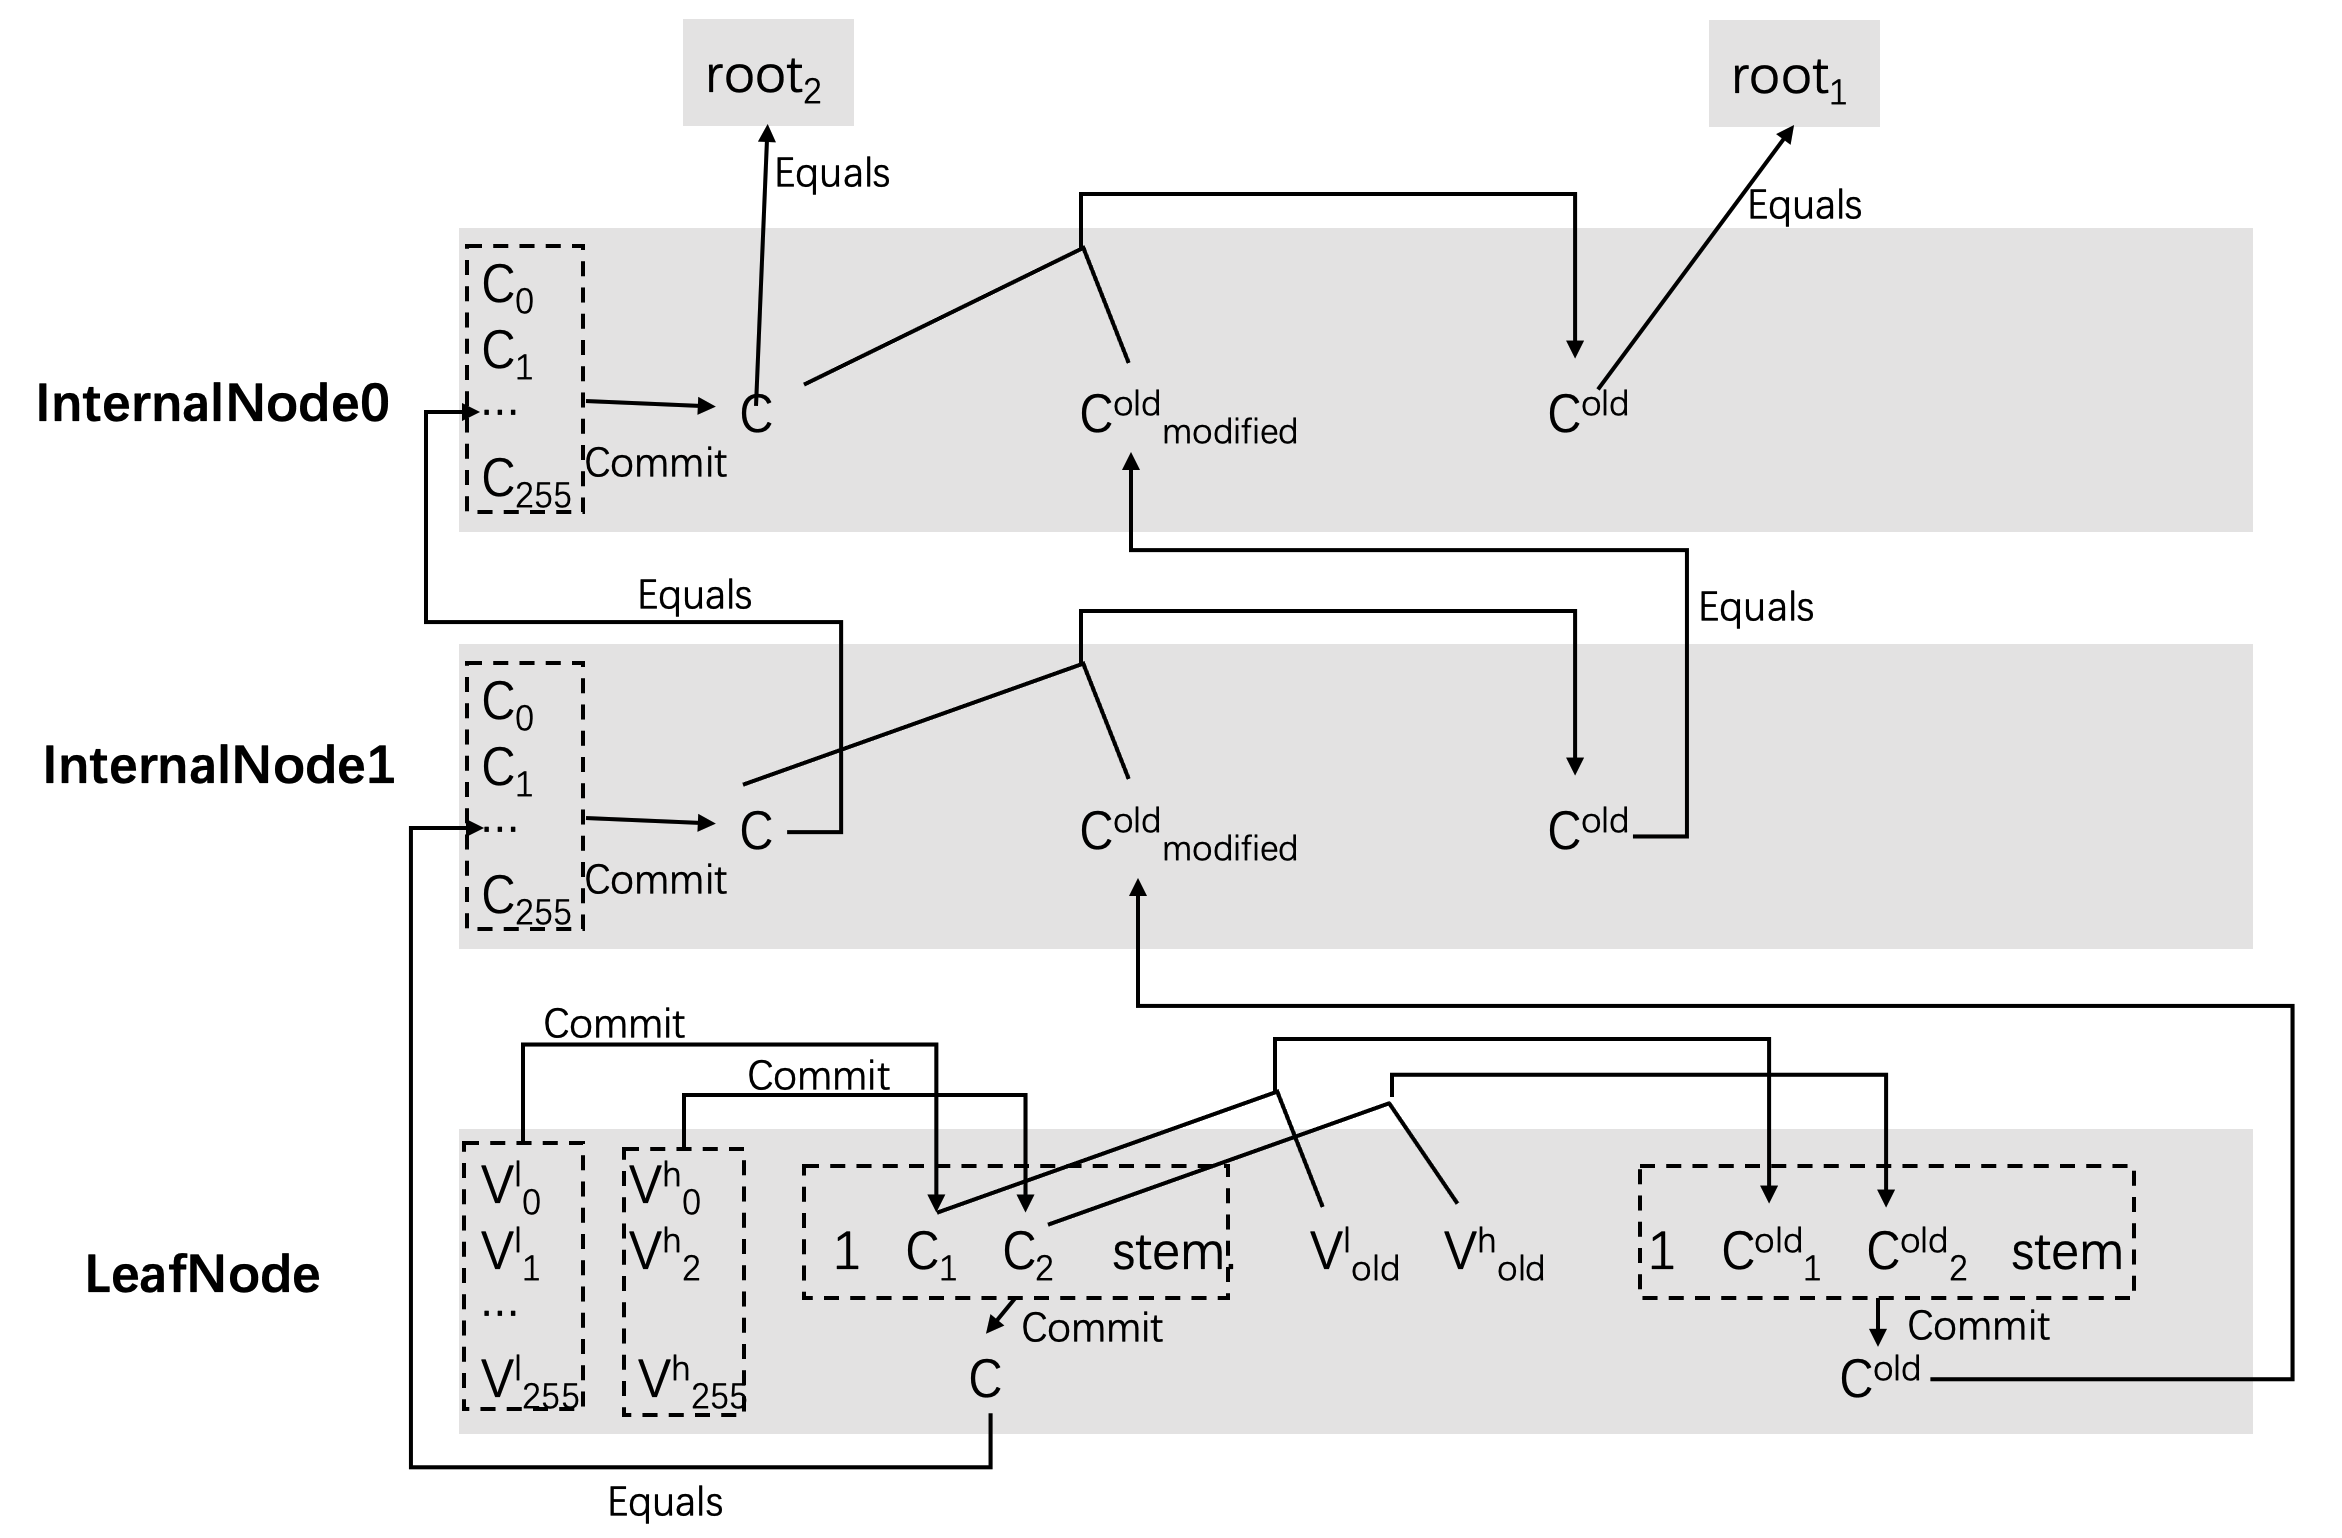
\includegraphics[width=0.8\textwidth]{storage/upgrade_constraint.png}
    \caption{Verkle Tree Update Constraint Schematic}
    \label{fig:upgrade-constraint}
\end{figure}

As for the path related to the updated value, trace table records the completed updated value, i.e.\ $\{V^l_i\}, \{V^h_i\}$ of LeafNode and $\{C_i\}$ of InternalNode. The value before update is represented as $V^l_\text{old}$ and $V^h_\text{old}$ in LeafNode, $C^\text{old}_\text{modified}$ in InternalNode.

In LeafNode, $\{V^l_i\}$ is committed to $C_1$ and $\{V^h_i\}$ is committed to $C_2$. According to the commitment protocol, we can compute the pre-update commitment $C^\text{old}_1$ using $C_1$ and $V^l_\text{old}$, and compute the pre-update commitment $C^\text{old}_2$ using $C_2$ and $V^h_\text{old}$. Finally make a commitment to LeafNode to get the updated commitment $C$ and the commitment before update $C^\text{old}$, and also constrain $C$ to be equal to the commitment of the change line of parent, $C^\text{old}$ to be equal to the pre-change commitment of the change line of parent.

In InternalNode, commit $\{C_i\}$ to $C$, and then the commitment protocol utilizes $C$ and $C^\text{old}_\text{modified}$ to calculate the pre-updated commitment $C^\text{old}$ of this node. Constrain them to be equal to the corresponding values in parent. If the node is on the top-level, constrain $C = \text{root}_2$, $C^\text{old} = \text{root}_1$.

\subsubsection{Constraints for Node Insert}

We have three cases for inserting nodes:
\begin{enumerate}
    \item The node is inserted at the position of EmptyNode in InternalNode.
    \item The node is inserted into the LeafNode position of the InternalNode, and the newly inserted LeafNode has the same stem as the LeafNode at the original position.
    \item The node is inserted into the LeafNode position of the InternalNode, and the newly inserted LeafNode has the different stem from the LeafNode at the original position.
\end{enumerate}

There are no differences between the first/second cases and the constraint logic of node update, which will not be discussed again here. For the third case of inserting a node, the logic of inserting is shown in Figure \ref{fig:insert-constraint-1}.
\begin{figure}[!ht]
    \centering
    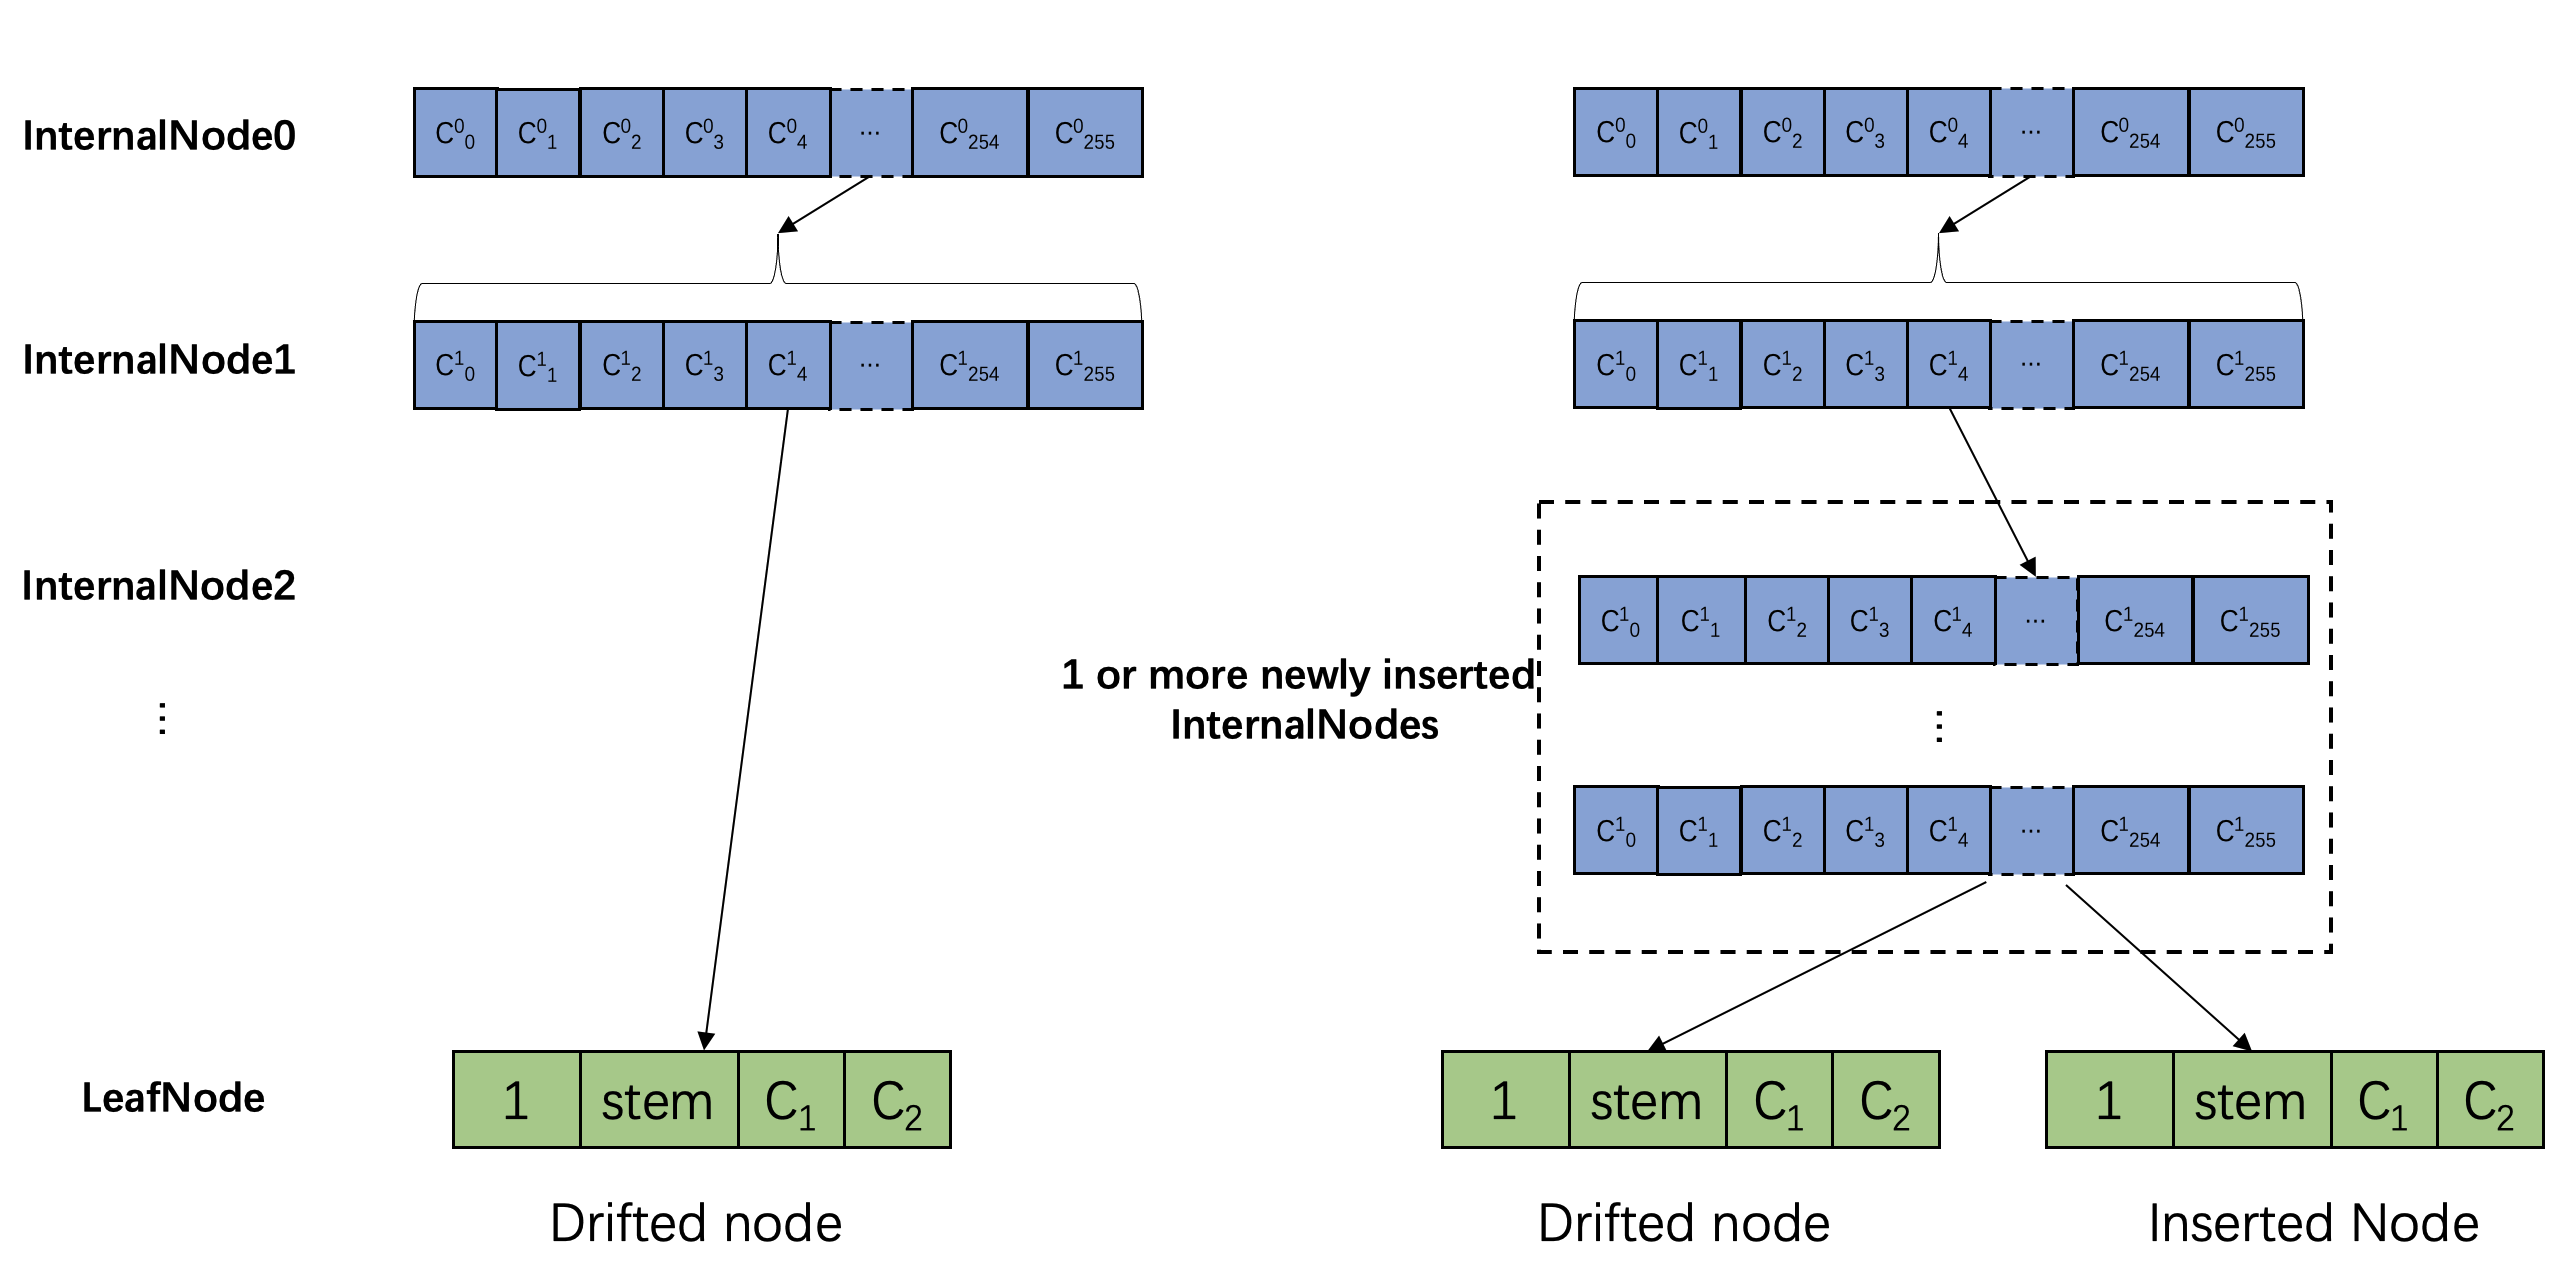
\includegraphics[width=0.8\textwidth]{storage/insert_node1.png}
    \caption{Verkle Tree Update Constraint Schematic}
    \label{fig:insert-constraint-1}
\end{figure}

The position of the newly inserted node in InternalNode has been occupied by a LeafNode, called DriftedNode. Meanwhile, the stem of the newly inserted node is different from that of the original DriftedNode. At this time, one or more InternalNodes need to be added until the paths of the newly inserted LeafNode and the DriftedNode are on different nodes of the InternalNode. Finally, insert the DriftedNode and the newly inserted LeafNode.

In this case, we are supposed to perform constrains to DriftedNode in addition to insert full paths of the node when constraining as Figure \ref{fig:insert-constraint-2}.
\begin{figure}[!ht]
    \centering
    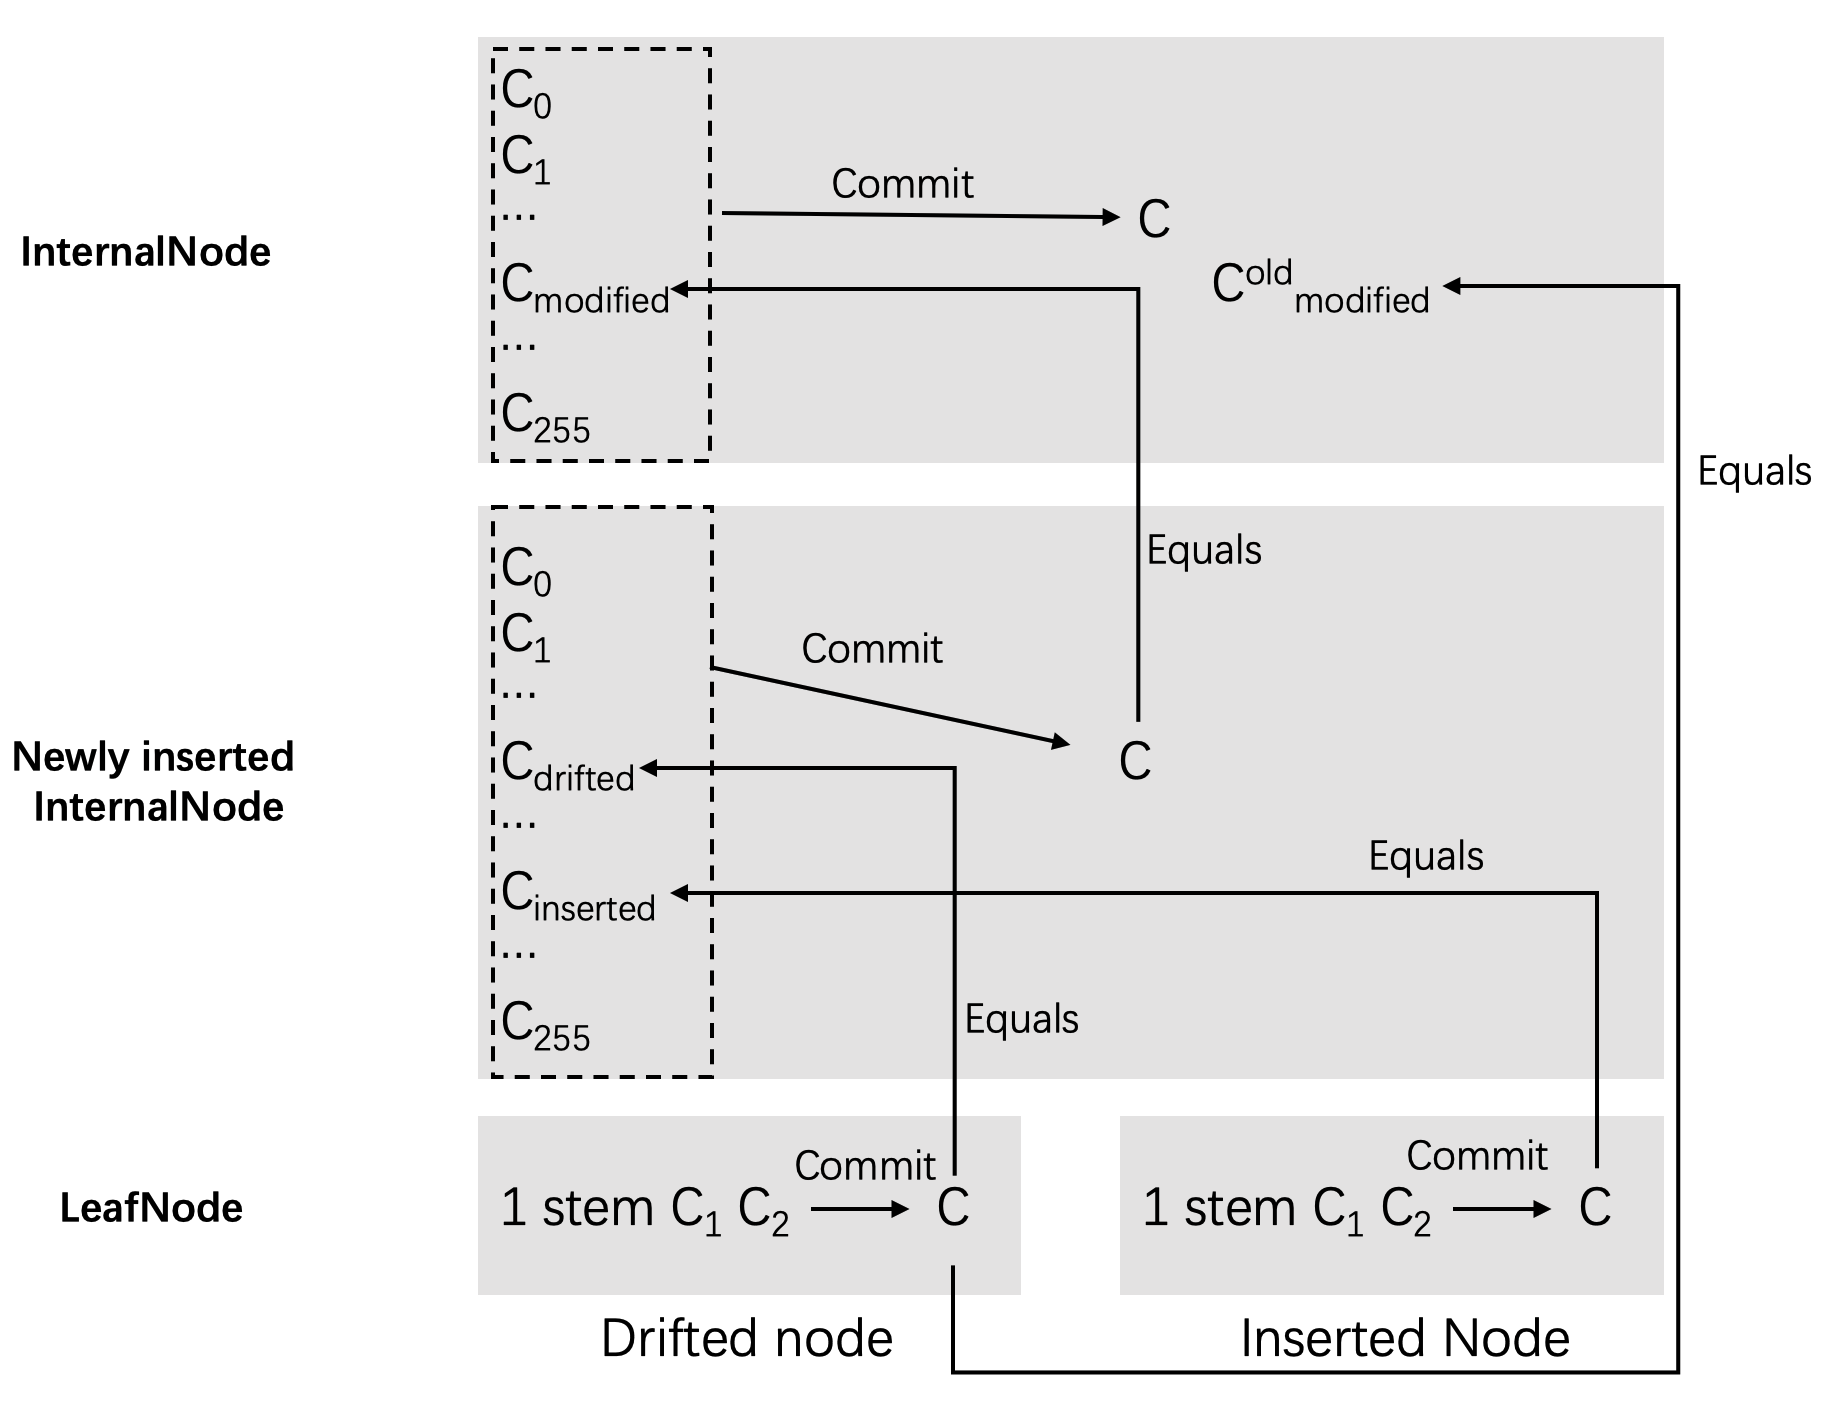
\includegraphics[width=0.8\textwidth]{storage/insert_node2.png}
    \caption{Verkle Tree update constraint schematic}
    \label{fig:insert-constraint-2}
\end{figure}

\subsection{Verkle Tree Trace Table and Constraints}

\subsubsection{Constraints for InternalNode}

Figure \ref{table:trace-table-for-internal-node} shows the structure of the trace section of InternalNode.

\begin{table}[!ht]
    \centering
    \resizebox{\textwidth}{!}{
    \begin{tblr}{
        colspec = {|c|c|c|c|c|c|c|c|c|},
        row{1} = {bg=lightgray},
        hline{1,9} = {1pt,solid},
        hline{5,6} = {red,dashed},
        hline{8} = {solid},
        vline{1,10} = {5}{red},
        vline{1,10} = {4,6}{dashed},
    }
        data & data\_aux & pre\_data & pre\_data\_aux & is\_modified & basis & acc\_c & acc\_c\_aux & acc\_diff \\
        $C_0$ & 0 & 0 & 0 & 0 & $\delta_0$ & $C_0 \delta_0$ & 0 & 0 \\
        $C_1$ & 0 & 0 & 0 & 0 & $\delta_1$ & $C_0 \delta_0 + C_1 \delta_1$ & 0 & 0 \\
        $\cdots$ & $\cdots$ & $\cdots$ & $\cdots$ & $\cdots$ & $\cdots$ & $\cdots$ & $\cdots$ & $\cdots$ \\
        $C_k$ & 0 & $C_\text{old\_k}$ & 0 & 1 & $\delta_k$ & $\sum_{i=0}^kC_i\delta_i$ & 0 & $-C_k \cdot \delta_k+C^\text{old}_k\delta_k$ \\
        $\cdots$ & $\cdots$ & $\cdots$ & $\cdots$ & $\cdots$ & $\cdots$ & $\cdots$ & $\cdots$ & $\cdots$ \\
        $C_{255}$ & 0 & 0 & 0 & 0 & $\delta_{255}$ & $\sum_{i=0}^{255}C_i\delta_i$ & 0 & $-C_k \cdot \delta_{255}+C^\text{old}_k\delta_k$ \\
        $C_\text{curr}$ & $C_\text{old\_curr}$ & 0 & 0 & 0 & 0 & 0 & 0 & 0
    \end{tblr}
    }
    \resizebox{\textwidth}{!}{
    \begin{tblr}{
        colspec = {|c|c|c|c|c|c|c|},
        row{1} = {bg=lightgray},
        hline{1,9} = {1pt,solid},
        hline{5,6} = {red,dashed},
        hline{8} = {solid},
        vline{1,10} = {5}{red},
        vline{1,10} = {4,6}{dashed},
    }
        acc\_diff\_aux & is\_leaf & is\_drifted & is\_child\_row & is\_first\_child\_row & modified\_rlc & modified\_rlc\_mult \\
        0 & 1 & 0 & 1 & 1 & 0 & $R$ \\
        0 & 0 & 0 & 1 & 0 & 0 & $R$ \\
        $\cdots$ & $\cdots$ & $\cdots$ & $\cdots$ & $\cdots$ & $\cdots$ & $\cdots$ \\
        0 & 0 & 0 & 1 & 0 & $C_kR+C_\text{old\_k}R^2$ & $R$ \\
        $\cdots$ & $\cdots$ & $\cdots$ & $\cdots$ & $\cdots$ & $\cdots$ & $\cdots$ \\
        0 & 0 & 0 & 1 & 0 & $C_kR+C_\text{old\_k}R^2$ & $R^3$ \\
        0 & 1 & 0 & 0 & 0 & $C_kR+C_\text{old\_k}R^2$ & $R^3$
    \end{tblr}
    }
    \caption{Trace table for InternalNode}
    \label{table:trace-table-for-internal-node}
\end{table}

\begin{table}[!ht]
    \centering
    \resizebox{\textwidth}{!}{
    \begin{tblr}{
        colspec = {|c|c|c|c|c|c|c|c|c|},
        row{1} = {bg=lightgray},
        hline{1,9} = {1pt,solid},
        hline{5,6} = {red,dashed},
        hline{8} = {solid},
        vline{1,10} = {5}{red},
        vline{1,10} = {4,6}{dashed},
    }
        data & data\_aux & pre\_data & pre\_data\_aux & is\_modified & basis & acc\_c & acc\_c\_aux & acc\_diff \\
        $V^l_0$ & $V^h_0$ & 0 & 0 & 0 & $\delta_0$ & $V^l_0 \delta_0$ & $V^h_0 \delta_0$ & 0 \\
        $V^l_1$ & $V^h_1$ & 0 & 0 & 0 & $\delta_1$ & $V^l_0 \delta_0 + V^l_1 \delta_1$ & $V^h_0 \delta_0+V^h_1 \delta_1$ & 0 \\
        $\cdots$ & $\cdots$ & $\cdots$ & $\cdots$ & $\cdots$ & $\cdots$ & $\cdots$ & $\cdots$ & $\cdots$ \\
        $V^l_k$ & $V^h_k$ & $V^l_\text{old\_k}$ & $V^h_\text{old\_k}$ & 1 & $\delta_k$ & $\sum^k_0 V^l_i \delta_i$ & $\sum^k_0V^h_i \delta_i$ & \tiny{$-V^l_k \delta_k+V^l_\text{old\_k} \delta_k$} \\
        $\cdots$ & $\cdots$ & $\cdots$ & $\cdots$ & $\cdots$ & $\cdots$ & $\cdots$ & $\cdots$ & $\cdots$ \\
        $V^l_{255}$ & $V^h_{255}$ & 0 & 0 & 0 & $\delta_{255}$ & $\sum^{255}_0 V^l_i \delta_i$ & $\sum^{255}_0V^h_i \delta_i$ & \tiny{$-V^l_k \delta_k+V^l_\text{old\_k} \delta_k$} \\
        1 & stem & $C_1$ & $C_2$ & $C_\text{old\_1}$ & $C_\text{old\_2}$ & $C_\text{curr}$ & $C_\text{old\_curr}$ & 0 \\
    \end{tblr}
    }
    \resizebox{\textwidth}{!}{
    \begin{tblr}{
        colspec = {|c|c|c|c|c|c|c|},
        row{1} = {bg=lightgray},
        hline{1,9} = {1pt,solid},
        hline{5,6} = {red,dashed},
        hline{8} = {solid},
        vline{1,10} = {5}{red},
        vline{1,10} = {4,6}{dashed},
    }
        acc\_diff\_aux & is\_leaf & is\_drifted & is\_child\_row & is\_first\_child\_row & modified\_rlc & modified\_rlc\_mult \\
        0 & 1 & 0 & 1 & 1 & 0 & $R$ \\
        0 & 1 & 0 & 1 & 0 & 0 & $R$ \\
        $\cdots$ & $\cdots$ & $\cdots$ & $\cdots$ & $\cdots$ & $\cdots$ & $\cdots$ \\
        $-V^h_k \delta_k+V^h_\text{old\_k} \delta_k$ & 1 & 0 & 1 & 0 & 0 & $R$ \\
        $\cdots$ & $\cdots$ & $\cdots$ & $\cdots$ & $\cdots$ & $\cdots$ & $\cdots$ \\
        $-V^h_k \delta_k+V^h_\text{old\_k} \delta_k$ & 1 & 0 & 1 & 0 & 0 & $R$ \\
        0 & 1 & 0 & 0 & 0 & 0 & $R$ \\
    \end{tblr}
    }
    \caption{Trace table for LeafNode}
    \label{table:trace-table-for-leaf-node}
\end{table}


Each node is divided into 257 rows, of which the first 256 rows are \verb|child_row|s, and the last row is \verb|final_row|.

In \verb|child_row|s:
\begin{itemize}
    \item \verb|data|: Polynomial commitment of the child node;
    \item \verb|is_modified|: Whether the row has been updated;
    \item \verb|pre_data|: Value before the row is updated, or 0 if it is not updated;
    \item \verb|basis|: Lagrange basis;
    \item \verb|acc_c|: Cumulative value of evaluating the committed polynomials, and the value of the column in the last row is the polynomial commitment of the node;
    \item \verb|acc_diff|: Difference between the committed polynomial evaluation before update and the committed polynomial evaluation after update;
    \item \verb|is_leaf|: Whether it's a LeafNode;
    \item \verb|is_first_child_row|: Whether it's the first \verb|child_row|.
\end{itemize}

In \verb|final_row|:
\begin{itemize}
    \item \verb|data|: $C_\text{curr}$, polynomial commitment of the node;
    \item \verb|data_aux|: $C_\text{old\_curr}$, polynomial commitment of the node before update.
\end{itemize}

Accumulate evaluations of constraint polynomials:
\begin{align*}
    & \mathrm{is\_child\_row}_i \cdot (1-\mathrm{is\_modified}_i) \cdot \mathrm{pre\_data}_i=0, \\
    & \mathrm{is\_child\_row}_i \cdot (1-\mathrm{is\_first\_row}_i) \cdot (\mathrm{acc\_c}_i-\mathrm{acc\_c}_{i-1}-\mathrm{basis}_i \cdot \mathrm{data}_i)=0, \\
    & \mathrm{is\_child\_row}_i \cdot \mathrm{is\_first\_row}_i \cdot (\mathrm{acc\_c}_i-\mathrm{basis}_i \cdot \mathrm{data}_i)=0, \\
    & \mathrm{is\_child\_row}_i \cdot (1-\mathrm{is\_first\_row}_i) \cdot (\mathrm{acc\_diff}_i-\mathrm{acc\_diff}_{i-1}+\mathrm{data} \cdot \mathrm{basis}_i-\mathrm{pre\_data} \cdot \mathrm{basis}_i)=0, \\
    & \mathrm{is\_child\_row}_i \cdot \mathrm{is\_first\_row}_i \cdot (\mathrm{acc\_diff}_i+\mathrm{data} \cdot \mathrm{basis}_i-\mathrm{pre\_data} \cdot \mathrm{basis}_i)=0, \\
    & (1-\mathrm{is\_leaf}_i) \cdot (1-\mathrm{is\_child\_row}_i) \cdot (\mathrm{data}_i-\mathrm{acc\_c}_{i-1})=0, \\
    & (1-\mathrm{is\_leaf}_i) \cdot (1-\mathrm{is\_child\_row}_i) \cdot (\mathrm{data\_aux}_i-\mathrm{acc\_c}_{i-1}-\mathrm{acc\_diff}_{i-1})=0.
\end{align*}

\subsubsection{Constraints for LeafNode}

The trace table structure of LeafNode is the same as that of InternalNode, just as shown in Figure \ref{table:trace-table-for-leaf-node}, except that the definitions of some columns are different.

In \verb|child_rows|:
\begin{itemize}
    \item \verb|data|: Value of the lower 32 bytes of the node, i.e.\ $V^l$;
    \item \verb|data_aux|: Value of the upper 32 bytes of the node, i.e.\ $V^h$;
    \item \verb|pre_data|: Value of the lower 32 bytes of the row before update, i.e.\ $V^l_\text{old}$, and 0 if it is not updated;
    \item \verb|pre_data_aux|: Value of the upper 32 bytes of the row before updated, i.e.\ $V^h_\text{old}$, and 0 if it is not updated;
    \item \verb|acc_c|: Cumulative value of evaluating the committed polynomials $\{V^l\}$, and the value of the column in the last row is the commitment of $\{V^l\}$;
    \item \verb|acc_aux|: Cumulative value of evaluating the committed polynomials $\{V^h\}$, and the value of the column in the last row is the commitment of $\{V^h\}$;
    \item \verb|acc_diff|: Difference between the committed polynomial $\{V^l\}$ evaluation before the update and the committed polynomial $\{V^l\}$ evaluation after the update;
    \item \verb|acc_diff_aux|: Difference between the committed polynomial $\{V^h\}$ evaluation before the update and the committed polynomial $\{V^h\}$ evaluation after the update.
\end{itemize}

In \verb|final_row|:
\begin{itemize}
    \item \verb|data|: 1;
    \item \verb|data_aux|: Stem;
    \item \verb|pre_data|: $C_1$, the commitment of $\{V^l\}$;
    \item \verb|is_modified|: Whether the row has been updated;
    \item \verb|basis|: Lagrange basis;
    \item \verb|acc_c|: $C_\text{curr}$, polynomial commitment of this node;
    \item \verb|acc_aux|: $C_\text{old\_curr}$, polynomial commitment of this node.
\end{itemize}

In addition to the constraints mentioned in the discussion of InternalNode in the previous subsection, we still need to add some constraints:
\begin{align*}
    & \mathrm{is\_leaf}_i \cdot \mathrm{is\_child\_row}_i \cdot (1-\mathrm{is\_first\_row}_i) \cdot (\mathrm{acc\_c\_aux}_i-\mathrm{acc\_c\_aux}_{i-1}-\mathrm{basis}_i \cdot \mathrm{data\_aux}_i)=0, \\
    & \mathrm{is\_leaf}_i \cdot \mathrm{is\_child\_row}_i \cdot \mathrm{is\_first\_row}_i \cdot (\mathrm{acc\_c\_aux}_i-\mathrm{basis}_i \cdot \mathrm{data\_aux}_i)=0,
\end{align*}
\begin{multline*}
    \mathrm{is\_leaf}_i \cdot \mathrm{is\_child\_row}_i \cdot (1-\mathrm{is\_first\_row}_i) \\
    \cdot (\mathrm{acc\_diff\_aux}_i-\mathrm{acc\_diff\_aux}_{i-1} + \mathrm{data} \cdot \mathrm{basis}_i-\mathrm{pre\_data\_aux} \cdot \mathrm{basis}_i)=0,
\end{multline*}
\begin{align*}
    & \mathrm{is\_leaf}_i \cdot \mathrm{is\_child\_row}_i \cdot \mathrm{is\_first\_row}_i \cdot (\mathrm{acc\_diff\_aux}_i+\mathrm{data} \cdot \mathrm{basis}_i-\mathrm{pre\_data\_aux} \cdot \mathrm{basis}_i) = 0, \\
    & \mathrm{is\_leaf}_i \cdot (1-\mathrm{is\_child\_row}) \cdot (\mathrm{pre\_data}_i-\mathrm{acc\_c}_{i-1})=0, \\
    & \mathrm{is\_leaf}_i \cdot (1-\mathrm{is\_child\_row}) \cdot (\mathrm{pre\_data\_aux}_i-\mathrm{acc\_c\_aux}_{i-1})=0, \\
    & \mathrm{is\_leaf}_i \cdot (1-\mathrm{is\_child\_row}) \cdot (\mathrm{is\_modified}_i-\mathrm{acc\_c}_{i-1}-\mathrm{acc\_diff}_{i-1})=0, \\
    & \mathrm{is\_leaf}_i \cdot (1-\mathrm{is\_child\_row}) \cdot (\mathrm{basis}_i-\mathrm{acc\_c\_aux}_{i-1}-\mathrm{acc\_diff\_aux}_{i-1})=0,
\end{align*}
\begin{multline*}
    \mathrm{is\_leaf}_i\cdot (1-\mathrm{is\_child\_row})\cdot (\mathrm{acc\_c}_i - \mathrm{data}_i\cdot \mathrm{basis}_{i-256} - \mathrm{data\_aux}\cdot \mathrm{basis}_{i-255} \\
    - \mathrm{pre\_data}\cdot \mathrm{basis}_{i-254}- \mathrm{pre\_data\_aux}\cdot \mathrm{basis}_{i-253})=0,
\end{multline*}
\begin{multline*}
    \mathrm{is\_leaf}_i \cdot (1-\mathrm{is\_child\_row}) \cdot (\mathrm{acc\_c\_aux}_i - \mathrm{data}_i \cdot \mathrm{basis}_{i-256} - \mathrm{data\_aux} \cdot \mathrm{basis}_{i-255} \\
    - \mathrm{is\_modified} \cdot \mathrm{basis}_{i-254}- \mathrm{basis} \cdot \mathrm{basis}_{i-253})=0.
\end{multline*}

\subsubsection{Constraints between Child Node and Parent Node}

In InternalNode:
\begin{itemize}
    \item \verb|modified_rlc|: rlc of the modified row;
    \item \verb|modified_rlc_mult|: random number to be multiplied currently in the modified row.
\end{itemize}

Guarantee the calculation of parent node rlc:
\begin{align*}
    & \mathrm{is\_first\_child\_row}_i \cdot (\mathrm{modified\_rlc\_mult}_i - R) = 0, \\
    & (1-\mathrm{is\_first\_child\_row}_i) \cdot (\mathrm{modified\_rlc\_mult}_i-\mathrm{modified\_rlc\_mult}_{i-1} \cdot \mathrm{is\_modified}_{i-1} \cdot R^2 )= 0, \\
    & (1-\mathrm{is\_leaf}_i) \cdot (\mathrm{modified\_rlc}_i - \mathrm{data}_i \cdot \mathrm{modified\_rlc\_mult}_i-\mathrm{pre\_data} \cdot \mathrm{modified\_rlc\_mult}_i \cdot R)=0.
\end{align*}
If child node is InternalNode, we need to ensure
\[ (1-\mathrm{is\_leaf}_i) \cdot (1-\mathrm{is\_child\_row}_i) \cdot (\mathrm{data}_i \cdot R + \mathrm{data\_aux}_i \cdot R^2 - \mathrm{modified\_rlc}_{i-257})=0. \]
If child node is LeafNode, we need to ensure
\[ \mathrm{is\_leaf}_i \cdot (1-\mathrm{is\_child\_row}_i) \cdot (\mathrm{acc\_c}_i \cdot R + \mathrm{acc\_c\_aux}_i \cdot R^2 - \mathrm{modified\_rlc}_{i-257})=0. \]

\subsection{Verkle Tree Key Constraints}

The key of Verkle Tree is reflected in the trace of the root node. The trace table of the root node has 33 rows, as shown in Table \ref{table:verkle-tree-key-constraints}. The first 32 rows are \verb|child_row|s and the 33rd row is \verb|final_row|. The root value and the root value before modification are stored in the 33rd row, i.e.\ \verb|final_row|. Meanwhile, \verb|final_row| also stores stem, path, and rlc of stem.

\begin{table}[!ht]
    \centering
    \begin{tblr}{
        colspec = {|c|c|c|c|c|c|},
        row{1} = {bg=lightgray},
        hline{1-10} = {solid},
    }
        index & data & data\_aux & pre\_data & pre\_data\_aux & is\_root \\
        0 & $n_0$ & 1 & $n_0 \cdot 256^{30}$ & $256^{30}$ & 1 \\
        $\cdots$ & $\cdots$ & $\cdots$ & $\cdots$ & $\cdots$ & $\cdots$ \\
        $k$ & $n_k$ & 1 & $\sum_{i=0}^k n_i \cdot 256^{30-i}$ & $256^{30-k}$ & 1 \\
        $k+1$ & $n_{k+1}$ & 0 & $\sum_{i=0}^{k+1} n_i \cdot 256^{30-i}$ & $256^{30-k-1}$ & 1 \\
        $\cdots$ & $\cdots$ & $\cdots$ & $\cdots$ & $\cdots$ & $\cdots$ \\
        30 & $n_{30}$ & 0 & $\sum_{i=0}^{30} n_i \cdot 256^{30-i}$ & $256^0$ & 1 \\
        31 & $n_{31}$ & 0 & $\sum_{i=0}^{30} n_i \cdot 256^{30-i}$ & 0 & 1 \\
        32 & root & root$_\text{old}$ & 0 & stem & 1
    \end{tblr}
\end{table}

\begin{table}[!ht]
    \centering
    \resizebox{\textwidth}{!}{
    \begin{tblr}{
        colspec = {|c|c|c|c|c|c|},
        row{1} = {bg=lightgray},
        hline{1-9} = {solid},
    }
        index & \scriptsize{is\_child\_row} & \scriptsize{is\_first\_child\_row} & key\_rlc\_mult & key\_path\_rlc & key\_path\_acc \\
        0 & 1 & 1 & $R$ & $n_0 \cdot R$ & 0 \\
        $\cdots$ & $\cdots$ & $\cdots$ & $\cdots$ & $\cdots$ & $\cdots$ \\
        $k$ & 1 & 1 & $R^{k+1}$ & $\sum_{i=0}^k \mathrm{data}_i \cdot \mathrm{key\_rlc\_mult}_i$ & 0 \\
        $k+1$ & 1 & 1 & $R^{k+1}$ & $\sum_{i=0}^k \mathrm{data}_i \cdot \mathrm{key\_rlc\_mult}_i$ & 0 \\
        $\cdots$ & $\cdots$ & $\cdots$ & $\cdots$ & $\cdots$ & $\cdots$ \\
        31 & 1 & 1 & $R^{k+1}$ & $\sum_{i=0}^k \mathrm{data}_i \cdot \mathrm{key\_rlc\_mult}_i$ & 0 \\
        32 & 0 & 0 & 1 & \tiny{$n_{31} \cdot R^{k+2} + \mathrm{stem} \cdot R^{k+3} + \sum_{i=0}^{31} \mathrm{data}_i \cdot \mathrm{key\_rlc\_mult}_i$} & 0
    \end{tblr}
    }
    \caption{Related trace table of root node in Verkle Tree}
    \label{table:verkle-tree-key-constraints}
\end{table}

In the trace table of root node:
\begin{itemize}
    \item \verb|data|: Divides the key into 32 nibbles, and each nibble is 1 byte. This column is the encoded value of each nibble (0x00 -- 0xFF);
    \item \verb|data_aux|: Whether the nibble corresponds to an InternalNode;
    \item \verb|pre_data|: Cumulative calculation of key. The last row of \verb|child_row|s takes \verb|final_row| as the key of updated node;
    \item \verb|pre_data_aux|: Used to assist in calculating stem values;
    \item \verb|is_root|: Whether it is the root node;
    \item \verb|key_rlc_mult|: Computes the random number of the relative path rlc of the key. This column is used to assist in the calculation of \verb|key_path_acc| in InternalNode and LeafNode;
    \item \verb|key_path_rlc|: Relative path rlc of key. The last row of \verb|child_row|s is the accumulated result of rlc corresponding to InternalNode, and the last byte of stem and key are added to rlc in \verb|final_row|;
    \item \verb|key_path_acc|: Used to save the intermediate process of calculating the relative path of key. In \verb|final_row| of LeafNode, the value of this column should be consistent with \verb|key_path_rlc|.
\end{itemize}

Relative constraints in root node:
public inputs in \verb|final_row|:
\[ \mathrm{is\_root}_i \cdot (1-\mathrm{is\_child\_row}) \cdot (\mathrm{data}_i - \mathrm{root}) = 0, \]
\[ \mathrm{is\_root}_i \cdot (1-\mathrm{is\_child\_row}) \cdot (\mathrm{data\_aux}_i - \mathrm{root}_\text{old}) = 0, \]
\[ \mathrm{is\_root}_i \cdot (1-\mathrm{is\_child\_row}) \cdot (\mathrm{pre\_data\_aux}_i - \mathrm{stem}) = 0. \]
Relative constraints of stem:
\[ \mathrm{is\_root}_i \cdot \mathrm{is\_first\_child\_row}_i \cdot (\mathrm{pre\_data}_i - \mathrm{data}_i \cdot \mathrm{pre\_data\_aux}_i) = 0, \]
\[ \mathrm{is\_root} \cdot (1 - \mathrm{is\_child\_row}_i) \cdot (\mathrm{pre\_data\_aux}_i - \mathrm{pre\_data}_{i-1}) = 0. \]
Constraints of relative path rlc of key:
\[ \mathrm{is\_root}_i \cdot \mathrm{is\_first\_child\_row}_i \cdot (\mathrm{key\_rlc\_mult}_i - R) = 0, \]
\begin{multline*}
  \mathrm{is\_root}_i \cdot (1 - \mathrm{is\_first\_child\_row}_i) \cdot \mathrm{is\_child\_row}_i \\
  \cdot (1 - \mathrm{is\_first\_child\_row}) \cdot (\mathrm{key\_rlc\_mult}_i - R \cdot \mathrm{data\_aux}_{i-1}) = 0,
\end{multline*}
\[ \mathrm{is\_root}_i \cdot (1 - \mathrm{is\_child\_row}_i) \cdot (\mathrm{key\_rlc\_mult}_i - 1) = 0, \]
\[ \mathrm{is\_root}_i \cdot \mathrm{is\_first\_child\_row}_i \cdot (\mathrm{key\_path\_rlc}_i - \mathrm{data}_i \cdot \mathrm{key\_rlc\_mult}_i) = 0, \]
\begin{multline*}
    \mathrm{is\_root}_i \cdot (1 - \mathrm{is\_first\_child\_row}_i) \cdot \mathrm{is\_child\_row}_i \\
    \cdot (\mathrm{key\_path\_rlc}_i - \mathrm{key\_path\_rlc}_{i-1} - \mathrm{data\_aux} \cdot \mathrm{data}_i \cdot \mathrm{key\_rlc\_mult}_i) = 0,
\end{multline*}
\begin{multline*}
    \mathrm{is\_root}_i \cdot (1 - \mathrm{is\_child\_row}_i) \cdot (\mathrm{key\_path\_rlc}_i - \mathrm{data}_{i-1} \cdot R \cdot \mathrm{key\_rlc\_mult}_{i-1} \\
    - \mathrm{pre\_data\_aux}_i\cdot R^2 \cdot \mathrm{key\_rlc\_mult}_{i-1} - \mathrm{key\_path\_rlc}_{i-1}) = 0.
\end{multline*}

In InternalNode and LeafNode:

\verb|key_rlc_mult| only changes on the first row of node. Multiply it based on its parent by $R$:
\[ (1 - \mathrm{is\_root}_i) \cdot (1 - \mathrm{is\_leaf}_i) \cdot \mathrm{is\_first\_child\_row}_i \cdot (\mathrm{key\_rlc\_mult}_i - \mathrm{key\_rlc\_mult}_{i-1} \cdot R) = 0, \]
\[ (1 - \mathrm{is\_root}_i) \cdot (1 - \mathrm{is\_leaf}_i) \cdot (1-\mathrm{is\_first\_child\_row}_i) \cdot (\mathrm{key\_rlc\_mult}_i - \mathrm{key\_rlc\_mult}_{i-1}) =0. \]
\verb|key_path_rlc| remains unchanged:
\[ (1 - \mathrm{is\_root}_i) \cdot (\mathrm{key\_path\_rlc}_i - \mathrm{key\_path\_rlc}_{i-1}) =0. \]
\verb|key_path_acc| only changes in is\_modified:
\[ (1 - \mathrm{is\_root}_i) \cdot (1 - \mathrm{is\_modified}_i) \cdot (\mathrm{key\_path\_acc}_i - \mathrm{key\_path\_acc}_{i-1}) = 0. \]
\[ (1 - \mathrm{is\_root}_i) \cdot \mathrm{is\_modified}_i \cdot (\mathrm{key\_path\_acc}_i - \mathrm{key\_path\_acc}_{i-1} - \mathrm{index}_i \cdot \mathrm{key\_rlc\_mult}_i) = 0. \]
In \verb|final_row| of child node, \verb|key_path_acc| column is equal to \verb|key_path_acc| column:
\[ \mathrm{is\_leaf}_i \cdot (1 - \mathrm{is\_child\_row}_i) \cdot (\mathrm{key\_path\_acc}_i - \mathrm{key\_path\_acc}_i) = 0. \]


    \section{Integer Arithmetic Operations} \label{sec:integer-arithmetic-operation}

In order to support arithmetic operations of uint256 in OlaVM, we use two field elements to represent the lower and the upper 128 bits of a uint256 number. When describing the VM operating logic and constraints of an instruction, we use the following notations:
\begin{itemize}
    \item \verb|r_a|: Register \verb|a| which stores uint256 input $a$;
    \item \verb|r_a_lo|: Register \verb|a_lo| which stores the lower 128 bits of uint256 input $a$;
    \item \verb|r_a_hi|: Register \verb|a_hi| which stores the upper 128 bits of uint256 input $a$;
    \item \verb|r_b|: Register \verb|b| which stores another uint256 input $b$;
    \item \verb|r_b_lo|: Register \verb|b_lo| which stores the lower 128 bits of uint256 input $b$;
    \item \verb|r_b_hi|: Register \verb|b_hi| which stores the upper 128 bits of uint256 input $b$;
    \item \verb|r_dst|: Register \verb|dst| which stores the uint256 output;
    \item \verb|r_dst_lo|: Register \verb|dst_lo| which stores the lower 128 bits of uint256 operation output;
    \item \verb|r_dst_hi|: Register \verb|dst_hi| which stores the upper 128 bits of uint256 operation output;
    \item \verb|[r_x]|: The value of register \verb|x|;
    \item \verb|[carry_lo]|: The carry flag for lower 128-bit arithmetic operation;
    \item \verb|[carry_hi]|: The carry flag for upper 128-bit arithmetic operation;
    \item \verb|%{...%}|: Hints, a concept borrrowed from Cairo \cite{cryptoeprint:2021/1063}, which defines a block of some other programming language which will be executed by the prover right before the next instruction. This block is not implemented by OlaVM instructions.
\end{itemize}

\subsection{uint256 Arithmetic Operations}\label{subsec:uint256-arithmetic-operation}

\subsubsection{ADD}

\emph{Library function interface:} \verb|uint256_add(uint256 a, uint256 b)|

\begin{enumerate}
    \item Split two uint256 inputs $a$ and $b$ into two parts of the upper 128 bits and the lower 128 bits, and perform Range Check.
    \item Perform field addition between the lower 128 bits of two numbers where reuse the constraints of field addition in Section \ref{subsec:field-arithmetic-constraints}, then we get the lower 128 bits of the uint256 result and the carry flag \verb|carry_lo|.
    \item Perform field addition between the upper 128 bits and add \verb|carry_lo|, then we get the upper 128 bits of uint256 and carry flag \verb|carry_hi|.
\end{enumerate}

The instructions corresponding to the addition of uint256 are
\begin{lstlisting}[language={}]
split128 r_a, r_a_lo, r_a_hi
split128 r_b, r_b_lo, r_b_hi
[r_src1] = [r_a_lo]
[r_src2] = [r_b_lo]
range_check(r_src1, MAX_uint128)
range_check(r_src2, MAX_uint128)
ADD r_dst_lo, r_src1, r_src2

if r_dst_lo >= 2^128:
    carry_lo = 1
    %{
        r_dst_lo = r_dst_lo - 2^128
    %}
else:
    carry_lo = 0

[r_src1] = [r_a_hi]
[r_src2] = [r_b_hi]
range_check(r_src1, MAX_uint128)
range_check(r_src2, MAX_uint128)
ADD r_dst_hi, r_src1, r_src2
[r_carry] = carry_lo
ADD r_dst_hi, r_dst_hi, r_carry

if r_dst_hi >= 2^128:
    carry_hi = 1
    %{
        r_dst_hi = r_dst_hi - 2^128
    %}
else:
    carry_hi = 0

[r_carry] = carry_hi
%{
    [r_dst] = [r_dst_hi] * 2^128 + [r_dst_lo]
%}
return [r_dst], [r_carry]
\end{lstlisting}

The corresponding constraints are
\begin{align*}
    & \texttt{r\_lo} \in [0,2^{128}), \\
    & \texttt{r\_hi} \in [0,2^{128}), \\
    & \texttt{carry\_lo} \cdot (\texttt{carry\_lo} - 1) = 0, \\
    & \texttt{carry\_hi} \cdot (\texttt{carry\_hi} - 1) = 0, \\
    & \texttt{dst\_lo} + \texttt{carry\_lo} \cdot 2^{128} - (\texttt{a\_lo} + \texttt{b\_lo}) = 0, \\
    & \texttt{dst\_hi} + \texttt{carry\_hi} \cdot 2^{128} - (\texttt{a\_hi} + \texttt{b\_hi}) = 0.
\end{align*}

\subsubsection{NOT}

\emph{Library function interface:} \verb|uint256_not(uint256 a)|

The instructions corresponding to bitwise NOT of uint256 are
\begin{lstlisting}[language={}]
split128 r_a, r_a_lo, r_a_hi
[r_src1] = [r_a_lo]
[r_src2] = [r_a_hi]
range_check(r_src1, MAX_uint128)
range_check(r_src2, MAX_uint128)
[r_u128] = 2^128 - 1
[r_dst_lo] = [r_u128] - [r_src1]
[r_dst_hi] = [r_u128] - [r_src2]
%{
    [r_dst] = [r_dst_hi] * 2^128 + [r_dst_lo]
%}
return [r_dst]
\end{lstlisting}

The corresponding constraints are
\begin{align*}
    & \texttt{r\_lo} \in [0, 2^{128}), \\
    & \texttt{r\_hi} \in [0, 2^{128}), \\
    & \texttt{[r\_dst\_lo]} + \texttt{[r\_a\_lo]} - 2^{128} + 1 = 0, \\
    & \texttt{[r\_dst\_hi]} + \texttt{[r\_a\_hi]} - 2^{128} + 1 = 0.
\end{align*}

\subsubsection{NEG}

\emph{Library function interface:} \verb|uint256_neg(uint256 a)|

The negation of uint256 relies on two uint256 operations, ADD and NOT, so the constraints of these two operations will also be used, but will not be enumerated again under this operation.
The corresponding instructions are
\begin{lstlisting}[language={}]
[r_not_num] = uint256_not(a)
[r_dst] = uint256_add(r_not_num, 1)
return [r_dst]
\end{lstlisting}

The corresponding constraint is
\[ \texttt{[r\_dst]} + \texttt{[r\_a]} - 2^{256} = 0. \]

\subsubsection{SUB}

\emph{Library function interface:} \verb|uint256_sub(uint256 a, uint256 b)|

The instructions corresponding to the subtraction of uint256 are
\begin{lstlisting}[language={}]
split128 r_a, r_a_lo, r_a_hi
split128 r_b, r_b_lo, r_b_hi
[r_src1] = [r_a_lo]
[r_src2] = [r_b_lo]
range_check(r_src1, MAX_uint128)
range_check(r_src2, MAX_uint128)

if r_src1 <= r_src2:
    borrow_lo = 0
else:
    borrow_lo = 1
    [r_u128] = 2^128
    add r_src1, r_src1, r_u128
SUB r_dst_lo, r_src1, r_src2

[r_src1] = [r_a_hi]
[r_src2] = [r_b_hi]
range_check(r_src1, MAX_uint128)
range_check(r_src2, MAX_uint128)
[r_borrow] = borrow_lo
ADD r_src2, r_src2, r_borrow

if r_src1 <= r_src2:
    borrow_hi = 0
else:
    borrow_hi = 1
    [r_u128] = 2^128
    ADD r_src1, r_src1, r_u128
SUB r_dst_hi, r_src1, r_src2

[r_borrow] = borrow_hi
%{
    [r_dst] = [r_dst_hi] * 2^128 + [r_dst_lo]
%}
return [r_dst], [r_borrow]
\end{lstlisting}

The corresponding constraints are
\begin{align*}
    & \texttt{r\_lo} \in [0, 2^{128}), \\
    & \texttt{r\_hi} \in [0, 2^{128}), \\
    & \texttt{carry\_lo} \cdot (\texttt{carry\_lo} - 1) = 0, \\
    & \texttt{carry\_hi} \cdot (\texttt{carry\_hi} - 1) = 0, \\
    & \texttt{dst\_lo} + \texttt{borrow\_lo} \cdot 2^{128} - (\texttt{a\_lo} + \texttt{b\_lo}) = 0, \\
    & \texttt{dst\_hi} + \texttt{borrow\_hi} \cdot 2^{128} - (\texttt{a\_hi} + \texttt{b\_hi}) = 0.
\end{align*}

\subsubsection{MUL}

\emph{Library function interface:} \verb|uint256_mul(uint256 a, uint256 b)|

The range of the multiplication result of two uint256 numbers is $[0,2^{512})$, so the final result needs to be stored in two registers and the numbers are splitted into 128 bits for multiplication and addition in calculation process. The principle is as Figure \ref{fig:u256-mul}.
\begin{figure}[!htp]
    \centering
    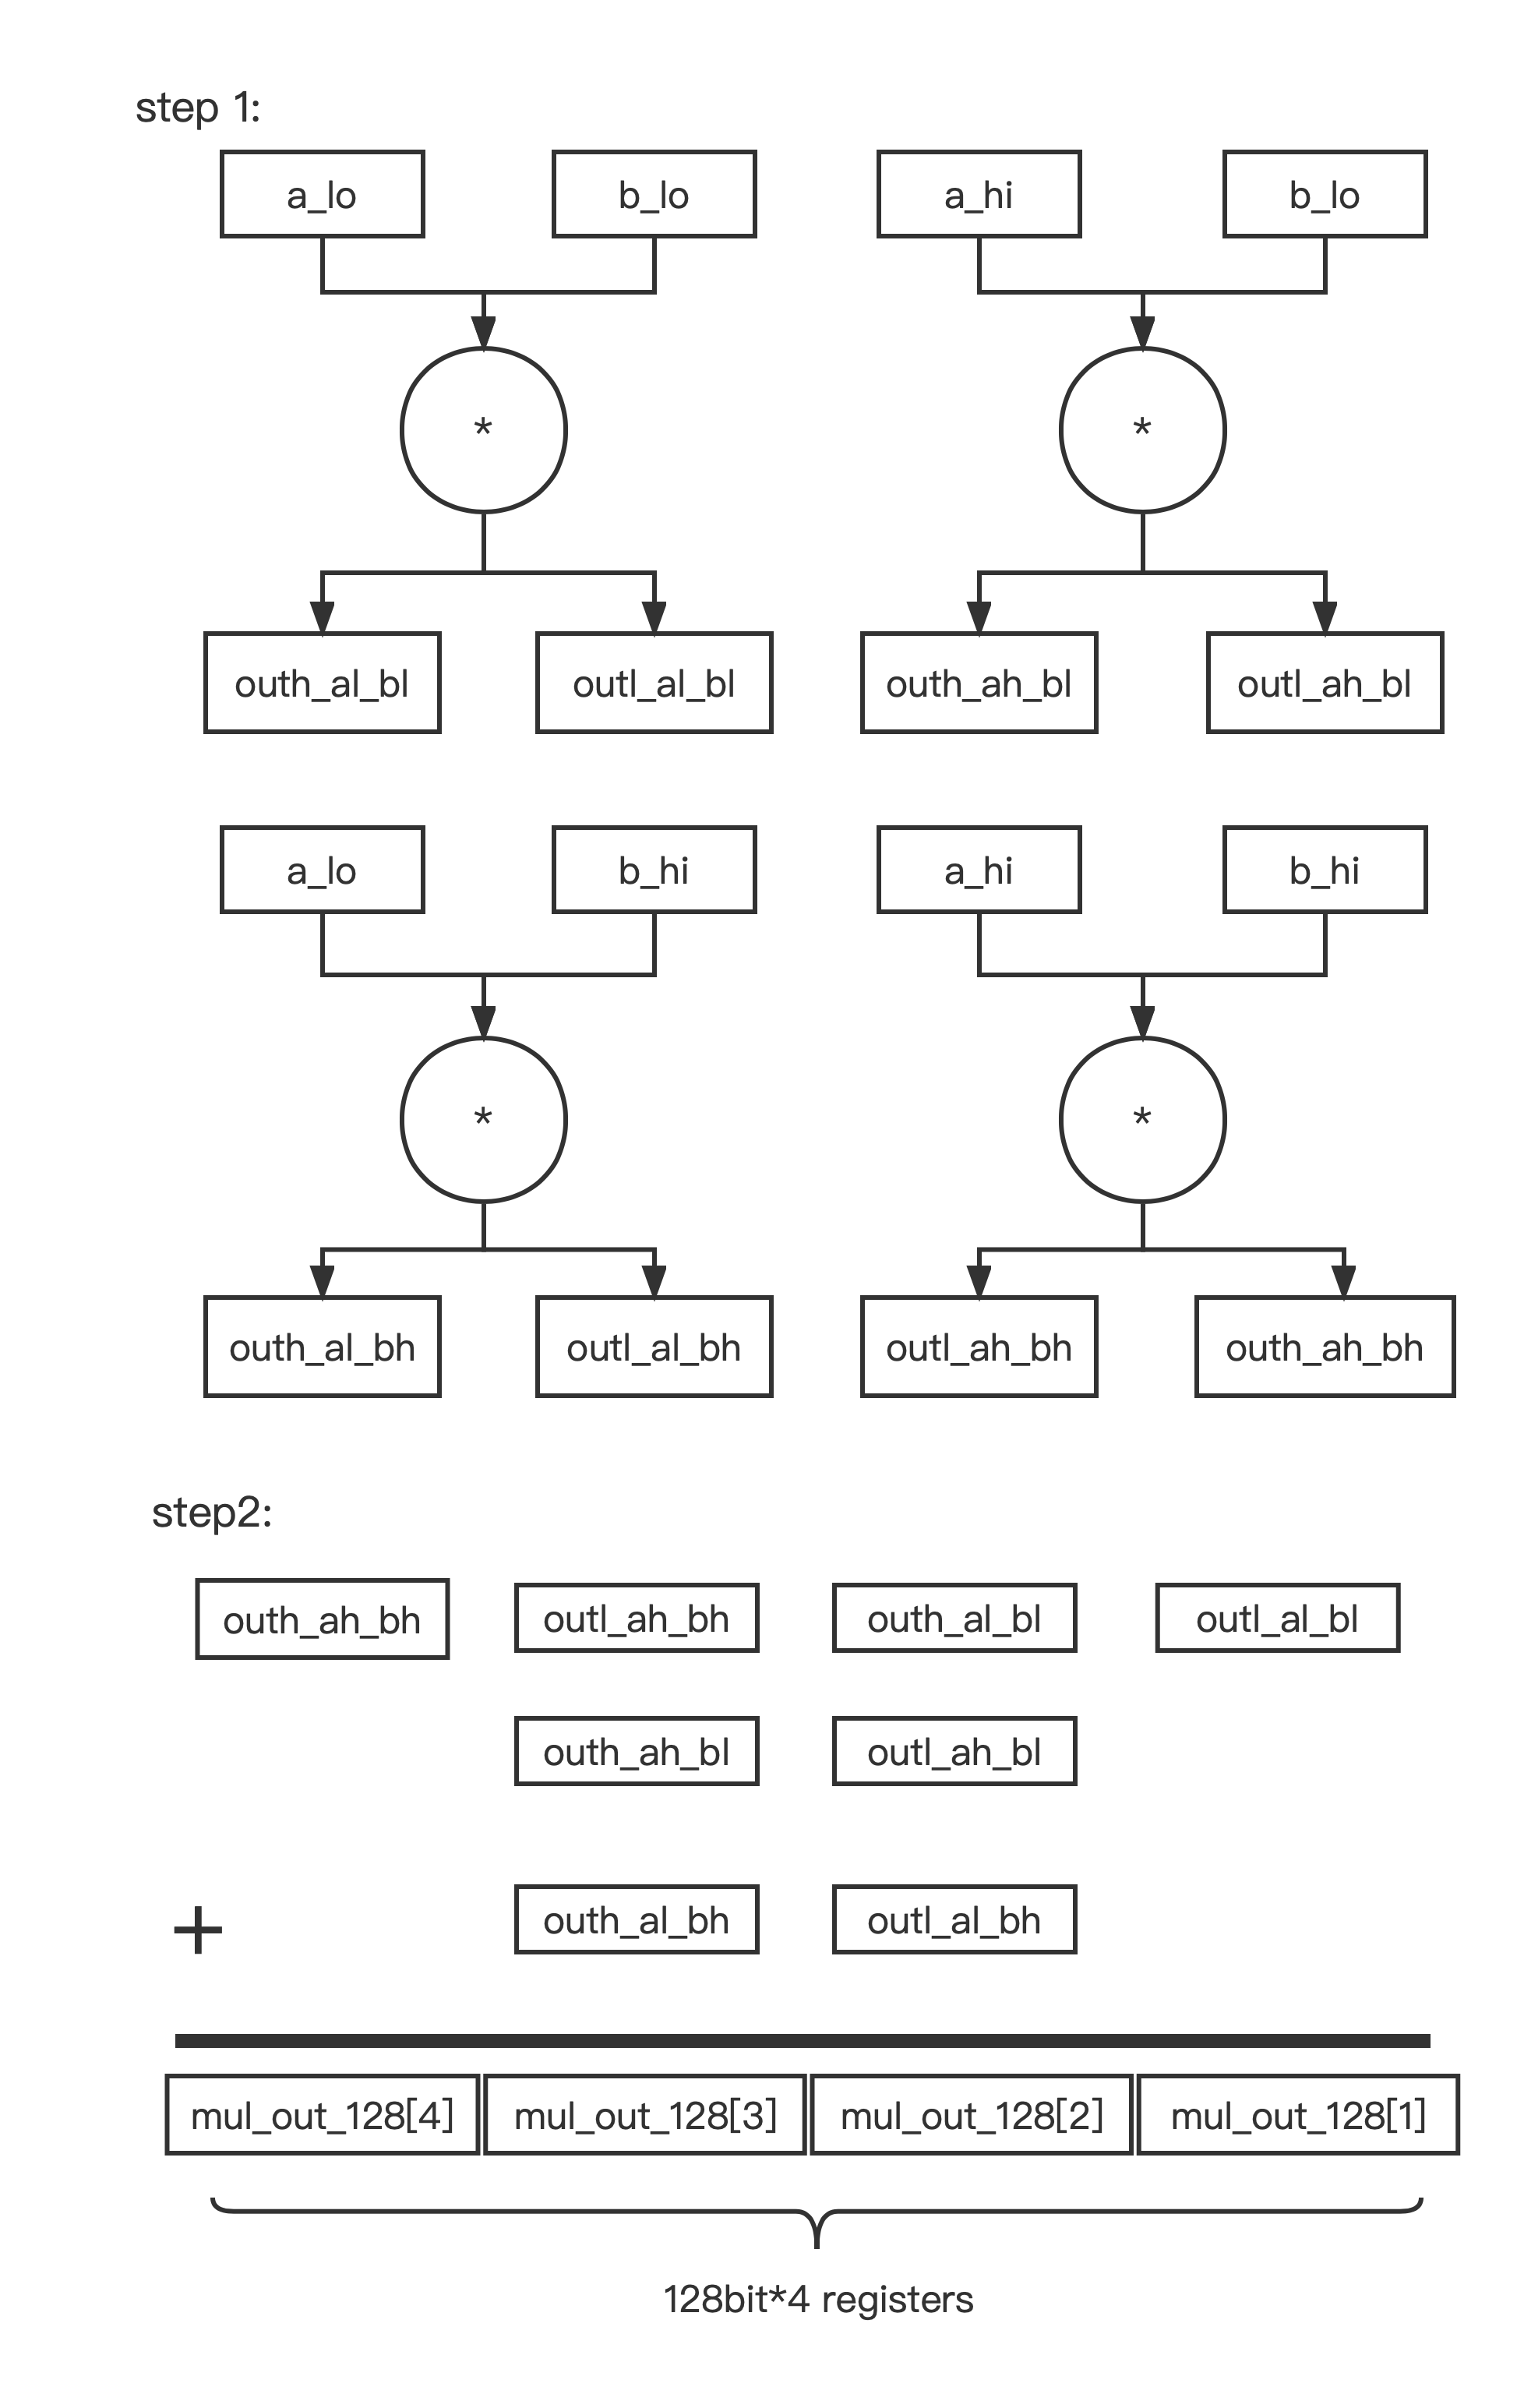
\includegraphics[width=0.8\textwidth]{u256-mul.png}
    \caption{uint256 multiplication algorithm}
    \label{fig:u256-mul}
\end{figure}

The instructions corresponding to the multiplication of uint256 are
\begin{lstlisting}[language={}]
split128 r_a, r_a_lo, r_a_hi
split128 r_b, r_b_lo, r_b_hi
[r_src1] = [r_a_lo]
[r_src2] = [r_b_lo]
range_check(r_src1, MAX_uint128)
range_check(r_src2, MAX_uint128)
MUL r_dst_al_bl, r_src1, r_src2

[r_src1] = [r_a_hi]
[r_src2] = [r_b_lo]
range_check(r_src1, MAX_uint128)
range_check(r_src2, MAX_uint128)
MUL r_dst_ah_bl, r_src1, r_src2

[r_src1] = [r_a_lo]
[r_src2] = [r_b_hi]
range_check(r_src1, MAX_uint128)
range_check(r_src2, MAX_uint128)
MUL r_dst_al_bh, r_src1, r_src2

[r_src1] = [r_a_hi]
[r_src2] = [r_b_hi]
range_check(r_src1, MAX_uint128)
range_check(r_src2, MAX_uint128)
MUL r_dst_ah_bh, r_src1, r_src2

split128 r_dst_al_bl, r_dst_al_bl_lo, r_dst_al_bl_hi
split128 r_dst_ah_bl, r_dst_ah_bl_lo, r_dst_ah_bl_hi
split128 r_dst_al_bh, r_dst_al_bh_lo, r_dst_al_bh_hi
split128 r_dst_ah_bh, r_dst_ah_bh_lo, r_dst_ah_bh_hi

range_check(r_dst_al_bl_hi, MAX_uint128)
range_check(r_dst_ah_bl_lo, MAX_uint128)
[r_mul_out_128_1] = [r_dst_al_bl]

ADD r_mul_out_128_2, r_dst_al_bl_hi, r_dst_al_bl_hi
ADD r_mul_out_128_2, r_mul_out_128_2, r_dst_al_bh_lo

split128 r_mul_out_128_2, r_mul_out_128_2, r_mul_out_128_2_carry

ADD r_mul_out_128_3, r_mul_out_128_2_carry, r_dst_ah_bl_hi
ADD r_mul_out_128_3, r_mul_out_128_3, r_dst_al_bh_hi
ADD r_mul_out_128_3, r_mul_out_128_3, r_dst_ah_bh_lo

split128 r_mul_out_128_3, r_mul_out_128_3, r_mul_out_128_3_carry

ADD r_mul_out_128_4, r_mul_out_128_3_carry, r_dst_ah_bh_hi

%{
    r_mul_out_256_2 = r_mul_out_128_4 * 2^128 + r_mul_out_128_3
    r_mul_out_256_1 = r_mul_out_128_2 * 2^128 + r_mul_out_128_1
%}

return [r_mul_out_256_2], [r_mul_out_256_1]
\end{lstlisting}

The multiplication of uint256 is composed of several instructions. The instructions are constrained by corresponding constraints in Section \ref{subsec:field-arithmetic-constraints}. The independent constraint of multiplication is
\[ \texttt{[r\_mul\_out\_256\_2]} \cdot 2^{256} + \texttt{[r\_mul\_out\_256\_1]} - \texttt{a} \cdot \texttt{b} = 0. \]

\subsubsection{DIV}

\emph{Library function interface:} \verb|uint256_div(uint256 a, uint256 div)|

The instructions corresponding to the division of uint256 are
\begin{lstlisting}[language={}]
if div == 0:
    return 0, 0
%{
    quotient = a / div
    remainder = a % div
%}
[r_quotient] = quotient
(r_mul_out_256_2, r_mul_out_256_1) = uint256_mul(r_quotient, div)
[r_zero] = 0
EQ r_mul_out_256_2, r_zero

[r_rem] = remainder

(r_a_check, r_add_carry) = uint256_add(r_mul_out_256_1, r_rem)
EQ r_a_check, r_a
EQ r_add_carry, r_zero
return [r_quotient], [r_rem]
\end{lstlisting}

The division of uint256 is composed of several instructions. The instructions are constrained by corresponding constraints in Section \ref{subsec:field-arithmetic-constraints}. The independent constraint of division is
\[ \texttt{[r\_quotient]} \cdot \texttt{[r\_div]} + \texttt{[r\_rem]} - \texttt{[r\_a]} = 0. \]


    \section{ZK Without FFT} \label{sec:zk-without-fft}

\subsection{Lagrange Basis Polynomial}

According to Lagrange Interpolation Algorithm, given $n$ points $(x_0,y_0),\ldots,(x_{n-1},y_{n-1})$, there exists a unique polynomial with a degree less than $n$ passing through these $n$ interpolation points, which can be expressed as
\[ f(x) = \sum_{i=0}^{n-1} y_i \prod_{j \ne i} \frac{x-x_j}{x_i-x_j}. \]
Define Lagrange basis polynomial as
\[ L_i(x) = \prod_{j \ne i} \frac{x-x_j}{x_i-x_j}. \]
Then the above formula can be written as $f(x)=\sum_{i=0}^{n-1}y_iL_i(x)$. Let $v(x)=\prod_{i=0}^{n-1}(x-x_i)$, using the formal derivative of $v(x)$
\begin{align*}
    v'(x) &= \sum_{i=0}^{n-1}\prod_{j \ne i}(x_i-x_j), \\
    v'(x_i) &= \prod_{j \ne i}(x_i-x_j).
\end{align*}
we can simplify the Lagrange basis to
\[ L_i(x) = \prod_{j \ne i}\frac{x-x_j}{x_i-x_j} = \frac{v(x)}{v'(x)(x-x_i)}. \]
All polynomials with a degree less than $n$, form an $n$-dimensional vector space under polynomial addition. For a polynomial $f(x)$ of a degree less than $n$, \[ f(x) = \sum_{i=0}^{n-1} a_ix^i, \]
$1,x,\ldots,x^{n-1}$ is a basis of the vector space, and the coordinate $a_i$ is called the coefficient form of $f(x)$. On the other hand, \[ f(x) = \sum_{i=0}^{n-1}f(x_i)L_i(x), \]
Lagrange basis $L_i(x)$ is also a basis of the vector space, and the coordinate $f_i=f(x_i)$ is called the evaluation form of $f(x)$.
The FFT/IFFT algorithm enables the transformation of the coordinates between the two bases.

Next, we will study how to calculate {\Update the} exact division when the divisor is a polynomial of degree 1, i.e.\ given $f(a)=0$, calculate the value of $q(x)=f(x)/(x-a)$ at the interpolation point $x_i$.
When $x_m \ne a$, $q(x_m)=f_m/(x_m-a)$, when $x_m=a$, since the degree of $q(x)=f(x)/(x-x_m)$ is less than $n-1$, we only need $n-1$ values of interpolation points $x_0,\ldots,x_{m-1} ,x_{m+1},\ldots,x_{n-1}$ to uniquely determine $q(x)$.
\begin{align*}
    q(x) &= \frac{f(x)}{x-x_m} \\
    &= \sum_{i \ne m} \frac{f_i}{x_i-x_m} \prod_{{\Update \substack{j \ne i \\ j \ne m}}} \frac{x-x_j}{x_i-x_j} \\
    &= \sum_{i \ne m} \frac{f_i}{x-x_m} \prod_{j \ne i} \frac{x-x_j}{x_i-x_j} \\
    &= \sum_{i \ne m} \frac{f_i}{x-x_m} L_i(x) \\
    &= \sum_{i \ne m} \frac{f_i}{x-x_m} \frac{v(x)}{v'(x)(x-x_i)} \\
    &= \sum_{i \ne m} \frac{f_i}{v'(x_i)(x-x_i)} \cdot \prod_{i \ne m}(x-x_i).
\end{align*}
Then
\begin{align*}
    q_m = q(x_m) &= \sum_{i \ne m} \frac{f_i}{v'(x_i)(x_m-x_i)} \cdot \prod_{i \ne m}(x_m-x_i) \\
    &= \sum_{i \ne m} \frac{f_i}{x_m-x_i} \cdot \frac{v'(x_m)}{v'(x_i)}.
\end{align*}

For non-interpolation points $z \notin \{x_0, \ldots, x_{n-1}\}$, we can calculate its value {\Update easily}
\begin{align*}
    f(z) = \sum_{i=0}^{n-1}f_iL_i(z)
    &= \sum_{i=0}^{n-1}\frac{v(z)f_i}{v'(z)(z-x_i)} \\
    &= v(z) \sum_{i=0}^{n-1}\frac{f_i}{v'(x_i)(z-x_i)}.
\end{align*}
If the interpolation point takes the $n$-th root of unity: $x_i=\omega^i$, then we have
\[ v(x)=x^n-1, \qquad v'(x)=nx^{n-1}, \qquad v'(x_i)=n\omega^{-i}, \]
\[ q_m = \sum_{i \ne m} \frac{f_i}{\omega^m-\omega^i} \cdot \frac{n\omega^{-m}}{n\omega^{-i}}
= \sum_{i \ne m} \frac{\omega^{i-m} f_i}{\omega^m-\omega^i}, \]
\[ f(z) = (z^n-1) \sum_{i=0}^{n-1}\frac{f_i}{n\omega^{-i}(z-\omega^i)}
= \frac{z^n-1}{n}\sum_{i=0}^{n-1}\frac{f_i\omega^i}{z-\omega^i}. \]

\subsection{KZG Without FFT}

We can represent a polynomial using Lagrange basis in KZG commitment, thus avoiding the use of FFT. The specific changes can be found in Table \ref{table:kzg-without-fft}.

\begin{table}[!htp]
    \centering
    \begin{tabularx}{\textwidth}{|X|X|X|}
        \hline
        \multicolumn{1}{|c|}{\emph{Coefficient Form}} & \multicolumn{1}{c|}{\emph{Evalutaion Form}} \\ \hline
        \multicolumn{2}{|c|}{Notations} \\ \hline
        $\mathbb{F}$: finite field \newline
        $\lambda$: security parameters \newline
        $\mathbb{G}_1,\mathbb{G}_2,\mathbb{G}_T$: groups of prime order $p$ over ECC \newline
        $e \colon \mathbb{G}_1 \times \mathbb{G}_2 \to \mathbb{G}_T$: symmetric bilinear pairing \newline
        $g,h$: generators of $\mathbb{G}_1,\mathbb{G}_2$ \newline
        $t$: max degree \newline
        $\omega$: primitive $n$-th root of unity in $\mathbb{F}$ \newline
        &
        $\mathbb{F}$: finite field \newline
        $\lambda$: security parameters \newline
        $\mathbb{G}_1,\mathbb{G}_2,\mathbb{G}_T$: groups of prime order $p$ over ECC \newline
        $e \colon \mathbb{G}_1 \times \mathbb{G}_2 \to \mathbb{G}_T$: symmetric bilinear pairing \newline
        $g,h$: generators of $\mathbb{G}_1,\mathbb{G}_2$ \newline
        $t$: max degree \newline
        $\omega$: primitive $n$-th root of unity in $\mathbb{F}$ \newline
        $L_i$: Lagrange basis, such that $L_j(\omega^i)=\begin{cases}
            1 & i=j \\
            0 & i \ne j \\
        \end{cases}$ \\ \hline
        \multicolumn{2}{|c|}{Input} \\ \hline
        $\left\{ (\omega^0, \phi(\omega^0)), (\omega^1, \phi(\omega^1)), \ldots,(\omega^{n-1}, \phi(\omega^{n-1})) \right\}$
        & $\left\{ (\omega^0, \phi(\omega^0)), (\omega^1, \phi(\omega^1)), \ldots,(\omega^{n-1}, \phi(\omega^{n-1})) \right\}$ \\ \hline
        \multicolumn{2}{|c|}{Setup} \\ \hline
        SK: $\alpha \in \mathbb{F}_p$, generated by trusted authority \newline
        PK: $\left(g,\alpha g, \ldots, \alpha^t g\right)\in \mathbb{G}_1^{t+1},\ \left(h, \alpha h\right) \in \mathbb{G}_2^2$
        &
        SK: $\alpha \in \mathbb{F}_p$, generated by trusted authority \newline
        PK: $\left(g,\alpha g, \ldots, \alpha^t g\right)\in \mathbb{G}_1^{t+1},\ \left(h, \alpha h\right) \in \mathbb{G}_2^2$ \\ \hline
        \multicolumn{2}{|c|}{Commitment(PK, $\phi(x)$)} \\
        \hline
        Polynomial: $\displaystyle \phi(x)=\sum_{j=0}^{\deg\phi}\phi_jx^j$ (IFFT) \newline
        Commitment: $\displaystyle C=\sum_{j=0}^{\deg\phi}\phi_j(\alpha^jg)$
        &
        Polynomial: $\displaystyle \phi(x)=\sum_{j=0}^{n-1}\phi(\omega^j)L_j(x)$ \newline
        Commitment: $\displaystyle C=\sum_{j=0}^{n-1}\phi(\omega^j)L_j(\alpha)g$ \\ \hline
        \multicolumn{2}{|c|}{
            CreateWitness(PK, $\phi(z)$, $z$) \quad
            (Query point $z$ out of domain, used in IOPP)
        } \\ \hline
        Compute quotient polynomial: $\displaystyle \psi(x)=\frac{\phi(x)-\phi(z)}{x-z}$ \newline
        Commitment: $\displaystyle w_z=\sum_{j=0}^{\deg\psi}\psi_j(\alpha^jg)$
        &
        Evaluate out of domain: $\displaystyle \phi(z)=\frac{z^n-1}{n}\sum_{i=0}^{n-1}\frac{\psi(\omega^i)\omega^i}{z-\omega^i}$ \newline
        Compute quotient polynomial: $\displaystyle \psi(\omega^j)=\frac{\phi(\omega^j)-\phi(z)}{\omega^j-z}$ \newline
        Commitment: $\displaystyle w_z=\sum_{j=0}^{n-1}\psi(\omega^j)L_j(\alpha)g$ \\ \hline
        \multicolumn{2}{|c|}{
            CreateWitness(PK, $\phi(z)$, $z$) \quad
            (Query point $z$ in of domain, used in Verkle Tree)
        } \\ \hline
        Evaluate in the domain: $\displaystyle \phi(x)=\sum_{j=0}^{\deg\phi}\phi_jz^j$ \newline
        Compute quotient polynomial: $\displaystyle \psi(x)=\frac{\phi(x)-\phi(z)}{x-z}$ \newline
        Commitment: $\displaystyle w_z=\sum_{j=0}^{\deg\psi}\psi_j(\alpha^jg)$
        &
        Compute quotient polynomial \newline
        $\displaystyle \psi(\omega^j) = \begin{cases}
            \frac{\phi(\omega^j)-\phi(z)}{\omega^j-z} & \omega^j \ne z \\
            \sum_{\omega^i \ne z}\frac{(\phi(\omega^i)-\phi(z))\omega^i}{z(z-\omega^i)} & \omega^j=z
        \end{cases}$ \newline
        Commitment: $\displaystyle w_z=\sum_{j=0}^{n-1}\psi(\omega^j)L_j(\alpha)g$ \\ \hline
        \multicolumn{2}{|c|}{VerifyEval(PK, $C$, $w_i$, $z$, $\phi(z)$)} \\ \hline
        Verify: $e(w_z, (\alpha-z)h) = e(C-\phi(z)g, h)$
        & Verify: $e(w_z, (\alpha-z)h) = e(C-\phi(z)g, h)$ \\ \hline
    \end{tabularx}
    \caption{KZG Commitment without FFT}
    \label{table:kzg-without-fft}
\end{table}

\subsection{FRI Decomposition}

We can write a polynomial $f(x)$ as the sum of odd and even power terms: $f(x)=f_e(x^2)+xf_o(x^2)$.
Let $\tilde{f}(x)=f(-x)$, then
\[
    f_e(x^2) = \frac{f(x)+f(-x)}{2} = \frac{f(x)+\tilde{f}(x)}{2},
    \quad
    f_o(x^2) = \frac{f(x)-f(-x)}{2x} = \frac{f(x)-\tilde{f}(x)}{2x}.
\]

\begin{lemma} \label{lemma:fri-decomposition}
    Let $H$ be an even-order subgroup of $\mathbb{F}_p^*$, $a,b,c,d$ be polynomials on the Lagrange basis of $H$, and $r$ be a random number.
    Let $H'=\{h^2 : h \in H\}$,
    \begin{align*}
        a' &= a_e + ra_o, \\
        b' &= b_e + rb_o, \\
        c' &= c_e + rc_o, \\
        d' &= r^2d_e/x + rd_o,
    \end{align*}
    which are polynomials on the Lagrange basis of $H'$, then
    \[
        \left\{ \begin{aligned}
            & ab = c + d \\
            & a\tilde{b} = c - d
        \end{aligned} \right.
        \ \Longleftrightarrow \
        \left\{ \begin{aligned}
            & a'b' = c' + d' \\
            & a'\tilde{b}' = c' - d'
        \end{aligned} \right. .
    \]
\end{lemma}
The proof of Lemma \ref{lemma:fri-decomposition} can refer to \cite{website:hadamard-check-without-fft}.

We can build a recursive proof protocol without FFT using Lemma \ref{lemma:fri-decomposition}.
Set $\omega$ to be a primitive root of unity of order $2^m$, $H_0=\langle\omega\rangle$ be the subgroup generated by $\omega$.
In order to prove the polynomial equation $ab=h$, we construct the polynomial on the Lagrange basis of $H_0$: $a^{(0)}=a$, $b^{(0)}=b$.
The prover first calculates the polynomials $c^{(0)}$, $d^{(0)}$, which produces
\[
    \left\{ \begin{aligned}
        & a^{(0)}b^{(0)} = c^{(0)} + d^{(0)} \\
        & a^{(0)}\tilde{b}^{(0)} = c^{(0)} - d^{(0)}
    \end{aligned} \right.
\]
and sends the KZG commitment of $a_0,b_0,c_0,d_0$ to the verifier.

The recursive proof requires $m$ rounds in total. In the $k$-th round, the prover starts from the commitments of $a^{(k)}_e,a^{(k)}_o,b^{(k)}_e,b^{(k)}_o,c^{(k)}_e,c^{(k)}_o,d^{(k)}_e/x,d^{(k)}_o$ that correspond to four polynomials $a^{(k)},b^{(k)},c^{(k)},d^{(k)}$ on the Lagrange basis of $H_k=\langle\omega^{2^k}\rangle$ and sends them to the verifier. The verifier replies with a random number $r$ and computes the corresponding commitment of $a',b',c',d'$.
In the next round, replace $H_k$ with $H_{k+1}$ and replace $a,b,c,d$ with $a^{(k+1)}=a',b^{(k+1)}=b',c^{(k+1)}=c',d^{(k+1)}=d'$ until $a^{(m)},b^{(m)},c^{(m)},d^{(m)}$ are reduced to constants after $m$ rounds and $|H_m|=1$.

Finally, the verifier randomly picks a point $z$ and performs multiple consistency verifications. For each polynomial $a^{(k)},b^{(k)},c^{(k)}$, the verifier needs to verify
\[
    \left\{ \begin{aligned}
        & f(z) = f_e(z^2) + zf_o(z^2) \\
        & f(-z) = f_e(z^2) - zf_o(z^2)
    \end{aligned} \right. .
\]
For polynomial $d^{(k)}$, the verifier needs to verify
\[
    \left\{ \begin{aligned}
        & f(z) = z^2(f_e/x)(z^2) + zf_o(z^2) \\
        & f(-z) = z^2(f_ex)(z^2) - zf_o(z^2)
    \end{aligned} \right. ,
\]
where $f$ represents some $a,b,c,d$, and $z$ is a random point.

The verifier also needs to verify the boundary conditions
\[
    \left\{ \begin{aligned}
        & a^{(m)}(z)b^{(m)}(z) = c^{(m)}(z) + d^{(m)}(z) \\
        & a^{(m)}(z)\tilde{b}^{(m)}(z) = c^{(m)}(z) - d^{(m)}(z)
    \end{aligned} \right. .
\]


    \section{ZK Acceleration} \label{sec:zk-acceleration}

The Zero Knowledge calculation process primarily consists of MSM, FFT/IFFT and polynomial evaluation. Given a circuit scale of approximately $2^{25}$, the rough computational consumption ratios are as shown in Figure \ref{fig:time-usage-origin}, ratios will vary for each unique scenario and algorithm.
\begin{figure}[!ht]
    \centering
    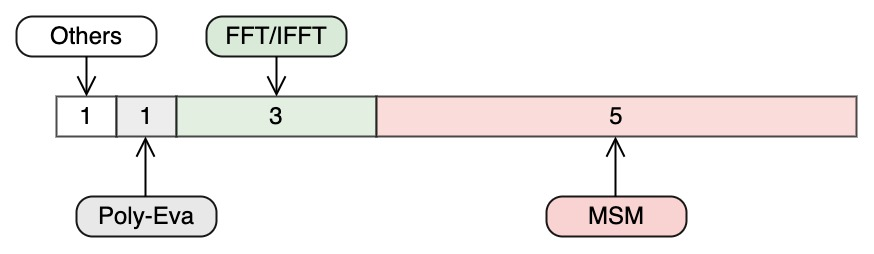
\includegraphics[width=0.8\textwidth]{zk-time-usage.jpg}
    \caption{Consumption ratios of each module of ZK calculation when $n \approx 2^{25}$}
    \label{fig:time-usage-origin}
\end{figure}

Do note that with an increased circuit size, consumption ratio of FFT/IFFT increases as well (because of the better parallelism implementation of MSM than FFT/IFFT), therefore, simply accelerating MSM and FFT/IFFT modules by GPU/FPGA to improve the speed of the prover is limited. We need a ZK algorithm without FFT, where the proportion of FFT/IFFT is so small that it can be ignored, so that the final consumption ratio of each module is close to Figure \ref{fig:time-usage-without-fft}.
\begin{figure}[!ht]
    \centering
    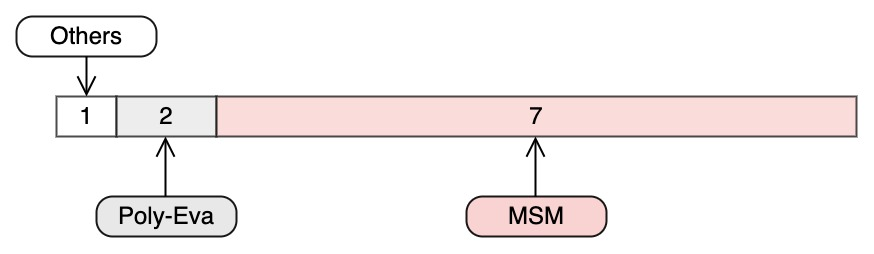
\includegraphics[width=0.8\textwidth]{zk-time-usage-without-fft.jpg}
    \caption{The consumption target ratio of each module of ZK calculation}
    \label{fig:time-usage-without-fft}
\end{figure}

We will introduce additional polynomials to eliminate FFT/IFFT calculations, thus generating additional MSM and polynomial evaluation operations, then using hardware-accelerated designs for MSM and polynomial evaluation operations.

\subsection{MSM of Variable Basis}

Given two vectors $(a_1,a_2,\ldots,a_n)$, $(G_1,G_2,\ldots,G_n)$, where $a_i$ is a field element, and $G_i$ is a point on the elliptic curve, MSM algorithm is to compute the following expressions: $\sum_{i=1}^n a_iG_i$.

\subsubsection{Windowing Method}

Assuming that the bit width of $a_i$ is $b$, we split it into multiple sub-modules with a bit width of $c$. Such sub-modules have a total of $k=\lceil b/c \rceil$, then
\[ a_iG_i = a_{i,0}G_i + 2^ca_{i,1}G_i + \cdots + 2^{(k-1)c}a_{i,k-1}G_i. \]
For all $i$ we have
\begin{align*}
    a_1G_1 &= a_{1,0}G_1 + 2^ca_{1,1}G_1 + \cdots + 2^{(k-1)c}a_{1,k-1}G_1, \\
    a_2G_2 &= a_{2,0}G_2 + 2^ca_{2,1}G_2 + \cdots + 2^{(k-1)c}a_{2,k-1}G_2, \\
    &\cdots \\
    a_nG_n &= a_{n,0}G_n + 2^ca_{n,1}G_n + \cdots + 2^{(k-1)c}a_{n,k-1}G_n.
\end{align*}
So
\[
    \sum_{i=1}^{n} a_iG_i =\sum_{i=1}^{n} \sum_{j=0}^{k-1} a_{i,j} 2^{jc} G_i
    =\sum_{j=0}^{m-1}\left(\sum_{i=1}^{n} a_{i,j} G_i\right) 2^{jc}.
\]
For $a_{i,j} \in [0,2^c)$, we can precompute
\[
    \begin{matrix}
        1G_1 & 2G_1 & \cdots & 2^{c-1}G_1 \\
        1G_2 & 2G_2 & \cdots & 2^{c-1}G_2 \\
        \vdots & \vdots & \ddots & \vdots \\
        1G_n & 2G_n & \cdots & 2^{c-1}G_n
    \end{matrix}
\]

\subsubsection{Endomorphism}

For a cyclic group $\mathbb{G}$ over an elliptic curve $y^2 = x^3 + ax + b$ on a finite field $\mathbb{F}_p$, if one can find such a group endomorphism $\varphi$:
there exists $\alpha, \beta \in \mathbb{F}_p$ such that $\varphi(x, y) = (\alpha x, \beta y)$ holds for all points on $\mathbb{G}$. It is easy to prove that such an automorphism is a multiplicative map, i.e.\ we can find a $\lambda$ such that $\varphi(P) = \lambda P$ holds for all points $P$ on $\mathbb{G}$. This means that when we know the coordinates of a point, we only need to multiply the $x$-coordinate and $y$-coordinate by a number in $\mathbb{F}_p$ to become the coordinates of another point, which can be used for further optimization of the algorithm. If the parameters of the elliptic curve are special, for example, BLS curves can be written as $y^2 = x^3 + b$, and $p \equiv 1 \pmod 3$, taking an element $\alpha$ of order 3 in $\mathbb{F}_p^*$, there exits a corresponding $\lambda$ such that $\lambda (x, y) = (\alpha x, y)$, then the multiplication operation can be optimized as
\begin{align*}
    mP &= (m_1 + m_2\lambda)P \\
    &= m_1P + m_2(\lambda P) \\
    &= m_1P + m_2\varphi(P).
\end{align*}

From \cite{scq03} we can find small $m_1$ and $m_2$ to make the above equation hold, i.e.\ $|m_1|, |m_2| < \sqrt{3 \cdot |\mathbb{G}|}$, which can reduce a multiplication operation of $b$ bits into two multiplication operations of $b/2$ bits. Applied to the windowing method, the number of group operations is reduced to \[ \frac{b}{c}(n+2^c-2) + b-c+\frac{b}{c}-1 \approx \frac{b}{c}(n+2^c). \]
When $n = 10^5$, it can save about 5.5\% of group operations.

\subsection{FPGA Acceleration}

The main flow of MSM calculation in FPGA is shown in Figure \ref{fig:fpga-acceleration}. When performing MSM of a large number of curve points, we mainly use Pippenger's algorithm \cite{pip76} to reduce the calculation of point doubling in MSM calculation process to improve calculation efficiency. Then perform a point addition on the buckets we get from the calculation.

\begin{figure}[!ht]
    \centering
    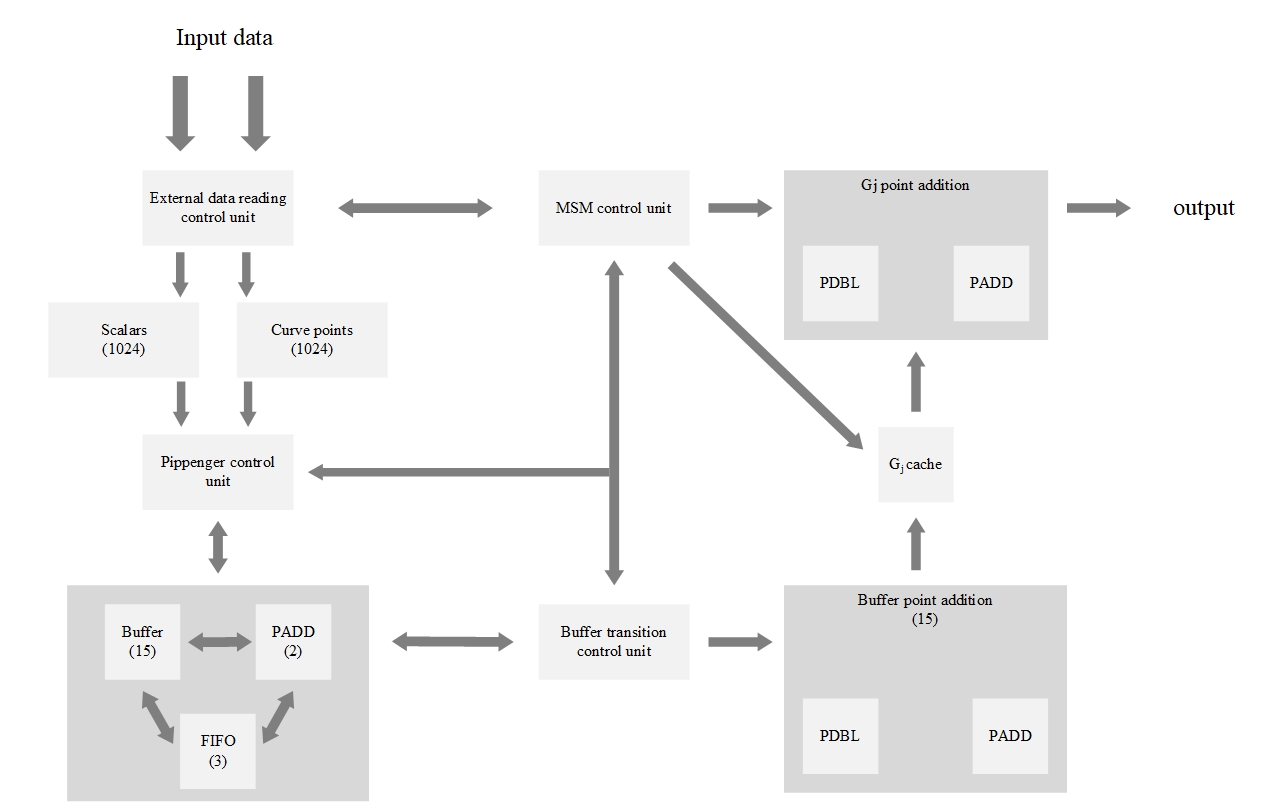
\includegraphics[width=0.8\textwidth]{fpga-acceleration.jpg}
    \caption{FPGA acceleration}
    \label{fig:fpga-acceleration}
\end{figure}

During the whole calculation process, we need a main control logic: MSM control logic, which completes the triggering of the external data reading logic, monitoring the status of the Pippenger control logic, Buffer transition and reading, point addition and point doubling control of the output results of Pippenger's algorithm. This is the brain of MSM.

The core process of the whole calculation is Pippenger's algorithm. In Pippenger's algorithm, firstly, read 1024 scalar values and 1024 curve points from the external memory through the external data reading control logic. Divide the scalar values into 4 bits, and then scan the curve points to complete PADD operation operation. It involves four modules in Pippenger's algorithm: the Pippenger control logic, Buffer, FIFO group and PADD operation. The Pippenger control logic mainly completes the division of sliding windows for scalar values, the cyclic extraction of curve point coordinates and the allocation, control of FIFO reading and writing, and the input and output of PADD. The Buffer buffers the output of PADD operation, while the FIFO group buffers the input of PADD operation.

Due to the limited on-chip memory of FPGA, Pippenger's algorithm can only perform MSM calculations of 1024 points each time. First up, extract the lowest 4 bits of the scalar values and perform point addition of 1024 points. After the addition operations, transfer the cache points in the Buffer, which requires the buffer transition control unit to complete. Secondly, after the point addition operations of 1024 scalars, the next Pippenger of 1024 points needs the Buffer transition control unit to load the Buffer point corresponding to the lowest 4 bits of last time. Then continue the operation, which will also be completed by the Buffer transition control unit.

After the point multiplication operations using Pippenger's algorithm, we need to perform point doubling and point addition operations on the result of the Buffer cache points we get from calculations. Finally, output the operation result of MSM.


    \section{Key Technologies} \label{sec:key-technologies}

This section introduces the key technical principles used in the design of OlaVM.

\subsection{Permutation Argument}

\emph{Step 1: Label and define permutation index polynomial $S$}

Permutation Argument explicitly specifies the exact location of the equal value, just as $V_3(1) = V_5(0)$ shown in Figure \ref{fig:permutation-index-polynomial}. Therefore, we need to define a new polynomial to represent the index correspondence between different polynomials.

\begin{figure}[!ht]
    \centering
    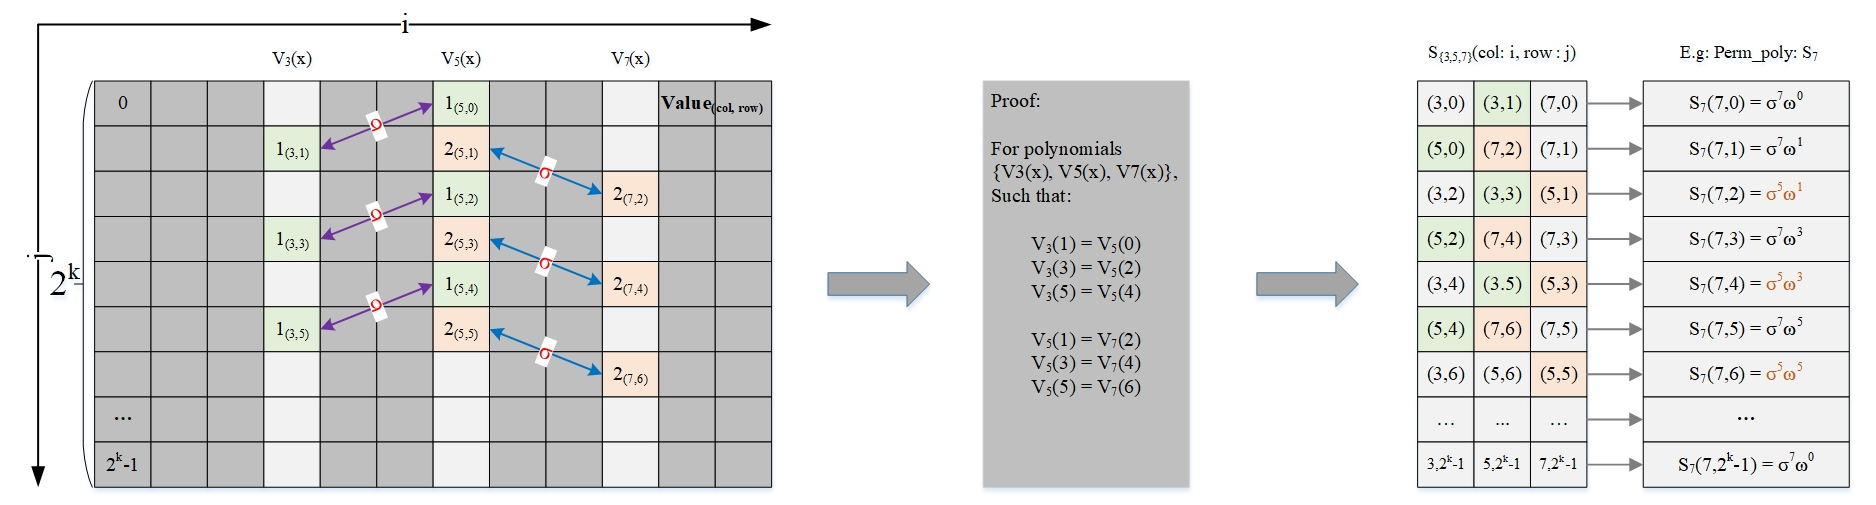
\includegraphics[width=\textwidth]{permutation-index-polynomial.jpg}
    \caption{Permutation index polynomial}
    \label{fig:permutation-index-polynomial}
\end{figure}

Since different polynomials correspond to different column indices, we can distinguish different evaluation domains by introducing column indices (distinguished through introducing a domain of size $n$ in Plonk, i.e.\ if there are $k$ polynomials, the domain size of \verb|perm_index_poly| is $kn$). The mapping can be expressed as
\[ S(\text{col:}i, \text{row:}j)=\sigma^{i'} \omega^{j'}. \]

Taking the polynomial $V_7(X)$ of column index = 7 as an example, the truth value of its corresponding permutation index polynomial $S_7(\text{col:}i, \text{row:}j)$ is shown in the right side of Figure \ref{fig:permutation-index-polynomial}.

\emph{Step 2: Generate the proof}

For the permutation index polynomial set $S = \{S_i\}$ generated based on step 1, we need to ensure the following equation holds:
\[
    \prod_{j=0}^{n-1} \frac{\left(V_3(\omega^j)+\beta \cdot \sigma^3 \cdot \omega^j+\gamma\right) \left(V_5(\omega^j)+\beta \cdot \sigma^5 \cdot \omega^j+\gamma\right) \left(V_7(\omega^j)+\beta \cdot \sigma^7 \cdot \omega^j+\gamma\right)} {\left(V_3(\omega^j)+\beta \cdot S(3, \omega^j)+\gamma\right) \left(V_5(\omega^j)+\beta \cdot S(5,\omega^{j})+\gamma\right) \left(V_7(\omega^j)+\beta \cdot S(7,\omega^{j})+\gamma\right)} = 1.
\]

\emph{Note:} If we reorder the indices of three polynomials (starting from 0 regardless of the original order, then the polynomial indices will be 0, 1 and 2 successively), the above equation can be simply expressed as
\[ \prod_{i=0}^{m-1} \prod_{j=0}^{n-1} \frac{V_i(\omega^j)+\beta \cdot \sigma^i \cdot \omega^j+\gamma}{V_i(\omega^j)+\beta \cdot S_i(\omega^j)+\gamma}=1. \]

where the permutation index polynomial is defined as
\[ S_{\text{col:}i}\left(\omega^{\text{row:}j}\right)=\sigma^{i'} \omega^{j'}. \]

The principle is shown in Figure \ref{fig:accumulator-polynomial}.

\begin{figure}[!ht]
    \centering
    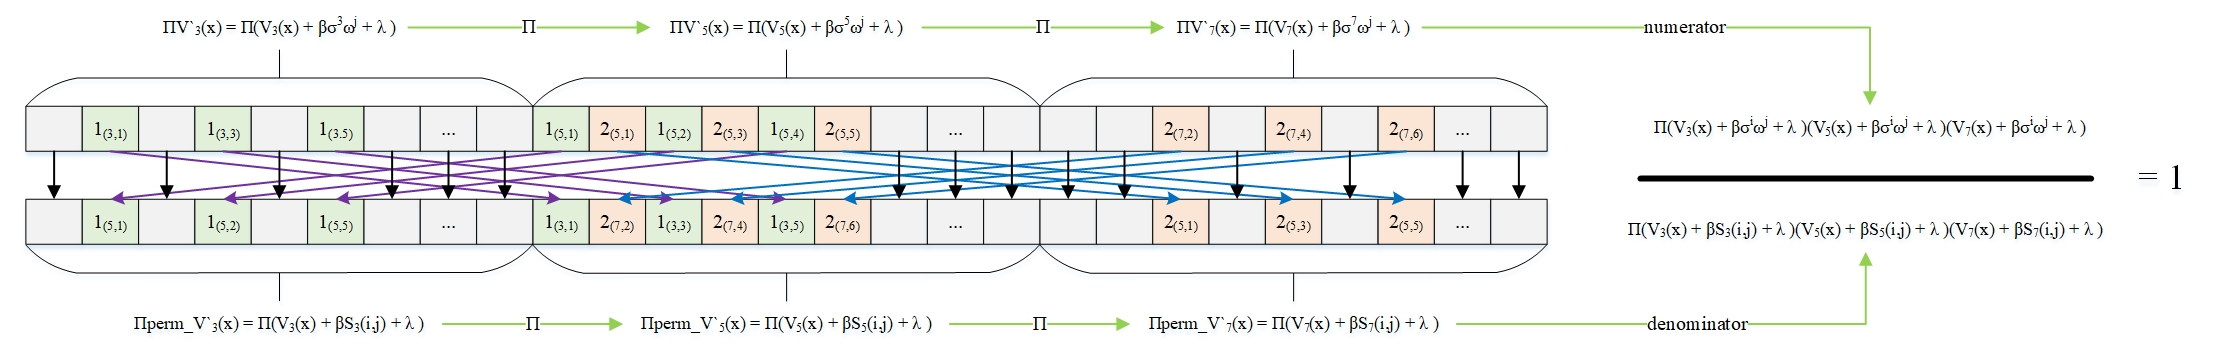
\includegraphics[width=\textwidth]{accumulator-polynomial.jpg}
    \caption{Accumulator polynomial}
    \label{fig:accumulator-polynomial}
\end{figure}

Due to the introduction of random numbers $\beta$ and $\gamma$, we can guarantee the two cells connected by purple lines and blue lines in Figure \ref{fig:accumulator-polynomial} to be equal with a probability close to 1 if and only if the copy constraints are satisfied according to Schwartz-Zippel Lemma. Finally, the multiplication result of the numerators is equal to that of denominators. Define the multiplicative polynomial $Z_P$ as follows:
\begin{align*}
    Z_P(W^0) &= 1, \\
    Z_P(W^{j+1}) &= \prod_{h=0}^j \prod_{i=0}^{m-1}\frac{V_i(\omega^h)+\beta \cdot \sigma^i \cdot \omega^h+\gamma}{V_i(\omega^h)+\beta \cdot S_i(\omega^h)+\gamma} \\
    &= Z_P(W^j)\prod_{i=0}^{m-1}\frac{V_i(\omega^{j})+\beta \cdot \sigma^{i} \cdot \omega^j+\gamma}{V_i(\omega^j)+\beta \cdot S_i(\omega^j)+\gamma}.
\end{align*}

It should satisfy the following constraints
\begin{align*}
    Z_P(\omega X) \prod_{i=0}^{m-1}\left(V_i(x)+\beta \cdot S_i(X)+\gamma\right) - Z_P(X) \prod_{i=0}^{m-1}\left(V_i(X)+\beta \cdot \sigma^{i} \cdot X+\gamma\right)=0, \\
    l_0 \cdot\left(1-Z_P(X)\right)=0.
\end{align*}

For further understanding of the principle, see Permutation Argument \cite{website:permutation-argument}.

\subsection{Lookup Argument}

Lookup Argument is used to prove that the elements of the two sets are of the same type, while the size can differ, therefore, for two sets $A$ and $S$, if we want to prove that they contain the same elements, first we need to remove duplicates and then we obtain two new sets $A'$ and $S'$. By performing LDT on them, we obtain two polynomials $A'(X)$ and $S'(X)$. According to the Schwartz-Zippel Lemma, we can know that the following constraints stand if and only if the set $A'$ contain the same elements as $S'$.
\begin{align*}
    Z(\omega X)(A'(X)+\beta)(S'(X)+\gamma) - Z(X)(A(X)+\beta)(S(X)+\gamma) = 0, \\
    (1-Z(X))l_0(X) = 0.
\end{align*}

For further understanding of the principle, refer to Lookup Argument \cite{website:lookup-argument} and Plookup \cite{cryptoeprint:2020/315}.

\subsection{Combined Selector}

This section mainly introduces how to improve the efficiency of ZK by combining selectors. First up, it introduces why selectors appear, and then how to combining multiple selectors.

\subsubsection{Custom Gate}

When designing ZKVM circuit, many binary selectors are introduced due to the vast amount of custom gates. Looking at the field division gate as an example, we plan to design a gate to verify the equation $q = x/y$ between three field elements $q,x,y$. For convenience, we will not implement field division operation at circuit level, but by checking the equations
\begin{align*}
& x \cdot y^{-1} = q, \\
& y^{-1} \cdot y = 1, \quad (\text{ensure $y \ne 0$}).
\end{align*}
They are equivalent, so we have the following trace table:
\begin{table}[!ht]
\centering
\begin{tabular}{|c|c|c|c|c|c|c|c|c|c|}
\hline
clk & $s_*$ & $\cdots$ & $s_\text{div}$ & $\cdots$ & $w_0$ & $w_1$ & $w_2$ & $w_3$ & Notes \\
\hline
$\cdots$ & $\cdots$ & $\cdots$ & $\cdots$ & $\cdots$ & $\cdots$ & $\cdots$ & $\cdots$ & $\cdots$ & $\cdots$ \\
\hline
$k$ & 0 & 0 & 1 & 0 & $x$ & $y$ & $q$ & $y^{-1}$ & division \\
\hline
$\cdots$ & $\cdots$ & $\cdots$ & $\cdots$ & $\cdots$ & $\cdots$ & $\cdots$ & $\cdots$ & $\cdots$ & $\cdots$ \\
\hline
\end{tabular}
\caption{A simple example of execution trace}
\end{table}

For columns $w_0,w_1,w_2,w_3$, define polynomials $w_0(x),w_1(x),w_2(x),w_3(x)$, then on the row corresponding to the division operation, they should satisfy
\begin{align*}
w_0(x) \cdot w_3(x) - w_2(x) &= 0, \\
w_1(x) \cdot w_3(x) - 1 &= 0.
\end{align*}

In order to ensure the satisfaction of the above relationships on the corresponding row, it is necessary to enable the corresponding division to constrain the verification through a selector, for which we introduce a new column, like $s_\text{div}= \{0,0,\ldots,1,\ldots,0\}$. After converting to polynomial $s_\text{div}(x)$, the above equations become
\begin{align*}
s_\text{div}(x)\cdot(w_0(x) \cdot w_3(x) - w_2(x)) &= 0, \\
s_\text{div}(x)\cdot(w_1(x) \cdot w_3(x) - 1) &= 0.
\end{align*}

\subsubsection{Combined Selector}

According to the above example, we know that whenever we define a new custom gate, we need to introduce a selector column $s_*$ related to the gate, called $t_*(x)$, then we have the following constraints
\begin{align*}
s_\text{add}(x) \cdot t_\text{add}(x) &= 0, \\
s_\text{div}(x) \cdot t_\text{div}(x) &= 0, \\
s_\text{cube}(x) \cdot t_\text{cube}(x) &= 0, \\
s_\text{sqrt}(x) \cdot t_\text{sqrt}(x) &= 0.
\end{align*}

Since the prover needs to make commitments to all polynomials when generating proofs, the introduction of too many selector polynomials will increase the workload of both the prover and verifier. Therefore, we need to optimize the number of selectors, which requires to meet two conditions:
\begin{enumerate}
    \item Without losing the meaning of selector polynomials, i.e.\ only specific gates can be allowed;
    \item Fewer selector polynomials.
\end{enumerate}

Plonky2 \cite{website:plonky2} shows a Binary-Tree based Selector optimization method, which reduces the number of selector polynomials to $\log(k)$, where $k$ is the number of custom gates; in Halo2 \cite{website:halo2}, ZCash team shares a new optimization method that may achieve a smaller number of polynomials (which is related to the constraint polynomial $t_*(x)$ and the parameter \verb|max_degree| set to the constraint polynomial).

We've taken forth a simple scenario to ease the understanding (for detailed algorithm, please refer to Selector Combining \cite{website:selector-combining}).

\begin{table}[!ht]
\centering
\begin{tabular}{|c|c|c|c|c|c|c|c|c|c|}
  \hline
  clk & $s_\text{add}$ & $s_\text{div}$ & $s_\text{cube}$ & $s_\text{sqrt}$ & $w_0$ & $w_1$ & $w_2$ & $w_3$ & Notes \\
  \hline
  0 & 1 & 0 & 0 & 0 & $a_0$ & $b_0$ & $c_0$ & $d_0$ & addition \\
  1 & 0 & 1 & 0 & 0 & $a_1$ & $b_1$ & $c_1$ & $d_1$ & division \\
  2 & 0 & 0 & 1 & 0 & $a_2$ & $b_2$ & $c_2$ & $d_2$ & cube \\
  3 & 0 & 0 & 0 & 1 & $a_3$ & $b_3$ & $c_3$ & $d_3$ & sqrt \\
  \hline
\end{tabular}
\caption{Multi-operation example of execution trace}
\end{table}

As can be seen, we have set 4 selector columns for the four custom gates, which are not what we want, thus increasing the workload of the prover and verifier. Then we define a new column $q$, satisfying
\begin{align*}
q = \begin{cases}
   k & \text{if the selector labelled } k \text{ is } 1 \\
   0 & \text{if all the selectors are } 0
\end{cases}.
\end{align*}

If we define a set $\{s_\text{add},s_\text{div},s_\text{cube},s_\text{sqrt}\}$ for selectors $s_\text{add},s_\text{div},s_\text{cube},s_\text{sqrt}$ (we call this set disjoint, because the rows enabled are not intersecting), combining the definition of column $q$, we have
\begin{table}[!ht]
\centering
\begin{tabular}{|c|c|c|c|c|c|c|c|c|c|c|}
  \hline
  clk & $s_\text{add}$ & $s_\text{div}$ & $s_\text{cube}$ & $s_\text{sqrt}$ & $q$ & $w_0$ & $w_1$ & $w_2$ & $w_3$ & Notes \\
  \hline
  0 & 1 & 0 & 0 & 0 & 1 & $a_0$ & $b_0$ & $c_0$ & $d_0$ & addition \\
  1 & 0 & 1 & 0 & 0 & 2 & $a_1$ & $b_1$ & $c_1$ & $d_1$ & division \\
  2 & 0 & 0 & 1 & 0 & 3 & $a_2$ & $b_2$ & $c_2$ & $d_2$ & cube \\
  3 & 0 & 0 & 0 & 1 & 4 & $a_3$ & $b_3$ & $c_3$ & $d_3$ & sqrt \\
  \hline
\end{tabular}
\caption{Add combined column $q$}
\end{table}

Then we define a new selector polynomial form based on column $q$. The $k$-th selector polynomial is
\[ q(x)\prod_{\substack{h=1 \\ h \ne k}}^{\mathrm{len}(\text{selectors})}(h - q(x)). \]
For example, for constraint $s_\text{add} \cdot t_\text{add}(x) = 0$, we can rewrite it as
\[ q(x)\prod_{\substack{h=1 \\ h \ne 1}}^{\mathrm{len}(\text{selectors})}(h - q(x)) \cdot t_\text{add}(x) = 0. \]
The above equation can be expanded into
\[ q(x)\cdot (2- q(x))\cdot(3-q(x))\cdot (4-q(x))\cdot t_\text{add}(x) = 0. \]
Define
\[ \mathrm{combined}_q(x) = q(x)\cdot (2- q(x))\cdot(3-q(x))\cdot (4-q(x)), \]
then we can derive its truth table:
\begin{table}[!ht]
    \centering
    \begin{tabular}{|c|c|c|}
      \hline
      clk & $\mathrm{combined}_q(x)$ & $s_\text{add}(x)$ \\
      \hline
      0 & 1 & 1 \\
      1 & 0 & 0 \\
      2 & 0 & 0 \\
      3 & 0 & 0 \\
      \hline
    \end{tabular}
    \caption{Consistency between $q$ and $s_\text{add}$}
\end{table}

This achieves the same function as the original selector, therefore, for constraints
\begin{align*}
s_\text{add}(x) \cdot t_\text{add}(x) &= 0, \\
s_\text{div}(x) \cdot t_\text{add}(x) &= 0, \\
s_\text{cube}(x) \cdot t_\text{cube}(x) &= 0, \\
s_\text{sqrt}(x) \cdot t_\text{sqrt}(x) &= 0.
\end{align*}
we can rewrite them as
\begin{align*}
q(x)\prod_{\substack{h=1 \\ h \ne 1}}^{\mathrm{len}(\text{selectors})}(h - q(x)) \cdot t_\text{add}(x) &= 0, \\
q(x)\prod_{\substack{h=1 \\ h \ne 2}}^{\mathrm{len}(\text{selectors})}(h - q(x)) \cdot t_\text{add}(x) &= 0, \\
q(x)\prod_{\substack{h=1 \\ h \ne 3}}^{\mathrm{len}(\text{selectors})}(h - q(x)) \cdot t_\text{cube}(x) &= 0, \\
q(x)\prod_{\substack{h=1 \\ h \ne 4}}^{\mathrm{len}(\text{selectors})}(h - q(x)) \cdot t_\text{sqrt}(x) &= 0.
\end{align*}

For constraints of the types above, we only need to make commitments to the polynomial $q(x)$. But we should note that this method also increases the degree of constraints.

So far, we have achieved the two points mentioned above:
\begin{enumerate}
    \item Without losing the meanings of selector polynomials, i.e.\ only specific gates can be allowed;
    \item Fewer selector polynomials.
\end{enumerate}

Of course, due to the limitation of degree of constraints in the protocol, the selectors that can be combined are limited. The number of selectors combined at a time depends on the degree of the constraint polynomial $t_*(x)$ and the boundary value \verb|max_degree|. Therefore, we may need multiple combined columns, even so the number of which is much smaller than the original number.

\subsection{Sinsemilla Hash}

Sinsemilla Hash is a Lookup Argument-friendly hash algorithm based on the complexity of discrete logarithm problem and collision resistance (the length of input is fixed). Compared with other algebraic hash algorithms, such as Rescue and Poseiden, Sinsemilla Hash has certain advantages and disadvantages:
\begin{itemize}
    \item Advantage: Sinsemilla Hash executes 19 times faster than Rescue and Poseiden Hash when executed out of circuit;
    \item Disadvantage: When executing with circuits, Sinsemilla Hash is 4 times slower than Rescue and Poseiden Hash.
\end{itemize}
Considering the local execution of hash calculation when generating the execution trace, Sinsemilla Hash is a better option from the perspective of the overall performance (ranging from data preparation to proof generation). Next let's take a look at the algorithm details of Sinsemilla Hash.

\subsubsection{Setup}

\begin{enumerate}
    \item Select the split parameter $k$;
    \item Generate $2^k+1$ independent points $\{Q, P_0, P_1, \ldots, P_{2^k-1}\}$.
\end{enumerate}

\subsubsection{Hash(M)}

\begin{enumerate}
    \item Split $M$ into $n$ groups of $k$ bits, the $i$-th group is represented as $m_i$ in little endian;
    \item Set the initial value $\mathrm{Acc}_0 = Q$.
    \item For $i$ from 0 to $n-1$, execute loop calculation $\mathrm{Acc}_{i+1} = (\mathrm{Acc}_i + P_{m_{i+1}}) + \mathrm{Acc}_i$.
    \item Finally we get $\mathrm{Acc}_n$.
    \item $\mathrm{ShortHash}(M)$ returns to the $x$-coordinate of $\mathrm{Hash}(M)$.
\end{enumerate}

\subsubsection{Incomplete Addition}

In step 3 of $\mathrm{Hash}(M)$, we have performed operation $\mathrm{Acc}_{i+1} = (\mathrm{Acc}_i + P_{m_{i+1}}) + \mathrm{Acc}_i$, where the elliptic curve addition algorithm used here is Incomplete addition, i.e., it can only process elliptic curve addition in valid input scenarios (the inputs are different points on the elliptic curve). The other one is a complete addition. The specific differences of the two calculation forms are shown in Incomplete and complete addition -- The halo2 Book \cite{website:halo2}.
\begin{itemize}
    \item Input: $P=(x_P,y_P)$, $Q=(x_Q,y_Q)$,
    \item Output: $R=P+Q=(x_R,y_R)$.
\end{itemize}

According to the introduction in Section 4.1 of \cite{quteprints33233}, the Incomplete addition formula can be expressed as
\begin{align*}
    x_R &= \left(\frac{y_Q-y_P}{x_Q-x_P}\right)^2 - x_Q - x_P, \\
    y_R &= \frac{y_Q-y_P}{x_Q-x_P} \cdot (x_Q - x_R) - y_Q.
\end{align*}

According to the definition of Incomplete addition, we have $x_Q \ne x_P$, so the previous formula can be transformed into
\begin{align*}
    & x_R = \left(\frac{y_Q-y_P}{x_Q-x_P}\right)^2 - x_Q-x_P \\
    \implies & x_R + x_Q + x_P = \left(\frac{y_Q-y_P}{x_Q-x_P}\right)^2 \\
    \implies & (x_R + x_Q + x_P)(x_Q - x_P)^2 - (y_Q - y_P)^2 = 0, \\
    & y_R = \frac{y_Q-y_P}{x_Q-x_P} \cdot (x_Q - x_R) - y_Q \\
    \implies & (y_R + y_Q)(x_Q - x_P) - (y_Q - y_P)(x_Q - x_R) = 0.
\end{align*}

So, for Incomplete addition of elliptic curve points, we have the following constraints:
\begin{table}[!ht]
    \centering
    \begin{tabular}{|c|c|}
        \hline
        \emph{Degree} & \emph{Constraint} \\
        \hline
        4 & $q_\text{incomplete-add} \cdot ((x_R + x_Q + x_P)(x_Q - x_P)^2 - (y_Q - y_P)^2) = 0$ \\
        3 & $q_\text{incomplete-add} \cdot ((y_R + y_Q)(x_Q - x_P) - (y_Q - y_P)(x_Q - x_R)) = 0$ \\
        \hline
    \end{tabular}
    \caption{Constraints for incomplete addition}
\end{table}

Let $\lambda=(y_Q-y_P)/(x_Q-x_P)$, the above constraints can be changed to:
\begin{table}[!ht]
    \centering
    \begin{tabular}{|c|c|}
        \hline
        \emph{Degree} & \emph{Constraint} \\
        \hline
        3 & $q_\text{incomplete-add} \cdot(x_R + x_Q + x_P - \lambda^2) = 0$ \\
        3 & $q_\text{incomplete-add} \cdot(\lambda(x_Q - x_R) - (y_Q + y_R)) = 0$ \\
        3 & $q_\text{incomplete-add} \cdot(\lambda(x_Q - x_P) - (y_Q - y_P)) = 0$ \\
        \hline
    \end{tabular}
    \caption{Improved constraints for incomplete addition}
\end{table}

\subsubsection{Lookup for Sinsemilla}

According to the calculation process of Sinsemilla, we need to split the original information $M$ into $n$ sub-information $m_i$ with a bit width of $k$ (since Sinsemilla has fixed-length input requirements, it's necessary to pad $M$ to a fixed length). Let $P_{m_i} = (x_{P,i}, y_{P,i})$, since $m_i \in [0,2^k)$, $k$ will not be large in general, then we can precompute a table for query as Table \ref{table:lookup-table-for-sinsemilla-hash}.

\begin{table}[!ht]
    \centering
    \begin{tabular}{|c|c|c|}
        \hline
        $i$ & $x$-coordinate & $y$-coordinate \\
        \hline
        $0$ & $x_{P,0}$ & $y_{P,0}$ \\
        $1$ & $x_{P,1}$ & $y_{P,1}$ \\
        $\cdots$ & $\cdots$ & $\cdots$ \\
        $2^k-1$ & $x_{P,2^k-1}$ & $y_{P,2^k-1}$ \\
        \hline
    \end{tabular}
    \caption{Lookup table for Sinsemilla Hash}
    \label{table:lookup-table-for-sinsemilla-hash}
\end{table}


    \section{Summary}

We covered the complete design of OlaVM in previous sections, including VM design, ZKVM constraint design, constraint ideas, logic behind each module and much more. We believe that this content will give a fundamental understanding of ZKVM design process. Due to the limited space, we are working on a new, detailed, ``module by module'' paper, focused on the subsequent engineering implementation process, which includes the design on how to support further EVM instructions in OlaVM. Related ZKVM technologies are under constant development and we continuously keep up to date with recent research, such as new ZK-friendly Hash and more efficient Lookup Argument \cite{cryptoeprint:2022/621}, in order to include this in OlaVM design.

In addition to this, we want to show our gratitude for the hard work of all the prominent teams in the space of Zero Knowledge, of which, naming a few, PSE, Matter Labs, Polygon Hermez and StarkWare. We have learnt a lot through their contributions in open source documentation, code and online sharing amongst other, on how to design, improve ZK-efficiency and construct a ZKVM. We want to direct a special thanks towards Justin Drake\footnote{\url{https://twitter.com/drakefjustin}}, Barry Whitehat\footnote{\url{https://twitter.com/barrywhitehat}} and others, whom we've had educational and inspirational information exchanges with, enlightening us on certain aspects in ZKEVM design, providing us with a better understanding on how to proceed. On an ending note, there is still a lot to be done, research to be conducted, knowledge to be acquired and room for improvement to be identified.


    \printbibliography[heading=bibintoc, title=\ebibname]
\end{document}
